\chapter{Análisis espectral de señales finitas}
\label{chap: estudio espectral}


\section{Motivación para realizar un estudio espectral de los PDL}
No es difícil convencerse de que las condiciones de ortogonalidad
impuestas en la definición de la base discreta de Legendre
\marginnote{En esta motivación informal, por ``oscilación''
de una señal $x = (x_{m})_{m=0}^{n-1}$
entendemos
tres cambios consecutivos de signo en sus entradas.}
$\cali{L}^{n}$
forzan a las entradas de los polinomios discretos $\cali{L}^{n,k}$
a cambiar más frecuentemente de signo conforme aumenta
el grado $k$, luego, conforme $k$ tiende a $n-1$,
la cantidad de oscilaciones aumenta; revisemos, 
por ejemplo, el caso $n=4$.



\begin{minipage}{0.5\textwidth}
\begin{figure}[H]
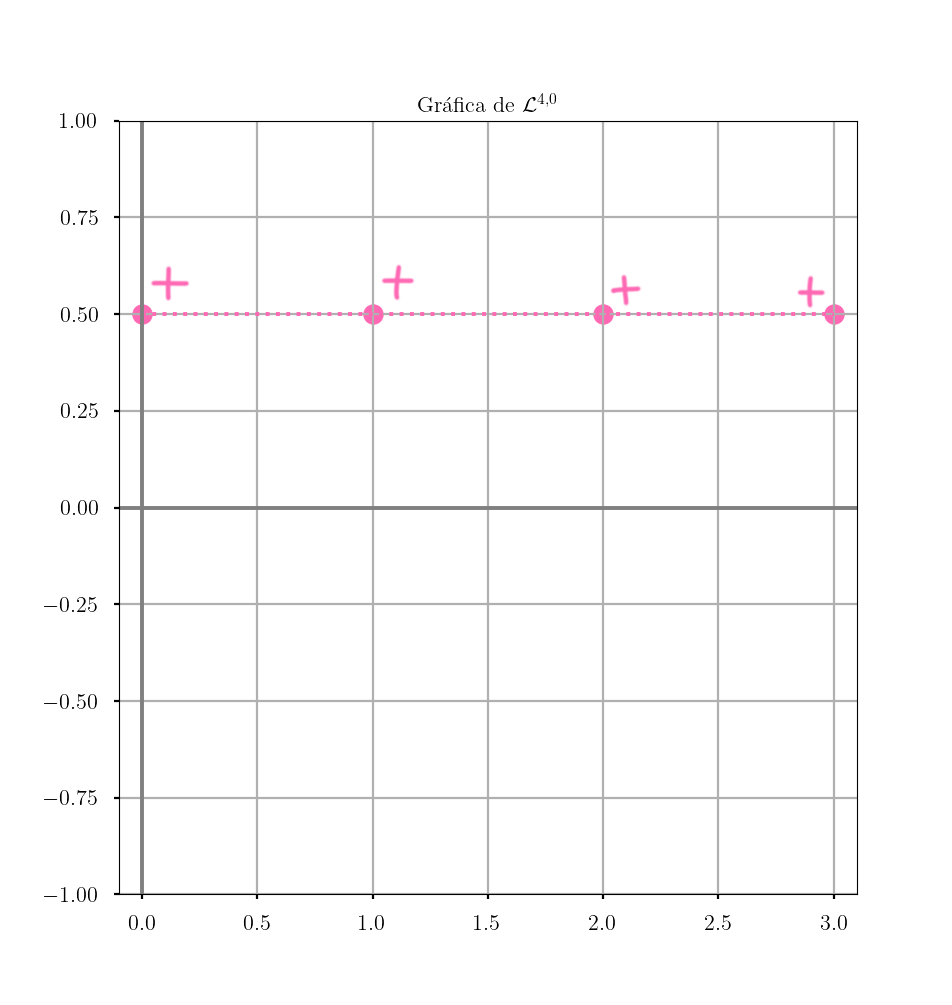
\includegraphics[scale=0.25]{oscil1}
\end{figure}
\end{minipage} \hfill
\begin{minipage}{0.45\textwidth}
1.- Por definición,
$\mathcal{L}^{4,0}$ se obtiene al normalizar 
al vector constante uno de $\IR^{4}$, o sea, 

\[
\cali{L}^{4,0} = \left(
\frac{1}{2}, \frac{1}{2}, \frac{1}{2}, \frac{1}{2}
\right).
\]
\end{minipage} 


\begin{minipage}{0.5\textwidth}
2.- La señal $\cali{L}^{4,1} \in \IR^{4}$ es un polinomio discreto de
dimensión 4 y grado 1 que se obtiene exigiendo las
siguientes condiciones

\[
\langle \cali{L}^{4,1} , \cali{L}^{4,0} \rangle=0
\hspace{0.2cm} \text{y} \hspace{0.2cm}
\langle \cali{L}^{4,1} , \cali{L}^{4,1} \rangle=1;
\]
esta primera condición se refleja en que 
las alturas de los puntos de la gráfica de 
$\cali{L}^{4,1}$ deben sumar cero;
esto implica un cambio de signo (y sólo uno,
pues el polinomio es lineal).

\end{minipage} \hfill
\begin{minipage}{0.45\textwidth}
\begin{figure}[H]
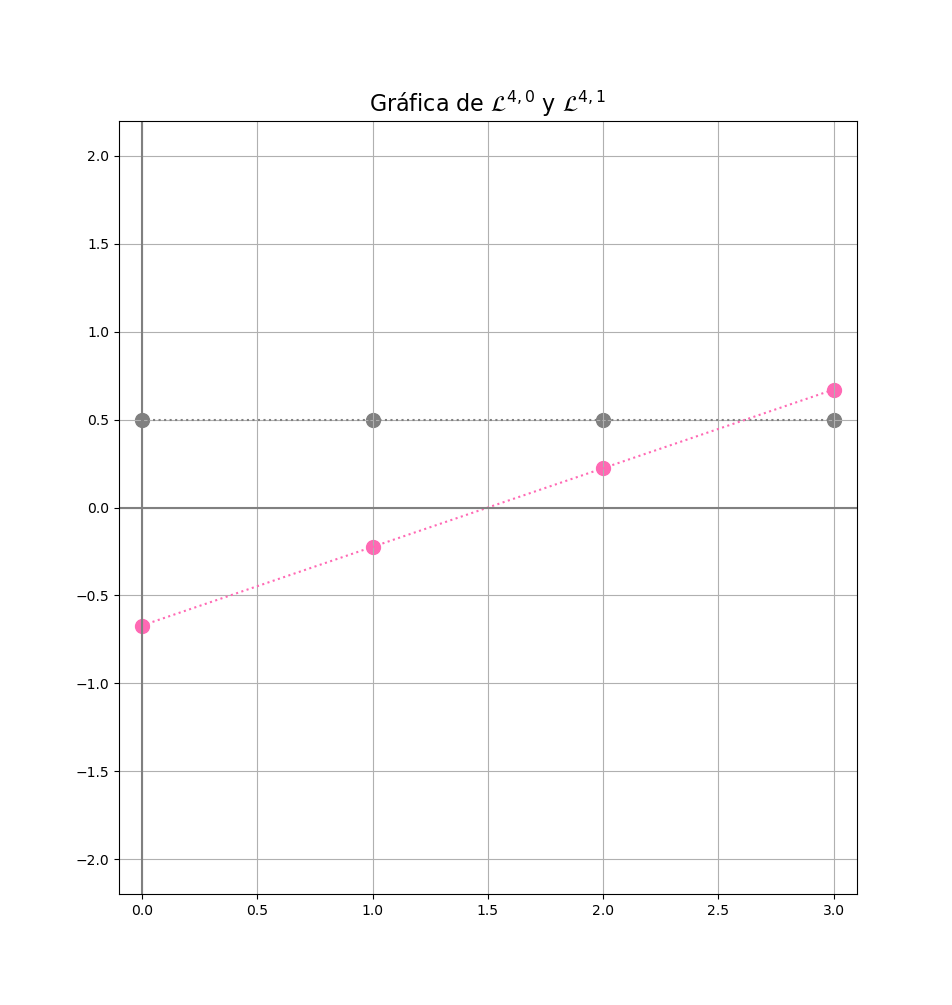
\includegraphics[scale=0.3]{oscil2}
\end{figure}
\end{minipage}

\noindent
3.- El vector
$\cali{L}^{4,2} \in \IR^{4}$,
que es un polinomio discreto
de grado $2$, satisface las siguientes
tres condiciones:

\[
\langle \cali{L}^{4,2} , \cali{L}^{4,0} \rangle=0,
\hspace{0.2cm}
\langle \cali{L}^{4,2} , \cali{L}^{4,1} \rangle=0,
\hspace{0.2cm} \text{y} \hspace{0.2cm}
\langle \cali{L}^{4,2} , \cali{L}^{4,2} \rangle=1.
\]
La segunda condición no da información sobre más
requerimientos que deba cumplir
$\cali{L}^{4,2}$, pues,
como $\cali{L}^{4,1} \in S_{n,-}$
y $\cali{L}^{4,2} \in S_{n,+}$
(c.f. teorema 
\ref{prop: simetrias en dimensiones pares}),
ya del lema
\ref{lema: ortogonalidad entre sim y antisim}
se deducía la ortogonalidad de estas señales; 
observe sin embargo que, si las entradas de 
$\cali{L}^{4,2}$ fuesen todas positivas o todas negativas,
entonces no se tendría la ortogonalidad
con la señal constante $\cali{L}^{4,0}$.


\begin{figure}[H]
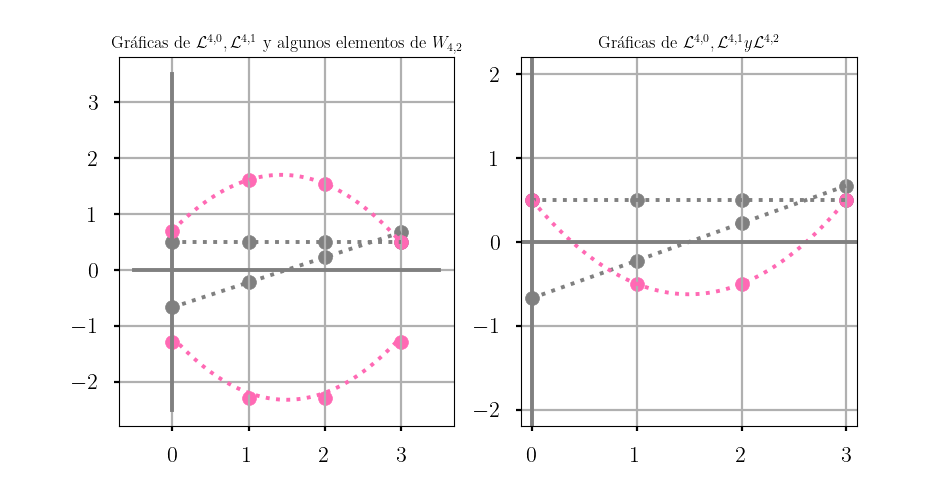
\includegraphics[scale=0.6]{oscil3}
\end{figure}

4.- Por último, $\cali{L}^{4,3} \in \IR^{4}$ satisface
las siguientes cuatro condiciones: 

\[
\langle \cali{L}^{4,3} , \cali{L}^{4,0} \rangle=0,
\hspace{0.2cm}
\langle \cali{L}^{4,3} , \cali{L}^{4,1} \rangle=0,
\langle \cali{L}^{4,3} , \cali{L}^{4,2} \rangle=0,
\hspace{0.2cm} \text{y} \hspace{0.2cm}
\langle \cali{L}^{4,3} , \cali{L}^{4,3} \rangle=1.
\]

Según los teoremas 
\ref{cor: propiedades importantes de espacios Wi}
y \ref{prop: simetrias en dimensiones pares},
$\cali{L}^{4,3}$ es la discretización de un polinomio
cúbico y además es una señal antisimétrica (en el sentido de la definición
\ref{def: espacios de seniales simetricas y antisimetricas}); dos gráficas de señales que cumplen esto se ilustran abajo:

\begin{figure}[H]
	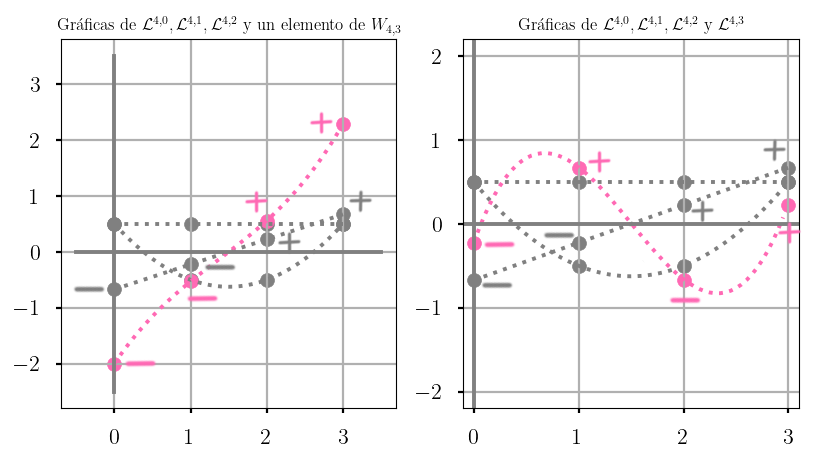
\includegraphics[scale=0.6]{oscil4}
	\sidecaption{Observe que la señal cúbica de la izquierda tiene
	un sólo cambio de signo, mientras que la de la derecha (que es 
	$\cali{L}^{4,3}$) tiene tres.}
\end{figure}

La señal cúbica de la izquierda, a pesar de 
ser ortogonal a $\mathcal{L}^{4,0}$ y a $\cali{L}^{4,2}$ por 
simetría (c.f. lema
\ref{lema: ortogonalidad entre sim y antisim}), 
definitivamente no puede ser ortogonal
a $\cali{L}^{4,1}$, pues las entradas de estos dos vectores de 
$\IR^{4}$ tienen el mismo signo. Sin embargo, la señal cúbica 
de la derecha (que de hecho es $\cali{L}^{4,3}$) sí cumple el ser
ortogonal a $\cali{L}^{4,1}$ pero, para lograr esto, sus
entradas deben cambiar de signo tres veces. \\


Después de graficar los PDL de otras dimensiones
puede apreciarse que esta tendencia a aumentar el número
de oscilaciones en las gráficas conforme el grado $k$
tiende a $n-1$ (su cota superior)
parece presentarse en todas las dimensiones.
Por ejemplo, abajo se muestran las gráficas de los 
PDL de dimensión $7$.

\begin{figure}[H]
	\centering
	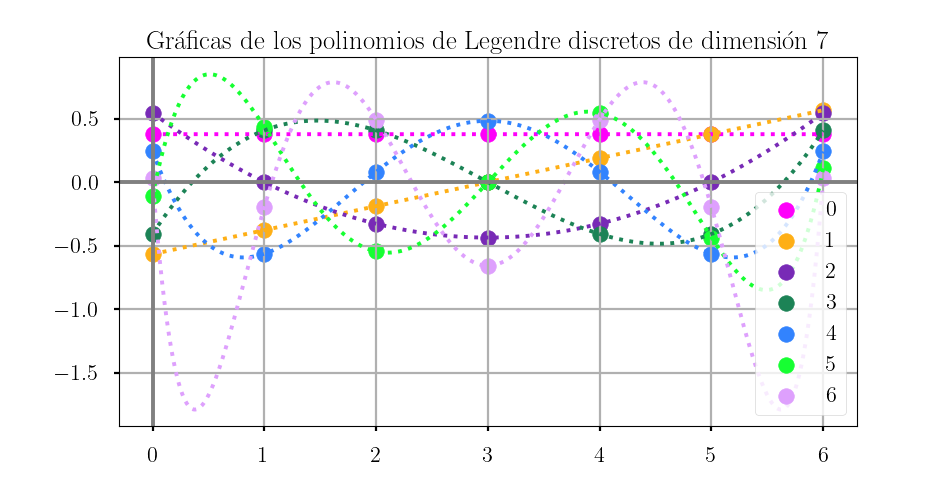
\includegraphics[scale = 0.55]{oscilaciones_dim7} 
\end{figure}	

\section{Hipótesis sobre las oscilaciones de los PDL}

Con el objetivo de analizar la forma
de oscilación de los PDL, nos proponemos
hacer un análisis espectral. Antes
de proceder sistemáticamente, hagamos un análisis empírico.
\begin{figure}[H]
	\sidecaption{
	Con ``sinusoide'' nos referimos a una función 
	continua cuya forma se ilustra en la figura. Este queda
	completamente determinado al fijar una
	\textbf{amplitud}, una \textbf{frecuencia} y un
	\textbf{desfase}, que nosotros preferimos normalizar
	para que sea un número entre $0$ y $1$.
	\label{fig: sinusoide}
	}
	\centering
	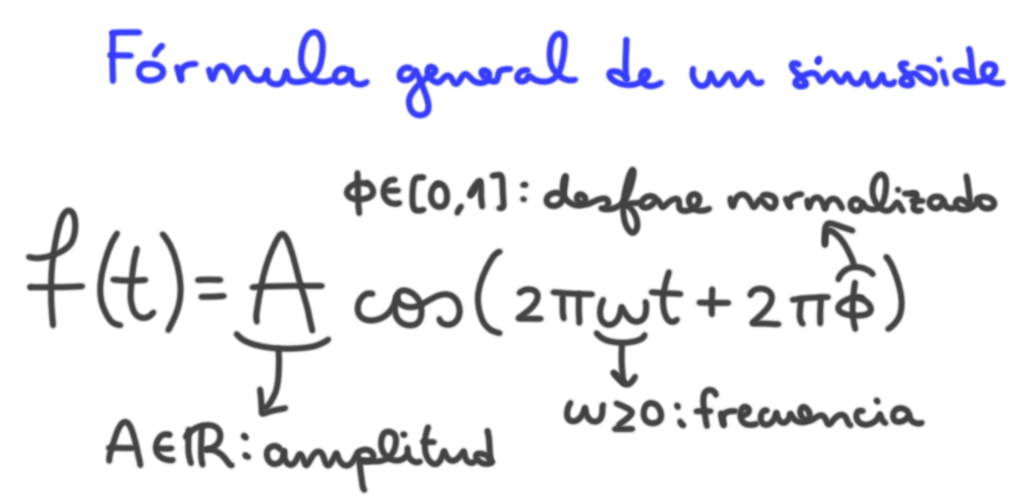
\includegraphics[scale = 0.8]{sinusoide} 
\end{figure}	

Pongamos una dimensión de $n = 60$. A continuación,
graficamos los PDL de dimensión $60$ para los primeros grados,
e intentamos aproximar tales gráficas con sinusoides continuos.


\begin{figure}[H]
	\sidecaption{
	Aproximando las gráficas
	de $\cali{L}^{60,0}$ y $\cali{L}^{60,1}$
	con sinusoides. 
	\label{fig: hip_0,1}
	}
	\centering
	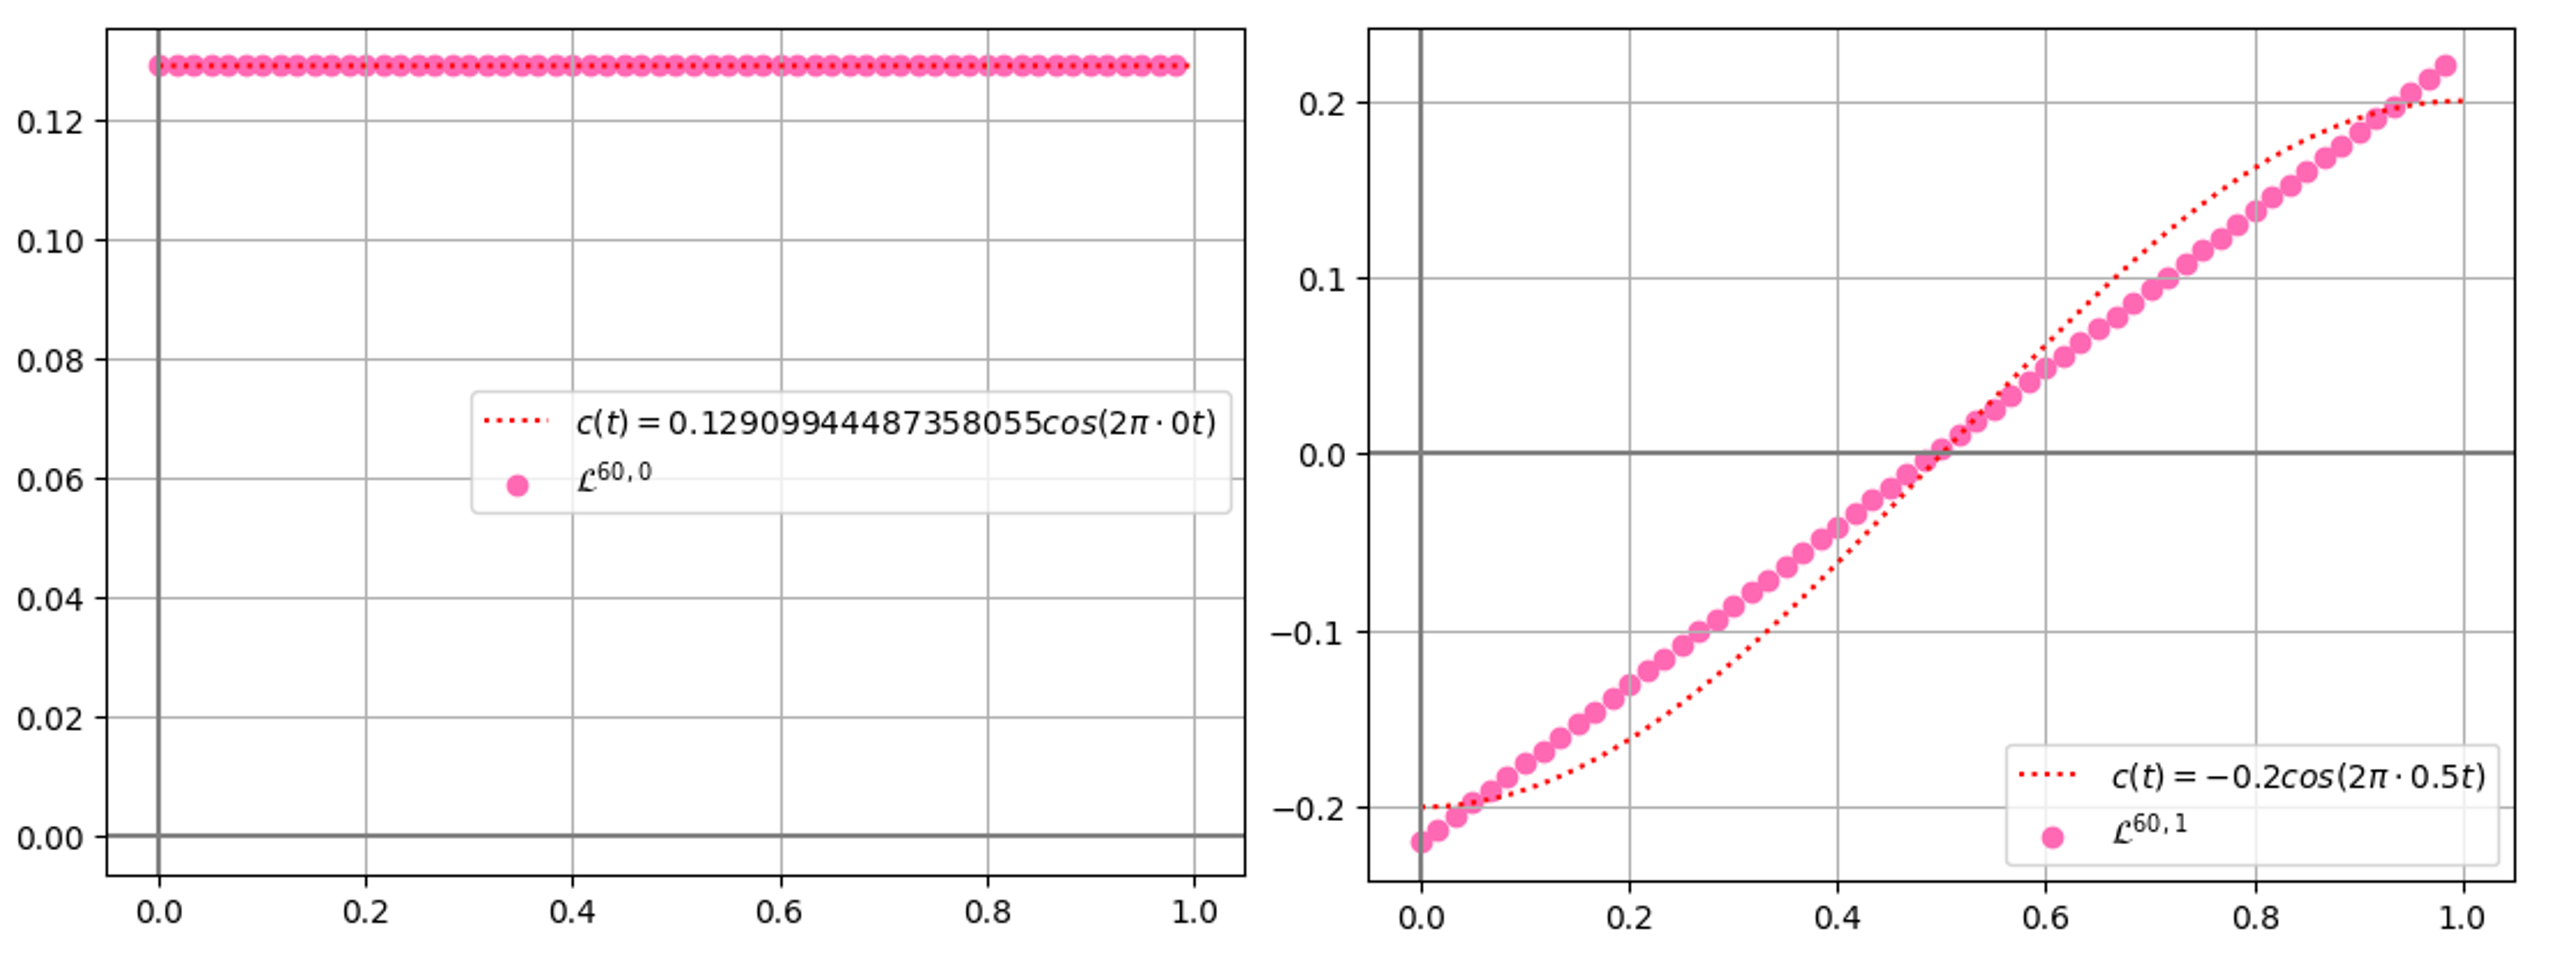
\includegraphics[scale = 0.6]{hip_0,1} 
\end{figure}	

\begin{figure}[H]
	\sidecaption{
	Aproximando las gráficas
	de $\cali{L}^{60,2}$ y $\cali{L}^{60,3}$
	con sinusoides. 
	\label{fig: hip_2,3}
	}
	\centering
	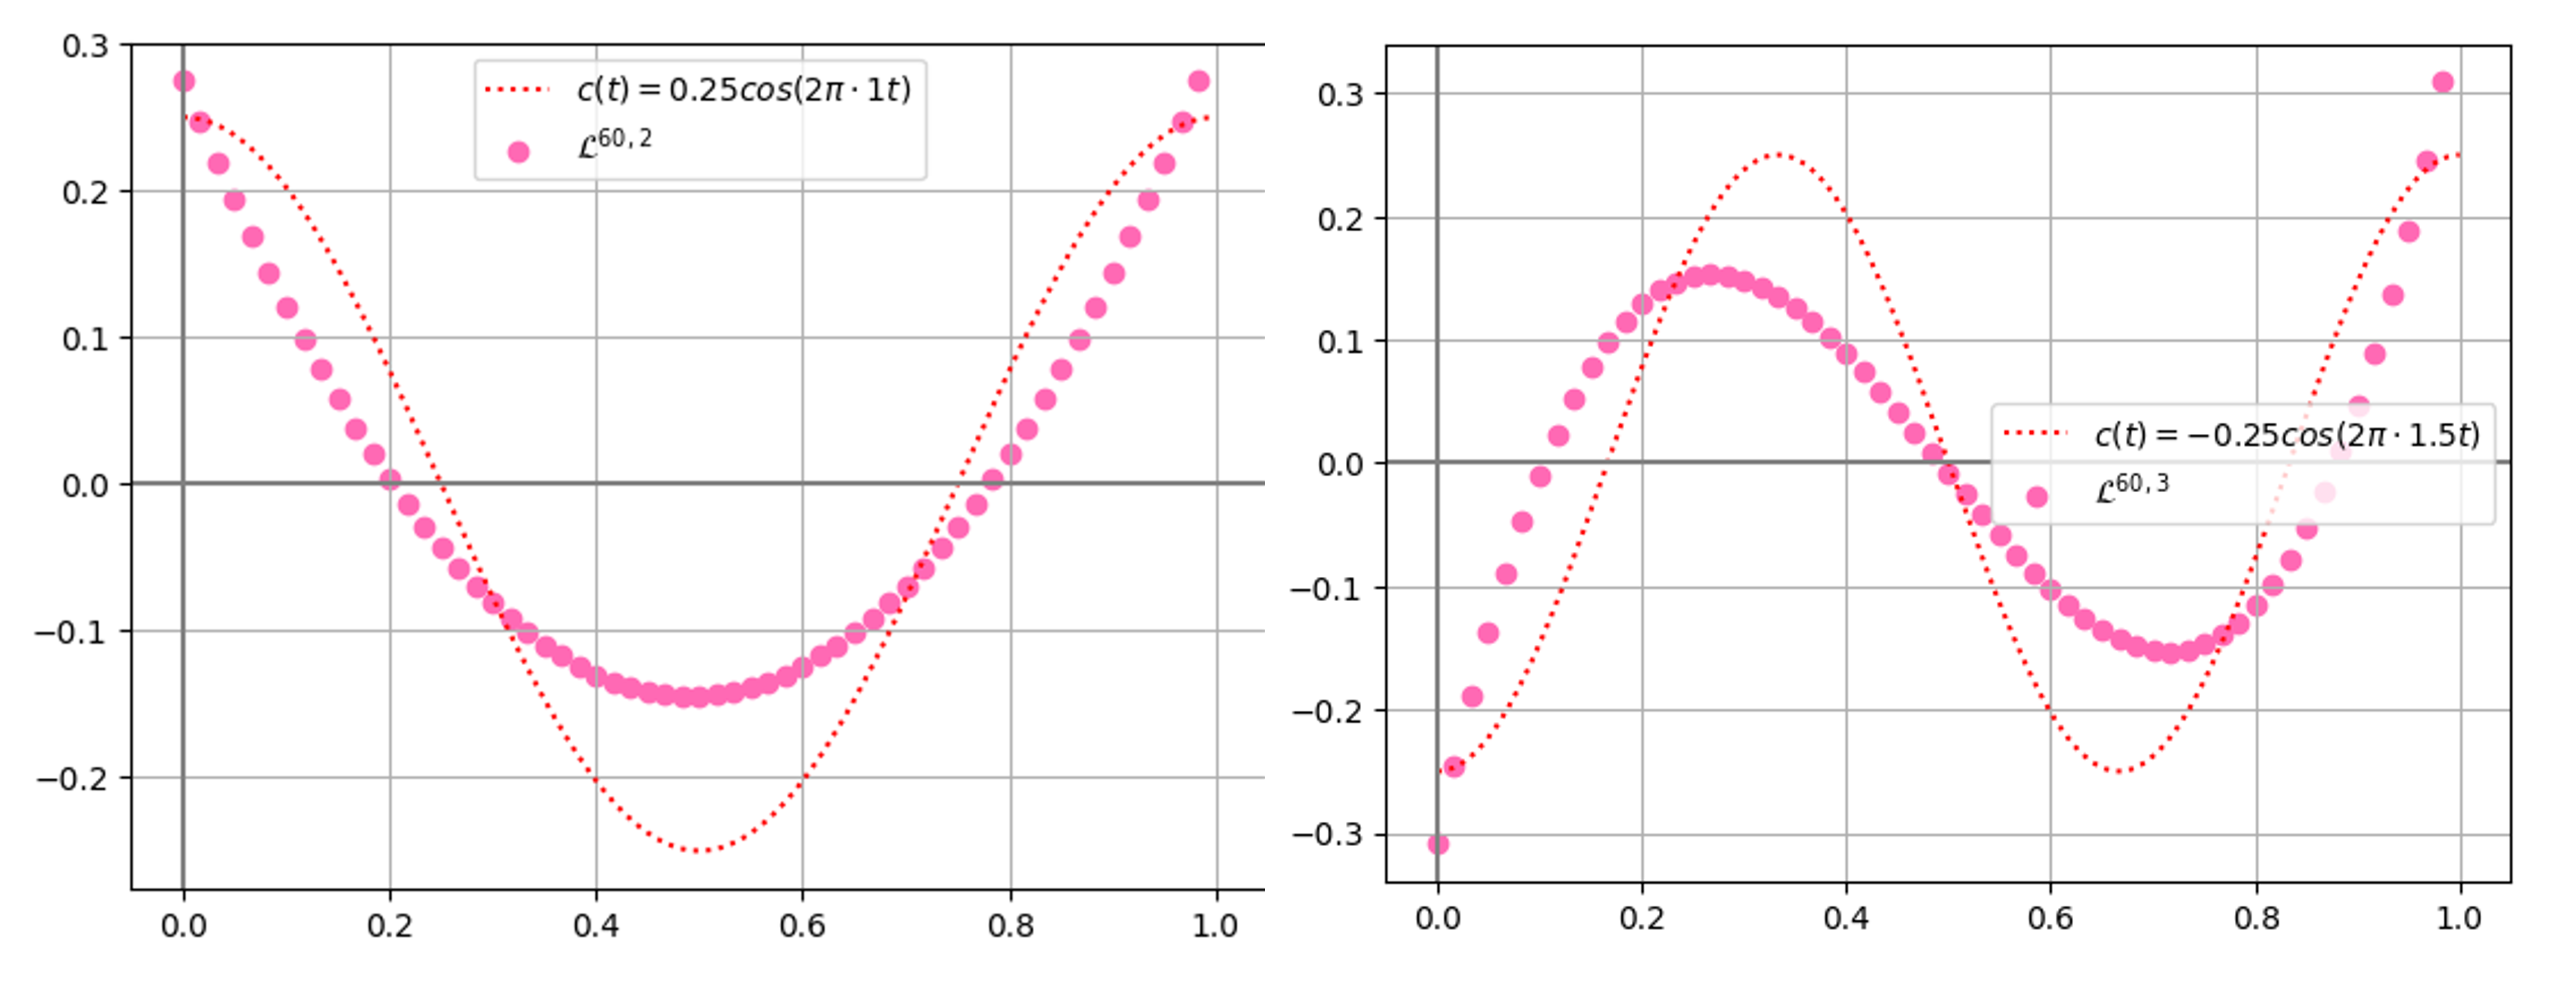
\includegraphics[scale = 0.6]{hip_2,3} 
\end{figure}	

\begin{figure}[H]
	\sidecaption{
	Aproximando las gráficas
	de $\cali{L}^{60,4}$ y $\cali{L}^{60,5}$
	con sinusoides. 
	\label{fig: hip_4,5}
	}
	\centering
	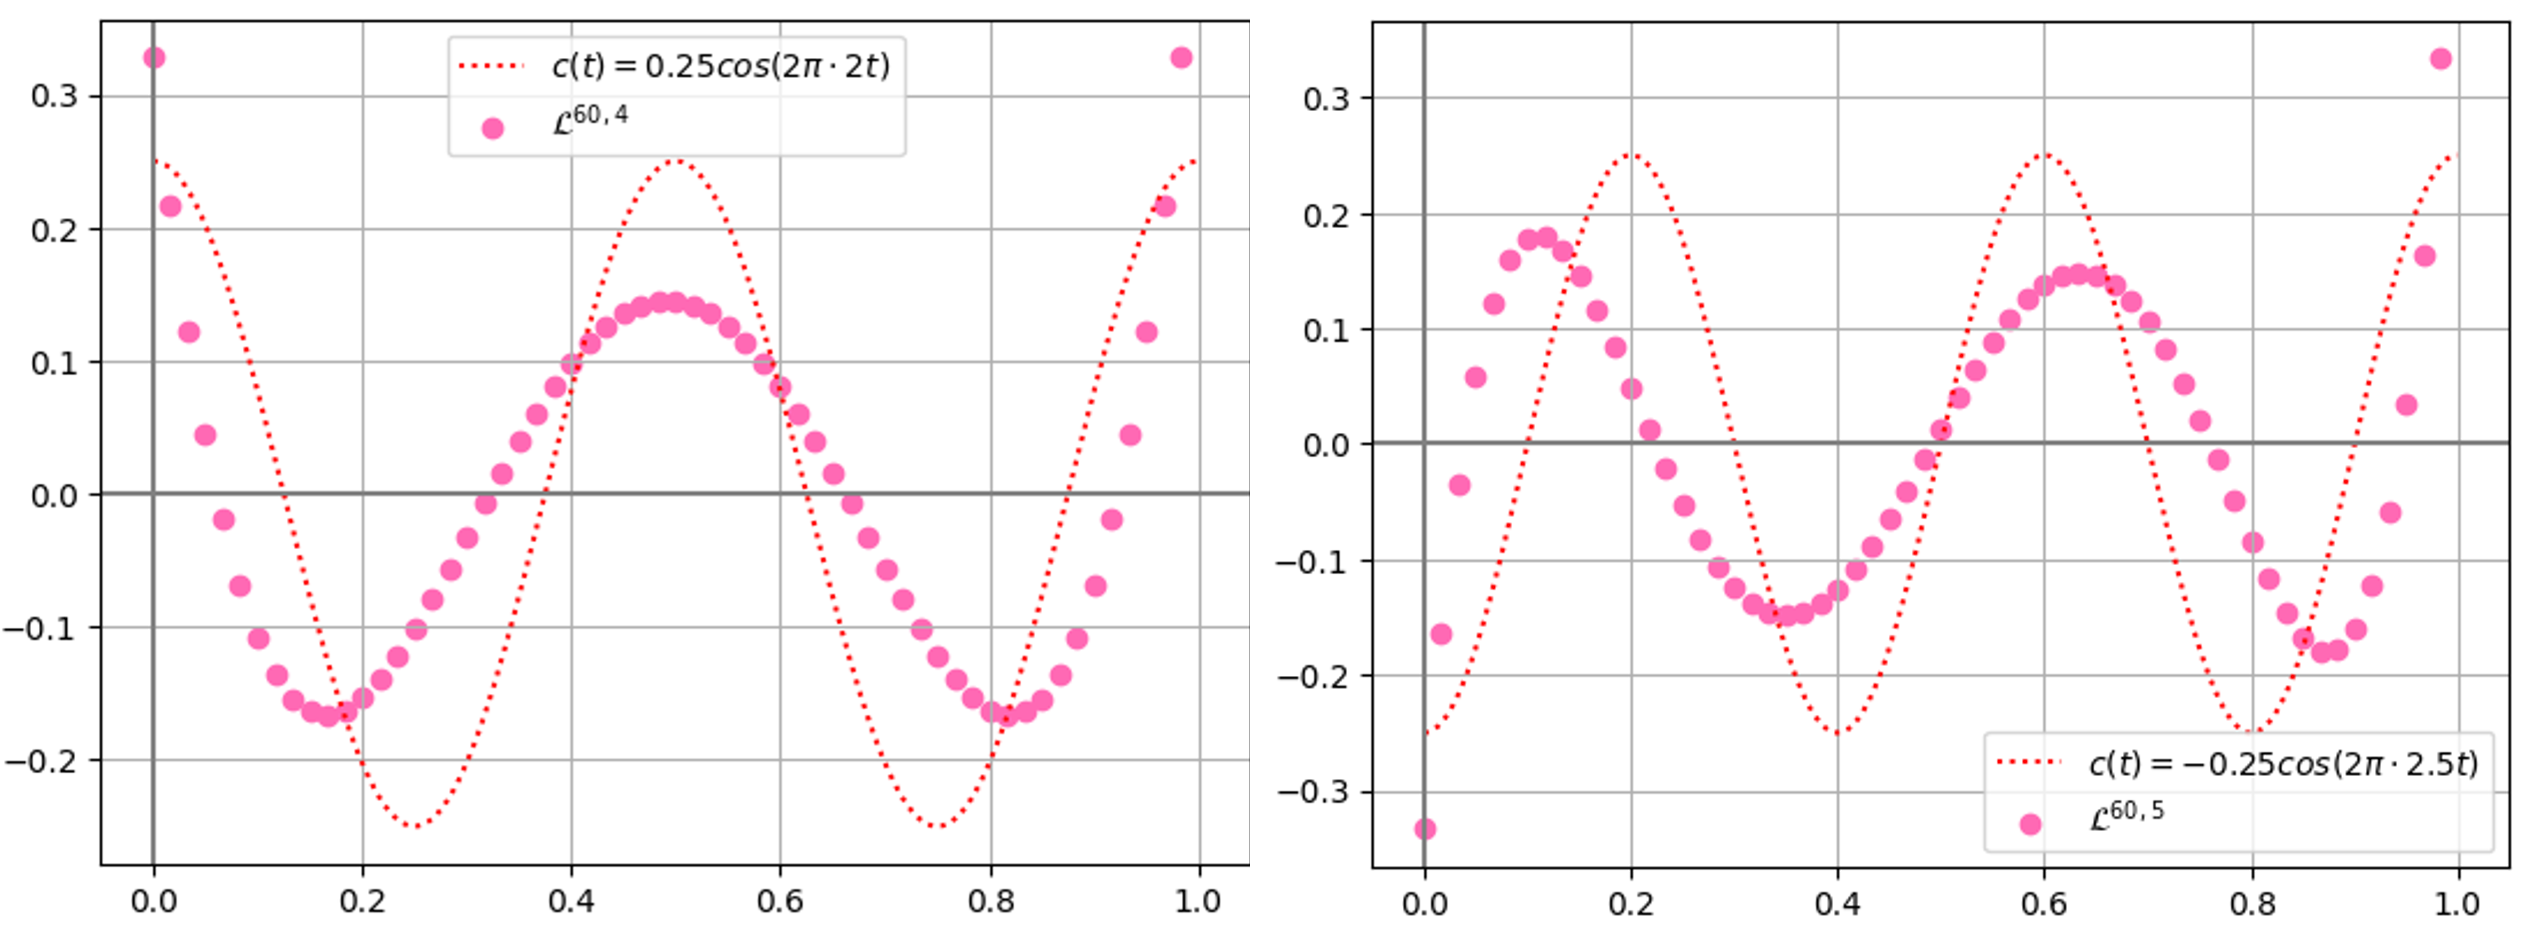
\includegraphics[scale = 0.6]{hip_4,5} 
\end{figure}	


Después de dibujar gráficas parecidas para varias dimensiones, 
establecemos la siguiente hipótesis de trabajo.

\begin{hip}
\label{ref: hipotesis}
Sean $n \geq 2$, $0 \leq k \leq n-1$ entero. 
Sea $\cali{L}^{n,k}$ el PDL de dimensión $n$ y grado $k$.
El espectro de $\cali{L}^{n,k}$ se concentra alrededor
de la frecuencia $\omega = k/2$.
\end{hip}

Se ha formulado de forma intencional la hipótesis 
\ref{ref: hipotesis} en términos vagos, para tener libertad
después de definir las herramientas con las que abordaremos el problema
de dar forma concreta a la hipótesis y mejorarla o refutarla con simulaciones
numéricas. \\ 

Observe que, para analizar la presencia de oscilaciones
en las gráficas de las señales, estamos hablando de un ``espectro''.
se cuenta ya con una herramienta clásica para hacer esta clase de análisis,
cuyo producto final es 
una función que
da información sobre
la importancia que cierta frecuencia tiene para
modelar la gráfica analizada. Hablamos de la transformada 
discreta de Fourier, cuyas bases teóricas comentamos en la sección
\ref{sec: TDF},
para usarla posteriormente para hacer un primer análisis espectral. Motivados
por algunas limitaciones de esta herramienta que comentamos más adelante,
nosotros proponemos una alternativa de metodología para realizar un análisis espectral 
en la sección 
\ref{sec: metodologia para realizar un analisis espectral que considere frecuencias arbitrarias}.

Algunos de los espectros así obtenidos se imprimen en
el capítulo
\ref{chap: resultados numericos analisis espectrales}.
El código para calcular tales espectros para cualquier
señal de $\IR^{n}$ se comparte en
\TODO{referencia cuaderno jupyter.}


\section{La transformada discreta de Fourier}
\label{sec: TDF}

En esta sección vamos a dar la definición usual de 
las bases de Fourier complejas y reales, que son
bases ortonormales de $\IC^{n}$ y de $\IR^{n}$ 
\marginnote{Incluimos este capítulo de teoría clásica
por completitud de este trabajo
y para fijar la notación. 
\cite{fourier1} y \cite{fourier2}
son referencias con mucha más información.}
de $\IC^{n}$
y una de $\IR^{n}$ (que llamaremos
``bases de Fourier complejas y reales''),
definidas ambas en términos de discretizaciones de
sinusoides de frecuencias enteras, y que son herramientas
clásicas para hacer lo que comúnmente se denomina
un \textbf{análisis espectral} de señales finitas.


Puesto que la definición de estas herramientas requiere
de algunas nociones del análisis complejo (en particular, de la
definición de la exponencial compleja y de las raíces $n-$ésimas
de la unidad), damos brevemente algunas definiciones y resultados
necesarios para definir las bases de Fourier.


\subsection{La exponencial compleja y raíces $n-$ésimas de la unidad}


La definición de la función exponencial compleja 
tiene diversas motivaciones
(puede consultar algunas de estas en 
\cite{marsden}). Nosotros sólo
damos la definición de esta, así como algunas propiedades
de ella que se usarán en lo que sigue.

\begin{defi}
\label{def: exponencial compleja}
Si $y \in \IR$, entonces por $exp(iy)$ denotamos al número
complejo de módulo uno y argumento $y$, es decir,
\begin{equation}
\label{eq: exponencial 1}
exp(iy) := cos(y) + i sen(y).
\end{equation}
Para todo número complejo $z = a+bi$, definimos 
$exp(z)$ como sigue:
\begin{equation}
\label{eq: exponencial 2}
exp(z) := e^{x}(cos(y) + i sen(y)).
\end{equation}
\end{defi}

\begin{prop}
\label{prop: propiedades exp compleja}
(\textbf{Algunas propiedades de la exponencial compleja}) 
Sean $z_{1}, z_{2} \in \IC$, $\omega \in \IZ$.
	\begin{itemize}
	\item $\frac{exp(z_{1})}{exp(z_{2})} = exp(z_{1} - z_{2})$
	\item $exp(z_{1} + z_{2}) = exp(z_{1}) \cdot exp(z_{2})$
	\item $(exp(z_{1}))^{\omega} = exp(\omega z)$
	\item $exp(z) = 1$ si y sólo si $z= 2K \pi i$ para algún $K \in \IZ$ 
	\item para todo $y \in \IR$, 
	\begin{equation}
	\label{eq: coseno exponenciales}
	cos(y) = \frac{exp(iy)+exp(-iy)}{2}
	\end{equation}
	y
	\begin{equation}
	\label{eq: seno exponenciales}
	sen(y) = \frac{exp(iy)-exp(-iy)}{2i}.
	\end{equation}
	\end{itemize}
\end{prop}

\begin{defi}
\label{defi: raices n esimas de la unidad}
Sea $n \in \IN$. A las $n$ raíces complejas del polinomio
$p_{n}(t)= t^{n}-1 \in \IC[t]$ 
se les denominará las \textbf{raíces $n-$ésimas de la unidad.}
\end{defi}


Las raíces $n-$ésimas de la unidad son pues los números complejos
tales que, elevados a la potencia $n$, son iguales a 1; según el 
teorema fundamental
del álgebra \ref{teo: fundamental del algebra}, sí hay números complejos
que satisfacen la definición \ref{defi: raices n esimas de la unidad}, y además
son a lo más $n$. Es fácil establecer, como hacemos a continuación, 
fórmulas explícitas para estos números, que de hecho son exactamente $n$.

\begin{prop}
Sea $n \in \IN$, $n \geq 2$. Hay exactamente $n$ raíces $n-$ésimas de la
unidad, y estas son los números complejos
 	\begin{equation}
	\label{eq3: 8ab}
	z_{n, \omega} : = exp \left( \frac{2 \pi i }{n} \omega
	\right), \hspace*{0.2cm} \textit{con} 
	\hspace*{0.2cm} \omega \in \{0, 1, \ldots, n-1 \}.
	\end{equation}
	
\end{prop}
\noindent
\textbf{Demostración.}
Por las propiedades expresadas en la proposición
\ref{prop: propiedades exp compleja}, es fácil ver que 
$z_{n,1} :=  exp \left( \frac{2 \pi i }{n} \right)$ es raíz $n-$ésima
de la unidad, pues
\[
(z_{n,1})^{n} = exp(2 \pi i ) = 1.
\]
Además, para todo $\omega \in \{ 0, \cdots , n-1 \}$, el número
\[
z_{n, \omega} : = (z_{n,1})^{\omega} = exp \left( \frac{2 \pi i }{n} \omega \right)
\]
también es es raíz $n-$ésima de la unidad, ya que

\[
(z_{n, \omega})^{n} = ((z_{n,1})^{\omega} )^{n} = 
((z_{n,1})^{n} )^{\omega} = 1^{\omega}=1. 
\]
Note ahora que los $n$ números complejos $z_{n, \omega}$ son todos 
distintos entre sí, pues si $\omega_{1}$ y $\omega_{2}$ son enteros
entre $0$ y $n-1$ tales que $z_{n, \omega_{1}} = z_{n, \omega_{2}}$,
o sea, tales que 
$exp \left( \frac{2 \pi i }{n} \omega_{1} \right) = 
exp \left( \frac{2 \pi i }{n} \omega_{1} \right)$, entonces, según el primer
punto de la proposición \ref{prop: propiedades exp compleja},
$1 = exp \left( \frac{2 \pi i }{n} (\omega_{1}-\omega_{2}) \right)$, luego, 
según el cuarto punto de esta misma proposición, $\frac{\omega_{1}-\omega_{2}}{n}$
es entero, o sea, $n$ divide a $\omega_{1}-\omega_{2}$; por el rango de 
$\omega_{1}$ y $\omega_{2}$, esto sólo ocurre si $\omega_{1}-\omega_{2}$ es
cero, o sea, si $\omega_{1}$ y $\omega_{2}$
son iguales.
\QEDB
\vspace{0.2cm}

\begin{figure}[H]
	\sidecaption{
	Para construir gráficamente a las raíces $n-$ésimas de la
	unidad, se debe dividir, a partir del punto $(0,1)$, a la
	circunferencia unitaria en $n$ partes iguales. Según esta construcción
	y la interpretación geométrica de la multiplicación compleja, es claro
	que multiplicando a $z_{n,1}$ consigo mismo se obtienen a
	todas las demás raíces $n-$ésimas.
	\label{fig: raices unidad}
	}
	\centering
	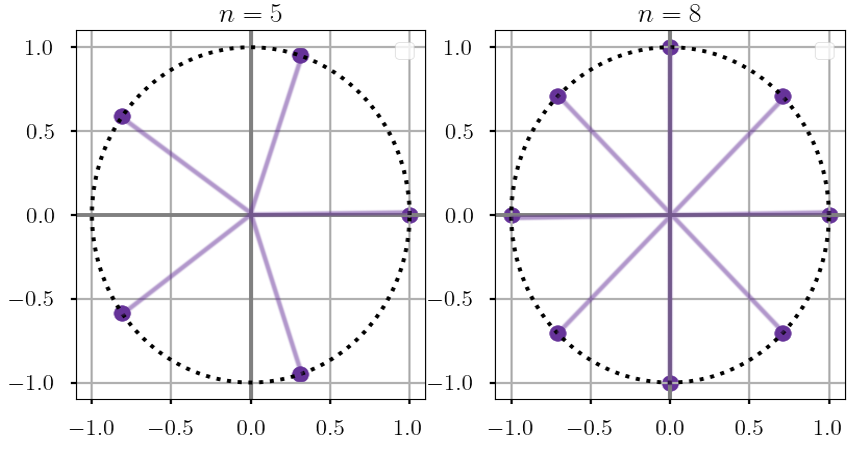
\includegraphics[scale=0.53]{raices_unidad} 
\end{figure}	


\subsection{La transformada discreta de Fourier}

Ya tenemos todo lo necesario para definir a la base
de Fourier compleja de la que hablamos al inicio.
\marginnote{El producto punto que estamos
considerando en el $\IC-$espacio
vectorial $\IC^{n}$ es el que definimos
en \eqref{eq: producto punto Cn}, y el del
$\IR-$espacio vectorial $\IR^{n}$ es el definido en 
\eqref{eq: producto punto Rn}.}

\begin{prop}
\label{prop: construccion Bn}
Sea $n \in \IN$. El conjunto

\begin{equation}
\label{eq2: 8ab}
\cali{B}_{n} : = \left\{
e_{n,\omega} = \left(
\frac{1}{\sqrt{n}} exp \left(
2 \pi i \omega \frac{m}{n}
\right)
\right)_{0 \leq m \leq n-1}
: \hspace{0.2cm} 0 \leq \omega \leq n-1
 \right\}
\end{equation}
es una base ortonormal del $\IC-$espacio
vectorial $\IC^{n}$.
\end{prop}

\noindent
\textbf{Demostración.}
Calculemos el producto punto de dos elementos
$e_{n,\omega_{1}}$ y $e_{n,\omega_{2}}$ del conjunto \eqref{eq2: 8ab};
si $\omega := \omega_{1}-\omega_{2}$,
\begin{align*}
\langle e_{n,w_{1}}, e_{n,w_{2}} \rangle = &
\frac{1}{n}
\suma{m=0}{n-1}{exp \left( 2 \pi i \frac{m}{n} \omega_{1} \right)
\cdot \overline{ exp \left( 2 \pi i \frac{m}{n} \omega_{2} \right) }} \\
= & \frac{1}{n}
\suma{m=0}{n-1}{\left( 2 \pi i \frac{m}{n} (\omega_{1}-\omega_{2}) \right)} \\
= & \frac{1}{n}\suma{m=0}{n-1}{exp\left( 2 \pi i \frac{\omega}{n} m \right)} \\
= & \frac{1}{n}\suma{m=0}{n-1}{exp\left( 2 \pi i \frac{\omega}{n}  \right)^{m}} \\
= & \frac{1}{n}\suma{m=0}{n-1}{(z_{n, \omega})^{m}};
\end{align*}

\noindent
esta última es una suma geométrica. 
\begin{itemize}
	\item Si $\omega_{1} \neq \omega_{2}$, entonces $n$ no puede dividir 
	a $\omega = \omega_{1}-\omega_{2}$ (pues, por el rango en el que se encuentran
	$\omega_{1}$ y $\omega_{2}$, $w \in [-(n-1), n-1]$, y el único múltiplo
	de $n$ en este intervalo es cero), luego, $z_{n, \omega} \neq 1$.
	En este caso se tiene entonces que 
	\[
	\langle e_{n,w_{1}}, e_{n,w_{2}} \rangle = 
	\frac{1}{n}\suma{m=0}{n-1}{(z_{n, \omega})^{m}}
	= \frac{1}{n} \cdot \frac{(z_{n, \omega})^{n}-1}{z_{n, \omega}-1}=
	\frac{1}{n} \cdot \frac{1-1}{z_{n, \omega}-1}=0.
	\]
	
	\item Si $\omega_{1} = \omega_{2}$, entonces $\omega = 0$, y
	\[
	\langle e_{n,w_{1}}, e_{n,w_{2}} \rangle = 
	\frac{1}{n}\suma{m=0}{n-1}{(z_{n, 0})^{m}}
	= \frac{1}{n}\suma{m=0}{n-1}{1} = \frac{1}{n} \cdot n = 1.
	\]
\end{itemize}

Demostramos así que los elementos de $\cali{B}_{n}$
tienen norma uno y que además
son ortogonales
dos a dos, luego, $\cali{B}_{n}$ es un subconjunto l.i. 
de $\IC^{n}$; como $\IC^{n}$ es un $\IC-$espacio vectorial de 
dimensión $n$, concluimos lo deseado.
\QEDB
\vspace{0.2cm}

Por ser \eqref{eq2: 8ab} una BON de $\IC^{n}$, siempre es
posible expresar a un vector $x = (x_{m})_{0 \leq m \leq n-1} \in \IC^{n}$
como combinación lineal de los elementos de \eqref{eq2: 8ab}
y además los coeficientes están dados por los productos punto
de $x$ y los elementos de \eqref{eq2: 8ab}
(c.f. nota \ref{nota: sobre la identidad de parseval}).

\begin{defi}
Sean $n \in \IN$, $x = (x_{m})_{m=0}^{n-1} \in \IC^{n}$
una señal compleja de longitud $n$.
Sea $\cali{B}_{n}$ la base de $\IC^{n}$ definida en 
la proposición \ref{prop: construccion Bn}. \\

A la función $f_{x}: \{ 0, 1, \ldots, n-1 \} 
\rightarrow \IC^{n}$ que a cada
frecuencia $\omega \in \{ 0, 1, \ldots, n-1 \} $
le asocia el coeficiente de $x$ respecto 
al elemento $e_{n, \omega}$ de la base
$\cali{B}_{n}$, o sea, la función definida como
\begin{equation}
\label{eq: TDF}
f_{x}(\omega) = X_{\omega} := 
\frac{1}{\sqrt{n}} \suma{m=0}{n-1}{x_{m} exp \left(
2 \pi i \omega \frac{m}{n}
\right)}
\end{equation}
le llamaremos la 
\textbf{transformada discreta de Fourier de $x$}.
Muchas veces identificamos a tal transformada
con el vector
$X := (X_{\omega})_{\omega = 0}^{n-1}$, que 
no es más que la representación 
de $x = (x_{m})_{m=0}^{n-1}$ respecto a la 
base de frecuencias $\cali{B}_{n}$.
\end{defi}

\marginnote{Por sus siglas en inglés, a la transformada discreta
de Fourier también se le denomina ``TDF''.}


\begin{comment}
{\Huge{\textcolor{red}{TDF}}} 

{\Huge{\textcolor{red}{Dominio: tiempo}}} 


{\Huge{\textcolor{red}{Dominio: frecuencia}}}

{\Huge{ $x = (x_{m})_{0 \leq m \leq n-1}$ }}

{\Huge{ $\langle x, e_{\omega} \rangle$, $0 \leq \omega \leq n-1 $ }}

\end{comment}

Calcular entonces la transformada discreta de Fourier
de $x$ consiste en calcular a los productos
punto $\langle x, e_{n,\omega} \rangle $, que son

\begin{align*}
X_{\omega} := \langle x, e_{n,\omega} \rangle = & 
\frac{1}{\sqrt{n}} \suma{m=0}{n-1}{x_{m} exp \left(
2 \pi i \omega \frac{m}{n}
\right)} \\
= & 
\frac{1}{\sqrt{n}} \suma{m=0}{n-1}{x_{m} 
\left(
exp \left( \frac{2 \pi i }{n} \omega
\right) \right)^{m}} \\
= & A_{x}(z_{n, \omega}),
\end{align*}


\noindent
donde $z_{n, \omega}$ es como en \eqref{eq3: 8ab} y 
$A_{x} = A_{x}(t) \in \IC[t]$ es el polinomio de 
coeficientes complejos definido 
a partir de $x$ como sigue:

	\begin{equation}
		\label{eq4: 8ab}
		A_{x}(t) := \suma{m=0}{n-1}{\frac{x_{m}}{\sqrt{n}} t }\in \IC[t];
	\end{equation}

\noindent
así, \textbf{calcular la transformada
discreta de Fourier de $x$ es lo mismo que evaluar al polinomio 
$A_{x}$ de grado a lo más $n-1$ definido en \eqref{eq4: 8ab} en todas las raíces
$n-$ésimas de la unidad.} 


\begin{nota}
Según este último párrafo, calcular transformadas discretas
de Fourier requiere de algoritmos eficientes para evaluar
polinomios en raíces $n-$ésimas de la unidad. Usando propiedades
de las raíces $n-$ésimas de la unidad (por ejemplo,
véase el lema 30.5 de \cite{algorithms}) 
es posible usar recursión para disminuir
el tiempo de cómputo. Al algoritmo estándar usado para
esto se le conoce como la \textbf{transformada rápida de 
Fourier} (abreviado como ``FFT'' por sus siglas en inglés);
puede consultar los detalles técnicos en el capítulo
30 de \cite{algorithms}.
\end{nota}

\begin{nota}
Se calcula fácilmente una fórmula para la 
inversa de la transformada discreta de Fourier 
$f_{x}$ de una señal $x$; si
se conoce la TDF $X = (X_{\omega})_{\omega=0}^{n-1}$
de una señal $x \in \IC^{n}$, pueden recuperarse sus coeficientes
respecto a la base canónica de $\IC^{n}$ (i.e. su representación
respecto al tiempo)
como sigue:
\begin{equation}
\label{eq: TDFI}
\forall \hspace{0.1cm} 0 \leq m \leq n-1:
\hspace{0.2cm}
x_{m} = \frac{1}{\sqrt{n}} 
\suma{k=0}{n-1}{
X_{k} exp \left( 
-2 \pi i k \frac{m}{n}
\right).
}
\end{equation}

En ocasiones, por transformada discreta de Fourier y su 
inversa se toman las opuestas a las que hemos definido aquí
(i.e. se pide el signo negativo en la exponencial 
para la TDF y se toma el signo positivo para la inversa); además,
se toman distintos factores de normalización
(por ejemplo, $1$ para la TDF y $\frac{1}{n}$ para la
inversa), c.f. \cite{TDFwiki}. Puede ver que fórmulas
para la TDF y su inversa son implementadas en el 
módulo \texttt{scipy.fft} de Python con las modificaciones descritas
antes (puede consultar la documentación de esta librería en
\cite{FFTscipy}).
\end{nota}

\begin{figure}[H]
\centering\captionsetup{format = hang}
	\begin{measuredfigure}
		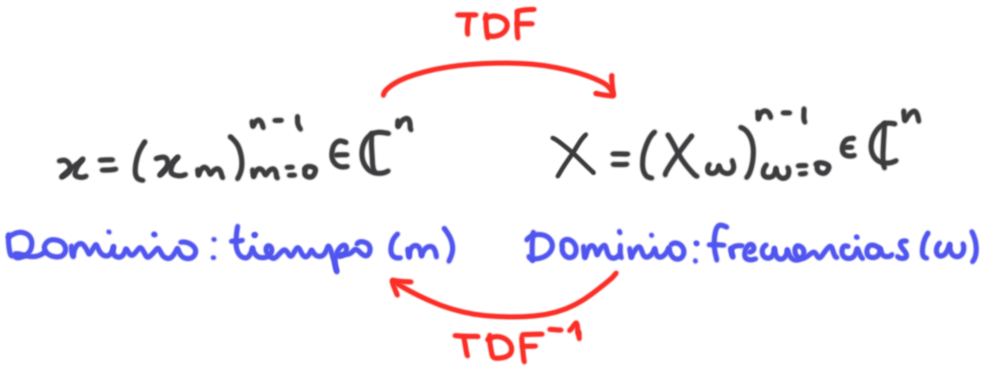
\includegraphics[scale=1.35]{tiempo_freq.png} 
		\caption{Usualmente uno representa a una señal discreta
		$x$ de dimensión $n$ con $n$ mediciones complejas; en este caso, el dominio
		de la representación es el tiempo. Pero
		también se puede representar unívocamente a $x$ con sus
		coeficientes respecto a la base de frecuencias 
		$\cali{B}_{n}$; en este caso, puesto que cada coeficiente da
		el peso que tiene la respectiva frecuencia para construir la 
		señal original $x$, decimos que el dominio de la representación
		es el de frecuencia. Las fórmulas para pasar de una
		representación a otra son \eqref{eq: TDF} y \eqref{eq: TDFI}.}
 	\end{measuredfigure}
\end{figure}


Al usar a $\cali{B}_{n}$ como sistema de representación en
$\IC^{n}$, lo que estamos haciendo es representar a
un $x = (x_{m})_{0 \leq m \leq n-1}$ como combinación
lineal de los vectores 

\[
e_{n,\omega} = \frac{1}{\sqrt{n}} \left( cos
\left( 2 \pi \omega \frac{m}{n} \right)
+ i sen \left( 2 \pi \omega \frac{m}{n}\right) \right)_{0\leq m \leq n-1},
\hspace{0.2cm} 0 \leq \omega \leq n-1;
\]
observe que las partes reales de las
entradas de $e_{n,\omega} \in \IC^{n}$ se obtienen de tomar $n$
muestras uniformes de la función 
$c_{\omega}(t) := \frac{1}{\sqrt{n}} cos (2 \pi \omega t)$ (o sea, de la función
coseno de amplitud $\frac{1}{\sqrt{n}}$, frecuencia $\omega$ y desfase $0$)
y, similarmente,
las partes imaginarias de las entradas se obtienen muestreando
uniformemente a la función 
$s_{\omega}(t) := \frac{1}{\sqrt{n}}  sin (2 \pi \omega t)$.

\begin{figure}[H]
	\sidecaption{
	Por ejemplo, si $n=5$, para construir al vector
	$e_{3}$ de la base $\cali{B}_{n}$ se muestrean uniformemente
	cosenos y senos de frecuencia $3$ como se muestra en la figura;
	los puntos rojos representan las partes reales de las entradas
	y los azules las imaginarias.
	\label{fig: construccion Bn}
	}
	\centering
	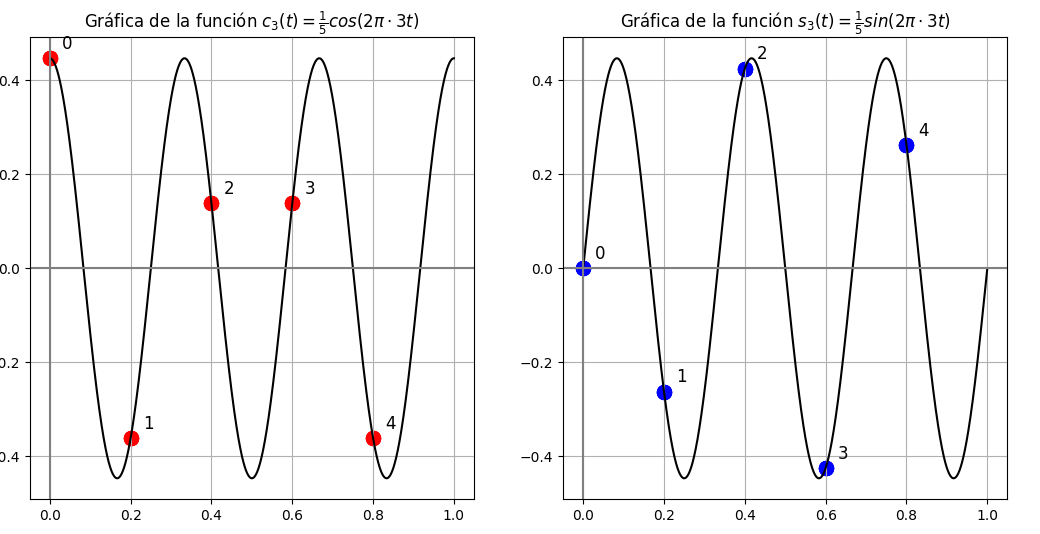
\includegraphics[scale=0.29]{construccion_Bn} 
\end{figure}	

Según esto, el vector $e_{n,\omega}$ se construye a partir
de funciones de frecuencia $\omega$; considerando esto
y el que $\cali{B}_{n}$ sea una BON de $\IC^{n}$ (luego, el
que se valga la identidad de Parseval,
c.f. nota \ref{nota: sobre la identidad de parseval}), tenemos que
la síntesis

\[
x = \suma{\omega=0}{n-1}{\langle x, e_{n,\omega} \rangle e_{n,\omega}}
\]

\noindent
es una expresión de $x$ en términos de vectores de frecuencia
$\omega$ y que los respectivos coeficientes 
$\langle x, e_{n,\omega} \rangle$ indican qué tanto 
contribuye la frecuencia $\omega$ para construir a $x$.

Es por eso que al proceso de considerar representaciones
de señales complejas finitas respecto a las bases de Fourier
se le conoce como  
\textbf{realizar un análisis espectral.}


\subsection{Versión real de la TDF}

En el caso en el que todas las entradas de un vector
$x = (x_{m})_{0 \leq m \leq n-1}$ sean reales, se puede definir
una base ortonormal de $\IR^{n}$, 
análoga a la BON $\cali{B}_{n}$ de $\IC^{n}$ construida en 
\ref{prop: construccion Bn},
a partir de muestreos uniformes
de sinusoides de frecuencias enteras.

\begin{prop}
\label{prop: base de fourier version real}
Sean $n \in \IN$ mayor a uno, $M = \lceil \frac{n}{2} \rceil$.
Definimos a los vectores de $\IR^{n}$

\[
c_{n, 0}= \left( \sqrt{\frac{1}{n}} cos
	\left(2 \pi \cdot 0 \frac{m}{n}
	\right) \right)_{m=0}^{n-1} = 
	\left( \frac{1}{\sqrt{n}}, \cdots, \frac{1}{\sqrt{n}} \right),
\]

	\begin{equation}
	\label{eq0: 10ab}
	c_{n, \omega} := \left( \sqrt{\frac{2}{n}} cos
	\left(2 \pi \omega \frac{m}{n}
	\right) \right)_{m=0}^{n-1},
	\hspace{0.2cm} 1 \leq \omega \leq M-1
	\end{equation}
	
	\begin{equation}
	\label{eq0: 4May}
	s_{n, \omega} := \left( \sqrt{\frac{2}{n}} sin
	\left(2 \pi \omega \frac{m}{n}
	\right) \right)_{m=0}^{n-1},
	\hspace{0.2cm} 1 \leq \omega \leq M-1
	\end{equation}
	
y, en el caso en que n sea par, definimos también
al vector

	\[
c_{n, M}= \left( \sqrt{\frac{1}{n}} cos
	\left(2 \pi \cdot M \frac{m}{n}
	\right) \right)_{0 \leq m \leq n-1} = 
	\left( \frac{(-1)^{m}}{\sqrt{n}} \right)_{m=0}^{n-1}.
\]

El subconjunto $\cali{F}_{n}$ de $\IR^{n}$ definido como

	\begin{itemize}
	\item $\cali{F}_{n} : = \{ c_{n,0}, c_{n,1}, s_{n,1},
	\ldots , c_{n,M-1}, s_{n,M-1}, c_{n,M} \}$ si $n$ es par
	(o sea, si $n=2M$), y como
	\item $\cali{F}_{n} : = \{ c_{n,0}, c_{n,1}, s_{n,1},
	\ldots , c_{n,M-1}, s_{n,M-1} \}$ si $n$ es impar
	(o sea, si $n=2M-1$)
	\end{itemize}
	
es una base ortonormal del $\IR-$espacio vectorial $\IR^{n}$.
\end{prop}

\noindent
\textbf{Demostración.}
Supongamos $n$ par. Si $0 \leq \omega_{1}, \omega_{2} \leq M$
son enteros, entonces
$\omega_{1} + \omega_{2}$ sólo es divisible por $n$ si ambos números
son iguales a $M$. Si suponemos a $\omega_{1}$ y $\omega_{2}$ distintos, 
entonces

\begin{align*}
\langle c_{n, \omega_{1}} , c_{n, \omega_{2}} \rangle = &
\frac{1}{n} \suma{m=0}{n-1}{cos \left(2 \pi \omega_{1} \frac{m}{n} \right) \cdot 
cos \left(2 \pi \omega_{2} \frac{m}{n} \right)} \\
= &\frac{1}{2n} \left(
cos \left(2 \pi (\omega_{1} + \omega_{2}) \frac{m}{n} \right) +
cos \left(2 \pi (\omega_{1} - \omega_{2}) \frac{m}{n} \right)
\right) \\
= & \frac{1}{4n} (
\suma{m=0}{n-1}{
(exp(2 \pi m(\omega_{1}+\omega_{2})i/n) +
exp(-2 \pi m(\omega_{1}+\omega_{2})i) } \\
&  + exp(2 \pi m(\omega_{1}-\omega_{2})i/n) +
exp(-2 \pi m(\omega_{1}-\omega_{2})i)) )\\
\textit{(suma geométrica)} = & 
\frac{exp(2 \pi i (\omega_{1}+\omega_{2}))-1}{4n (exp(2 \pi i (\omega_{1}+\omega_{2})/n)-1)} +
\frac{exp(- 2 \pi i (\omega_{1}+\omega_{2}))-1}{4n (exp(-2 \pi i (\omega_{1}+\omega_{2})/n)-1)}
\\
& + 
\frac{exp(2 \pi i (\omega_{1}-\omega_{2}))-1}{4n (exp(2 \pi i (\omega_{1}-\omega_{2})/n)-1)} +
\frac{exp(- 2 \pi i (\omega_{1}-\omega_{2}))-1}{4n (exp(-2 \pi i (\omega_{1}-\omega_{2})/n)-1)};
\\
\end{align*}

\noindent
puesto que $\omega_{1}+\omega_{2}$ y $\omega_{1}-\omega_{2}$
son ambos enteros, según la proposición 
\ref{prop: propiedades exp compleja} las exponenciales de los numeradores
de esta última expresión son todas iguales a uno, luego, 
$\langle c_{n, \omega_{1}} , c_{n, \omega_{2}} \rangle  =0$. 


Con argumentos similares se prueba 
que todos los elementos de $\cali{F}_{n}$ tienen norma uno, así como
la ortogonalidad entre dos elementos
distintos del conjunto $\cali{F}_{n}$, por lo tanto, la independencia lineal de
este conjunto, luego, el que $\cali{F}_{n}$ sea base 
(ortonormal) de $\IR^{n}$.


\QEDB
\vspace{0.2cm}



\begin{defi}
Sea $n \in \IN$, $n \geq 2$. Llamaremos a la BON
$\cali{F}_{n}$ de $\IR^{n}$ definida en \ref{prop: base de fourier version real}
la \textbf{base de Fourier real de dimensión $n$}.
\end{defi}

\begin{nota}
\label{nota: frecuencias en las bases de fourier}
Observe que $\cali{F}_{n}$, a diferencia de $\cali{B}_{n} \subseteq \IC^{n}$, 
considera frecuencias enteras no mayores a $M := \lceil \frac{n}{2} \rceil$
(cuando $n$ es par) o a $M-1$ (cuando $n$ es impar), mientras que
en $\cali{B}_{n}$ se consideran las frecuencias enteras entre $0$
y $n-1$ (inclusivo); así, si decidimos representar
a una señal $x \in \IR^{n}$ en base a $\cali{F}_{n} \subseteq \IR^{n}$
y no en base a $\cali{B}_{n} \subseteq \IC^{n}$, sintetizaremos a $x$
respecto a frecuencias enteras acotadas por $M$ o por $M-1$ 
(dependiendo de la paridad de $n$), y no respecto a frecuencias
menores a $n$.
\end{nota}

\begin{ejemplo}
\label{ej: DFT1}
Consideremos a la señal 
\begin{equation}
\label{eq2: 10ab}
x=(-0.5,-8,-5.3,15,-0.3,6,4) \in \IR^{7}.
\end{equation}

Según la construcción de $\cali{F}_{7}$ (c.f. 
proposición \ref{prop: base de fourier version real}),
una expresión de $x$ respecto a $\cali{F}_{7}$ 
es una síntesis de $x$ a partir de señales 
de frecuencias $\omega = 0,1,2,3$. En la imagen de abajo
se muestran los coeficientes de $x$ respecto a $\cali{F}_{7}$.

\begin{figure}[H]
	\sidecaption{
	Se muestran la gráfica de $x$ junto con la gráfica de los
	coeficientes de $x$ respecto a la BON $\cali{F}_{7}$. Observe 
	que, por definición, sólo un vector de $\cali{F}_{7}$ tiene frecuencia
	cero (i.e. es constante), mientras que para las otras frecuencias
	tenemos dos vectores de la misma frecuencia, uno construido a partir de un 			
	coseno y otro a partir de un seno.
	\label{fig: ejFrecuencia 1}
	}
	\centering
	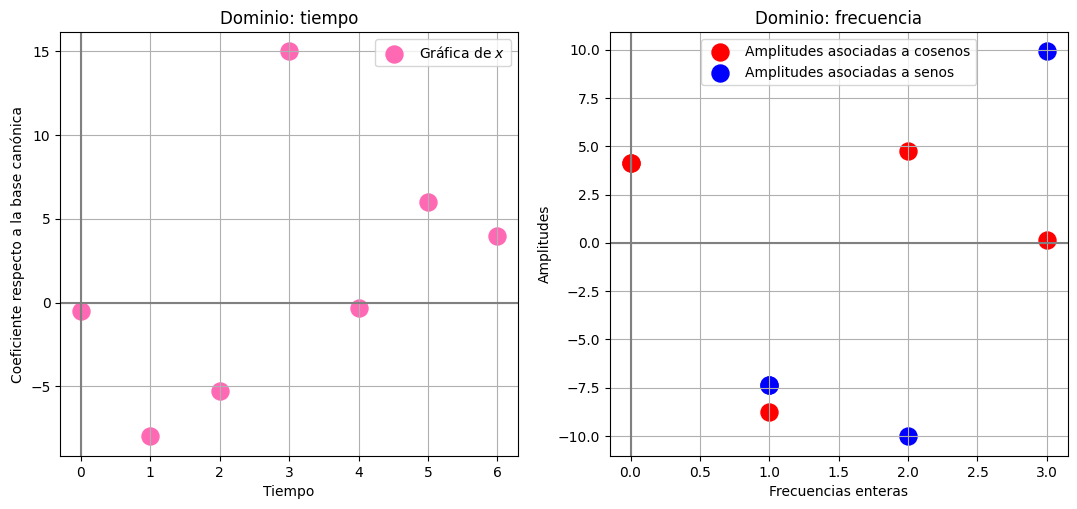
\includegraphics[scale=0.4]{ejFrecuencia_1} 
\end{figure}	

Redondeando los coeficientes, 
se tiene la siguiente descomposición de $x$;

\begin{equation}
\label{eq: analisis x TDF}
x = 4.12 c_{7,0} - 8.76c_{7,1} -7.35s_{7,1}+
4.77c_{7,2}-10s_{7,2}+0.14c_{7,3}+9.91s_{7,3}.
\end{equation}

\noindent
A continuación mostramos las gráficas
de los sinusoides que fueron discretizados
para obtener los vectores de frecuencia
$0,1,2$ y $3$ en los que descompusimos a $x$.

\begin{figure}[H]
	\sidecaption{
	Aporte de frecuencia $0$.
	\label{fig: ejFrecuencia 2}
	}
	\centering
	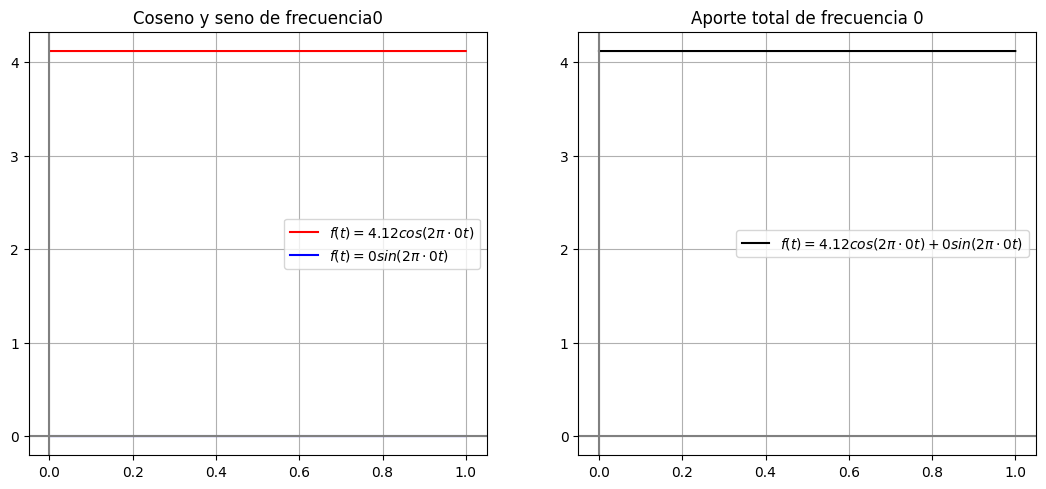
\includegraphics[scale=0.4]{ejFrecuencia_2} 
\end{figure}	

\begin{figure}[H]
	\sidecaption{
	Aporte de frecuencia $1$.
	\label{fig: ejFrecuencia 3}
	}
	\centering
	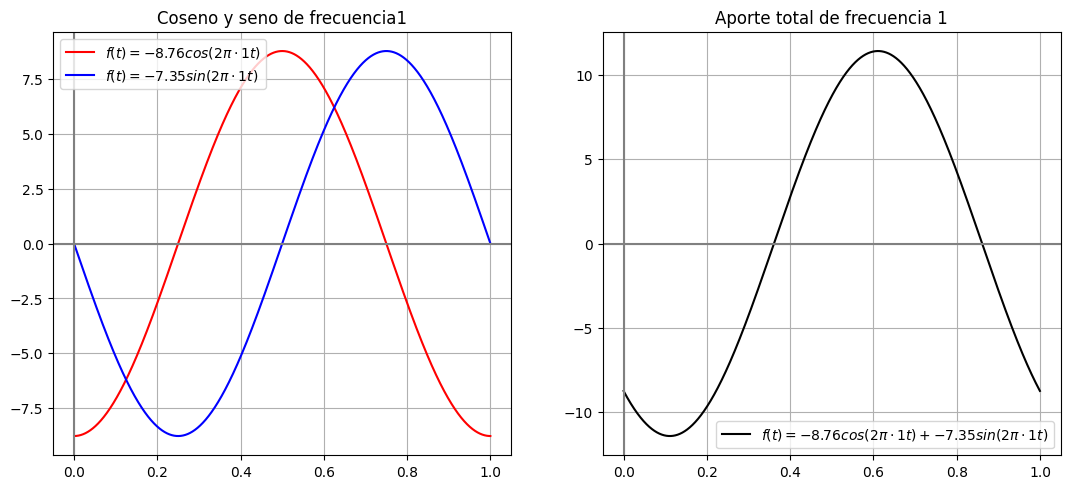
\includegraphics[scale=0.4]{ejFrecuencia_3} 
\end{figure}	

\begin{figure}[H]
	\sidecaption{
	Aporte de frecuencia $2$.
	\label{fig: ejFrecuencia 4}
	}
	\centering
	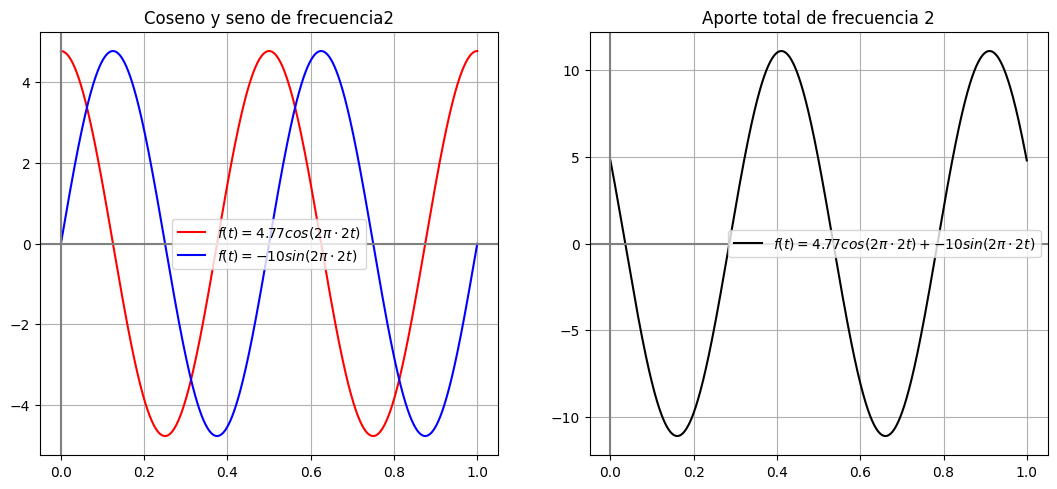
\includegraphics[scale=0.4]{ejFrecuencia_4} 
\end{figure}	


\begin{figure}[H]
	\sidecaption{
	Aporte de frecuencia $3$.
	\label{fig: ejFrecuencia 5}
	}
	\centering
	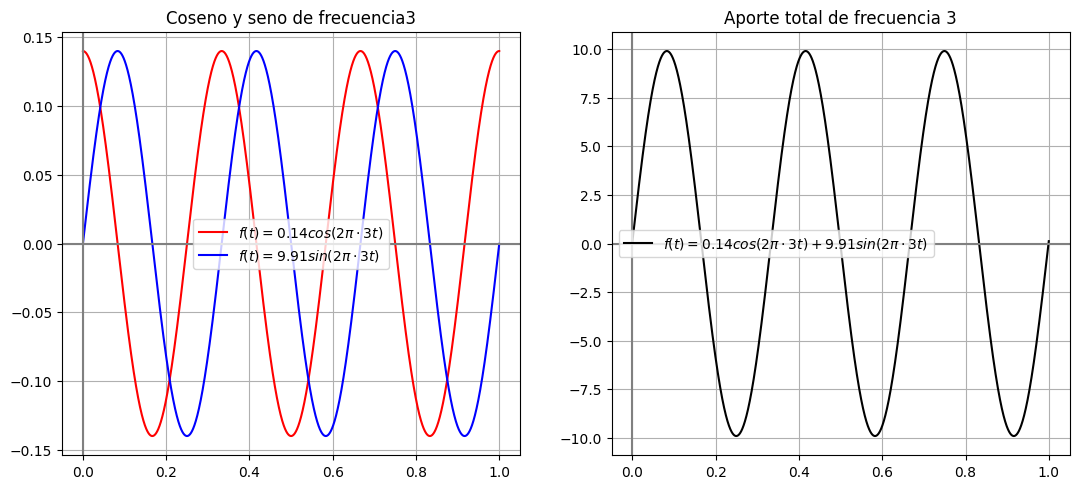
\includegraphics[scale=0.4]{ejFrecuencia_5} 
\end{figure}	

Sumando todas las gráficas de la derecha, obviamente
obtenemos una función de cosenos y senos tal que,
del muestrearla uniformemente en $[0,1]$, resulta
el vector $x$ \eqref{eq2: 10ab}.

\begin{figure}[H]
	\sidecaption{
	En morado se muestra la gráfica de la función suma
	de las gráficas derechas en las figuras anteriores.
	\label{fig: ejFrecuencia 6}
	}
	\centering
	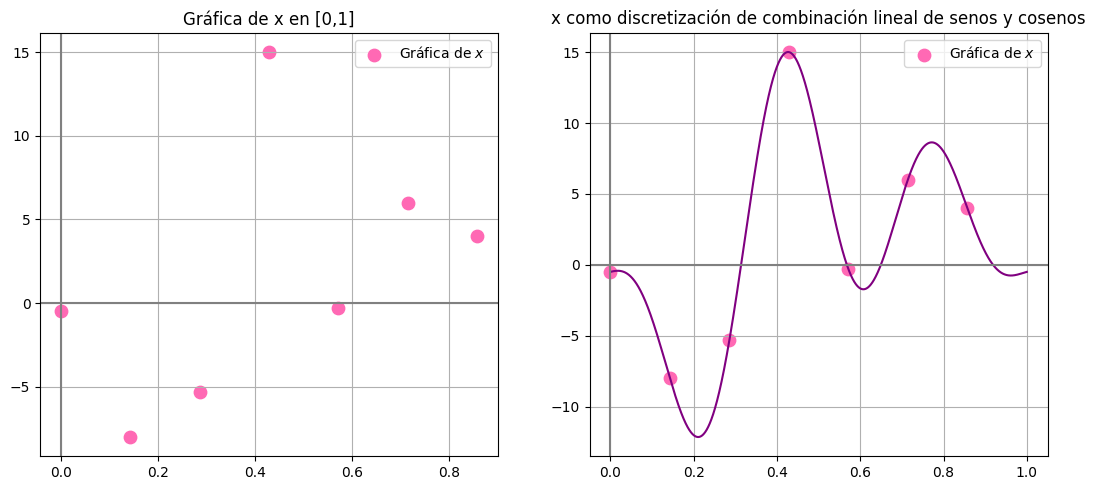
\includegraphics[scale=0.44]{ejFrecuencia_6} 
\end{figure}	
\final
\end{ejemplo}

Para terminar, digamos en concreto qué se entiende
por el espectro que resulta de usar la 
versión real de la transformada
discreta de fourier para analizar una señal finita.

En la definición 
$\cali{F}_{n}$ de la base dada en 
\ref{prop: base de fourier version real}, observe que, 
por cada frecuencia entera $\omega$ considerada,
aparecen uno o dos sinusoides (discretizados) con tal frecuencia:


\begin{table}[ht]
\sidecaption{Dimensión $n = 2M-1$ impar}
\centering
  \begin{tabular}{ l | c | c | c | c }
    \hline
    Frecuencia & $0$ & $1$ & $\ldots$ & $M-1$  \\ \hline
    Cant. sinusoides  & $1$ & $2$ & $\ldots$ & $2$ \\
    \hline
  \end{tabular}
\label{Tab: frecuencias TDF n impar}
\end{table}

\vspace{2cm}

\begin{table}[ht]
\sidecaption{Dimensión $n = 2M$ par}
\centering
  \begin{tabular}{ l | c | c | c | c | c}
    \hline
    Frecuencia & $0$ & $1$ & $\ldots$ & $M-1$ & $M$  \\ \hline
    Cant. sinusoides  & $1$ & $2$ & $\ldots$ & $2$ & $1$ \\
    \hline
  \end{tabular}
\label{Tab: frecuencias TDF n par}
\end{table}

\begin{defi}
\label{def. Dom tdf}
Sea $n \geq 2$. Llamaremos $Dom_{TDF, n}$ al conjunto de frecuencias
consideradas en la transformada discreta de Fourier para
las señales de dimensión $n$, o sea, al siguiente subconjunto de $\IR$;

\[
Dom_{TDF, n} = \{ 0 , 1, \cdots, M-1 \}
\hspace{0.2cm} \text{si } n = 2M-1
\hspace{0.2cm}
\text{es impar, }
\]
y
\[
Dom_{TDF, n} = \{ 0 , 1, \cdots, M \}
\hspace{0.2cm} \text{si } n = 2M-1
\hspace{0.2cm}
\text{es par.}
\]
\end{defi}


\begin{nota}
\label{nota: ya?}
Por ser 
la base de Fourier real
$\cali{F}_{n}$ una BON de $\IR^{n}$, 
si $M = \lceil \frac{n}{2} \rceil$,
\begin{equation}
\label{ec: sintesis 0}
x = \langle x , c_{n, 0} \rangle c_{n, 0} + \suma{\omega = 1}{M-1}{(
\langle x , c_{n, \omega} \rangle c_{n, \omega} + 
\langle x , s_{n, \omega} \rangle s_{n, \omega} )}
\hspace{0.2cm} \text{si n es impar}
\end{equation}

\begin{equation}
\label{ec: sintesis 1}
x = \langle x , c_{n, 0} \rangle c_{n, 0} + \suma{\omega = 1}{M-1}{(
\langle x , c_{n, \omega} \rangle  c_{n, \omega} + \langle x , s_{n, \omega} \rangle
s_{n, \omega} )}
+ \langle x , c_{n, M} \rangle c_{n, M} 
\hspace{0.2cm} \text{si n es par;}
\end{equation}

así, usando la transformada discreta de Fourier
-que, en este contexto, pensamos como calcular
los coeficientes de $x$ respecto a $\cali{F}_{n}$- 
tenemos tanto
un proceso de análisis de $x$ (que pensamos como
el cálculo de tales coeficientes)
respecto a sinusoides discretizados
de frecuencias $\omega \in Dom_{TDF, n}$
como uno de síntesis, que interpretamos como
el recuperar a la señal original $x$ usando
sus coeficientes respecto a $\cali{F}_{n}$.
\end{nota}

Se vale además la
identidad de Parseval, luego, para toda
señal $x \in \IR^{n}$,

\begin{equation}
\label{eq0: 25Ap}
||x||^{2} = \langle x , c_{n,0} \rangle^{2}+
\suma{\omega=0}{M-1}{(\langle x , c_{n,\omega} \rangle^{2} + 
\langle x , s_{n,\omega} \rangle^{2})}
\hspace{0.2cm} \textit{si n es impar} 
\end{equation}
y
\begin{equation}
\label{eq1: 25Ap}
||x||^{2} = \langle x , c_{n,0} \rangle^{2}+
\suma{\omega=0}{M-1}{(\langle x , c_{n,\omega} \rangle^{2} + 
\langle x , s_{n,\omega} \rangle^{2})}
+ \langle x , c_{n,M} \rangle^{2}
\hspace{0.2cm} \textit{si n es par};
\end{equation}
así, los coeficientes de la forma
$\langle x , c_{n,\omega} \rangle^{2}$ y 
$\langle x , s_{n,\omega} \rangle^{2}$
dan información sobre el peso que la frecuencia
$\omega$ tiene para sintetizar a la señal $x$.

\marginnote{Según las ecuaciones \eqref{eq0: 25Ap}
y \eqref{eq1: 25Ap}, los coeficientes $\tau_{n, \omega}(x)$
permiten calibrar la presencia de la frecuencia $\omega$
(en los rangos dados por las tablas 6.1 y 6.2)
en una señal $x$.}

\begin{defi}
\label{def: taus}
Sean $n \geq 2$, $M = \lceil \frac{n}{2} \rceil $.
Definimos
	\[
	\tau_{n}(x, 0) := \frac{|\langle x, c_{n,0} \rangle|}{|| x ||} ,	
	\]
	y
	\[
	\forall 
	\hspace{0.1cm}	
	1 \leq \omega \leq M-1: \hspace{0.2cm} 
	\tau_{n}(x, \omega) := 
	\frac{\sqrt{
	\langle x, c_{n,\omega} \rangle^{2}+
	\langle x, s_{n,\omega} \rangle^{2}}}{||x||}.	
	\]	
		Si $n$ es par, se define además a
	\[
	\tau_{n}(x, M) := 
	\frac{ |\langle x, c_{n,M} \rangle| }{ ||x|| }.
	\]
\end{defi}
De las ecuaciones 
\eqref{eq0: 25Ap} y 
\eqref{eq1: 25Ap} se deduce
fácilmente que, para toda $\omega$, 
$0 \leq \tau_{n}(x, \omega) \leq 1$. Puede pensar
a tales coeficientes $\tau_{n}(x, \omega)$ como la
contribución (normalizada por la norma de $x$)
de la frecuencia $\omega$ para sintetizar a $x$.


\begin{defi}
\label{def: espectro DFT}
Sean $n \geq 2$,  $x \in \IR^{n}$. Por el 
\textbf{espectro de $x$ 
obtenido a partir de la TDF} nos referiremos
a la 
función 
$\mathrm{T}_{x} : Dom_{TDF, n} \longrightarrow [0, 1] \subseteq \IR$
definida como
\[
\mathrm{T}_{x} (\omega) = \tau_{n}(x, \omega)
\hspace{0.2cm} \text{ para toda }
\hspace{0.2cm} \omega \in Dom_{TDF, n},
\]
donde los coeficientes $\tau_{n}(x, \omega)$
son como se definieron en \ref{def: taus}
\end{defi}

\begin{ejemplo}
A continuación se grafica el espectro
(a la derecha) obtenido
a partir de la TDF de la señal considerada en el 
ejemplo \ref{ej: DFT1}.

\begin{figure}[H]
	\sidecaption{
	Espectro de la señal $x$ dada en 
	\eqref{eq2: 10ab}. 
	\label{fig: dft_espectro_1}
	}
	\centering
	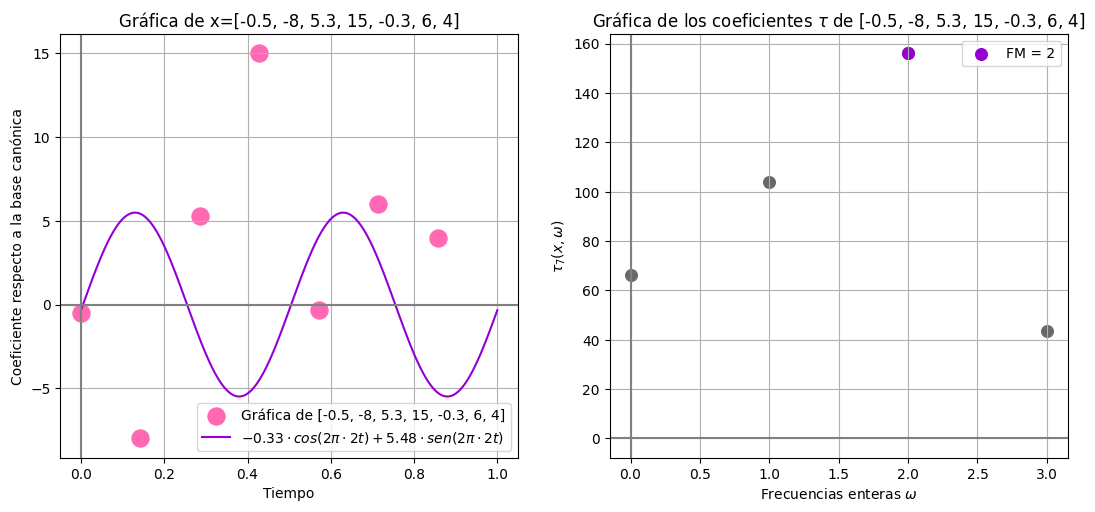
\includegraphics[scale = 0.45]{dft_espectro_1} 
\end{figure}	

Como se marca en el espectro con color morado, la frecuencia
asociada al coeficiente $\tau$ más alto es $\omega =2$; a la
izquierda, junto con la gráfica de la señal 
$x$, se dibuja el sinusoide (en versión continua)
de frecuencia $2$ que aparece en el análisis de
$x$ respecto a $\cali{F}_{7}$ dado en 
\eqref{eq: analisis x TDF}.
\final
\end{ejemplo}


\section{Metodología para realizar un análisis espectral que considere frecuencias arbitrarias}
\label{sec: metodologia para realizar un analisis espectral que considere frecuencias arbitrarias}

Ya podemos usar la base de Fourier real $\cali{F}_{n}$
definida en la proposición \ref{prop: base de fourier version real}
para hacer un estudio espectral de los PDL. \\

Puesto que, por la construcción de $\cali{F}_{n}$, 
hacer un análisis espectral de una señal $x \in \IR^{n}$
via su análisis respecto a la BON $\cali{F}_{n}$ nos lleva
a considerar sólo ciertas frecuencias enteras
(c.f. nota \ref{nota: frecuencias en las bases de fourier}),
queremos no sólo usar la TDF para realizar
nuestro estudio espectral, pues
no queremos restringirnos
al estudio de frecuencias enteras
(después de todo, según la hipótesis planteada en 
\ref{ref: hipotesis}, 
creemos que la frecuencia que mejor aproxima al PDL
$\cali{L}^{n,k}$ es $\frac{k}{2}$, y este último número no siempre
es un entero), sino que nos gustaría
\begin{enumerate}
	\item poder elegir una frecuencia $\omega \geq 0$ respecto
a la cual comparar a la señal y,
	\item una vez fijada una frecuencia, buscar el desfase $\phi \in [0,1]$
	que mejor ajuste la gráfica de $x$.
\end{enumerate}

\begin{figure}[H]
	\sidecaption{
	Aquí se grafica una misma señal $x \in \IR^{16}$ y se 
	compara con dos sinusoides de frecuencia $3.6$, una con 
	desfase (normalizado) 0.8 y otra con 0.32. Observe que
	la primera parece ajustar mucho mejor la gráfica de $x$.
	\label{fig: ejemplo desfase}
	}
	\centering
	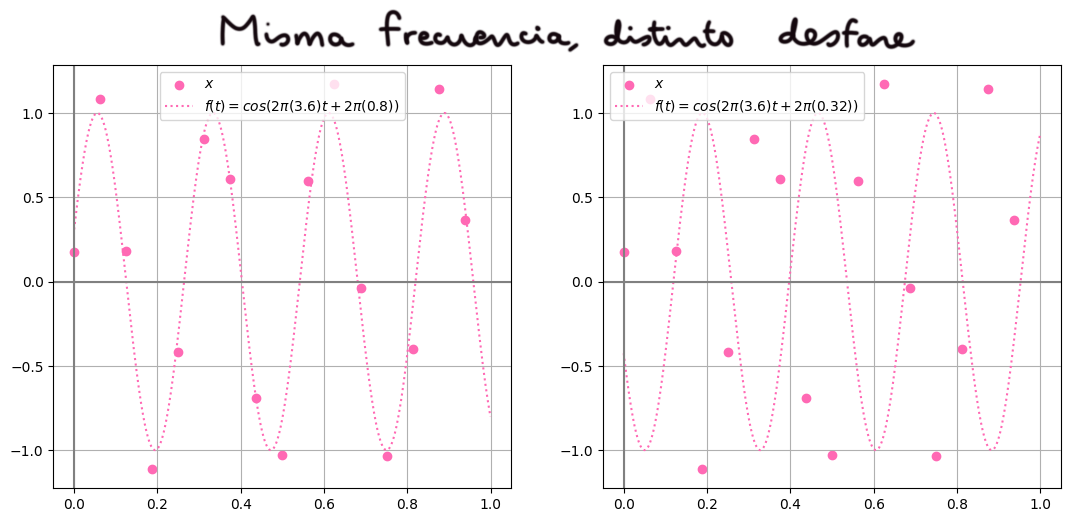
\includegraphics[scale=0.45]{desfase_ejemplo} 
\end{figure}	


Vamos a seguir
una linea de razonamiento totalmente análoga a la empleada 
en el ejemplo \ref{subs: ejm 3}, pues aquí también abordamos el problema
definiendo subconjuntos (de hecho, subespacios)
de $\IR^{n}$ que consten de elementos que cumplan
determinada propiedad (en el caso del ejemplo \ref{subs: ejm 3}, la propiedad
era ser elemento de determinado espacio 
de polinomios discretos $W_{n,k}$, mientras que 
en esta sección la propiedad de nuestro interés es ``ser la discretización
de un sinusoide de frecuencia $\omega$'') y usando el coseno del ángulo que
una señal $x$ forma con dichos subconjuntos para dar una medida de qué tanto
tiene $x$ la propiedad considerada.


\subsection{Espacios monofrecuenciales}

\begin{notacion}
Para simplificar la notación, denotamos por $I_{n}$ al intervalo
$\{ \frac{m}{n}  : 0 \leq m \leq n-1 \}$.
\end{notacion}

Digamos qué es lo que 
entendemos por ``señal de frecuencia pura $\omega$''.

\begin{defi}
Sean $n \in \IN$,  $\omega>0$, $\phi \in [0,1[$.  
A toda señal $n-$dimensional  
de la forma

\begin{equation}
A \left(
cos \left(  2 \pi \omega t + 2 \pi \phi
\right)
\right)_{t \in I_{n}}
\end{equation}

\noindent
con $A \in \IR$, se le llamará
\textbf{señal $n-$dimensional de frecuencia
pura $\omega$}. En este contexto,
a $\phi$ se le llama el \textbf{desfase normalizado}
de la señal, y a $A$ la \textbf{amplitud}.
\end{defi}

Note que los vectores
$c_{n, \omega}$ y $s_{n, \omega}$
definidos en la proposición
\ref{prop: base de fourier version real} son
señales $n-$dimensionales de frecuencia pura $\omega$.

\begin{nota}
Observe que toda señal de la forma
\begin{equation*}
A \left(
sin \left(  2 \pi \omega t + 2 \pi \phi
\right)
\right)_{t \in I_{n}},
\end{equation*}
con $A \in \IR$, también es una señal $n-$dimensional
de frecuencia pura $\omega$, pues, como 
\[
sen(x) = - cos (x+ \pi/2) \hspace{0.2cm}
\textit{para toda } x \in \IR,
\]
entonces
\begin{equation*}
A \left(
sin \left(  2 \pi \omega t + 2 \pi \phi
\right)
\right)_{t \in I_{n}} =
-A \left(
cos \left(  2 \pi \omega t + 2 \pi \phi^{'}
\right)
\right)_{t \in I_{n}},
\end{equation*}
donde $\phi^{'}= \phi + 1/4$.
\end{nota}


\begin{figure}[H]
	\sidecaption{
	Se grafica a la función 
	$f(t) = cos(2 \pi \cdot \frac{5}{2} t + 2 \pi \cdot 0.3)$;
	muestreando este sinusoide de forma uniforme con $n$
	puntos en el 
	intervalo [0,1] obtenemos una señal $n-$dimensional
	de frecuencia pura
	$\omega = \frac{5}{2}$. En la figura, $n=20$.
	\label{fig: desfasee ejemplo grafico}
	}
	\centering
	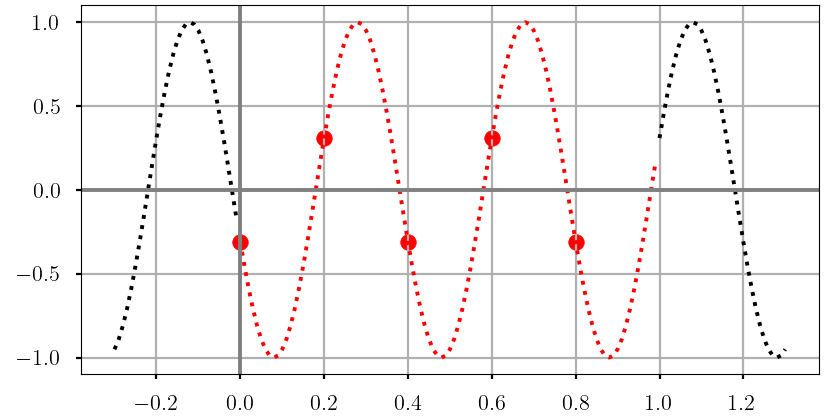
\includegraphics[scale= 0.55]{muestreo_coseno} 
\end{figure}	

\begin{prop}
\label{prop: para que frecuencias omega vector seno es cero}
	Sean $n \geq 2$, $\omega \geq 0$.
	\begin{itemize}
		\item El vector 
		\begin{equation}
		\label{eq: coseno omega}
		\tilde{c}_{n, \omega} = \left(cos(2 \pi \omega m/n) \right)_{m=0}^{n-1} \in \IR^{n}
		\end{equation}
		no es cero, y 
		\item el vector 
		\begin{equation}
		\label{eq: seno omega}
		\tilde{s}_{n, \omega} = \left(sen(2 \pi \omega m/n) \right)_{m=0}^{n-1} \in \IR^{n}
		\end{equation}
		es cero si y sólo si $\omega \in \frac{n}{2} \IZ$.
	\end{itemize}
\end{prop}
\noindent
\textbf{Demostración.}
El primer punto es fácil de probar, pues la primera entrada del
vector \eqref{eq: coseno omega} es 
$cos(0)=1$.

Supogamos ahora que $\omega>0$ es tal que \eqref{eq: seno omega}
es el vector cero, o sea, que
para toda $0 \leq m \leq n-1$, se tiene que 
$sen(2 \pi \omega m/n)=0$. En particular, ocurre
$sen(2 \pi \omega /n)=0$; esto implica la igualdad 
$2 \pi \omega /n = \pi K$ para algún entero $K$. Despejando
a $\omega$ de la ecuación tenemos que 
$\omega = \frac{n}{2}K \in \frac{n}{2} \IZ$. Recíprocamente,
todo $\omega$ de la forma 
$\frac{n}{2}K$, con $K \in \IZ$ hace que el vector 
\eqref{eq: seno omega} sea cero, pues, para toda $0 \leq m \leq n-1$,
$sen\left(2 \pi \frac{n}{2}K \frac{m}{n}\right)=
sen((Km)\pi)=0$.
\QEDB
\vspace{0.2cm}

Nos interesará considerar al subespacio
de $\IR^{n}$ generado por las señales
de frecuencia $\omega$ $\tilde{c}_{n, \omega}$
y $\tilde{s}_{n, \omega}$, o sea, a 

\begin{equation}
\label{eq: espacio Pnw}
P_{n, \omega} := span(\tilde{c}_{n, \omega}, \tilde{s}_{n, \omega}).
\end{equation} 
caracterizamos a los elementos de 
espacios de la forma
$P_{n, \omega}$ a continuación.

\begin{teo}
\label{prop: Pw consta de las señales de frecuencia omega}
Sean $n \in \IN$, $\omega \geq 0$ 
con 
$\omega \not\in \frac{n}{2} \IZ$.
El espacio $P_{n, \omega}$ definido en \eqref{eq: espacio Pnw} consta exactamente
de las señales $n$ dimensionales de frecuencia $\omega$.
\end{teo}

\noindent
\textbf{Demostración.}

Sea $\phi \in [0,1]$ un desfase cualquiera y $A \in \IR$
una amplitud cualquiera; por la regla
del coseno de la suma de dos ángulos, tenemos que
\[
A(cos (2 \pi \omega t + 2 \pi \phi))_{t \in I_{n}}
= Aa  (cos(2 \pi \omega t))_{t \in I_{n}} +
Ab  (sen(2 \pi \omega t))_{t \in I_{n}} \in P_{n, \omega} 
\]
donde
\[
a := cos (2 \pi \phi) \hspace{0.2cm} \text{y}
\hspace{0.2cm} b := sin (2 \pi  \phi).
\]


Recíprocamente, si $a, b \in \IR$ son escalares cualesquiera, 
el elemento genérico
$x=  a \left( cos \left(2 \pi \omega t \right) \right)_{t \in I_{n}} +
b ( sen (2 \pi \omega t ))_{t \in I_{n}} $ de $P_{n,w}$ puede
expresarse como sigue:

\begin{equation}
\label{eq1: 28Mar23}
x = \sqrt{a^{2}+b^{2}} \left(
A  \left( cos \left(2 \pi \omega t \right) \right)_{t \in I_{n}} +
B  \left( sin \left(2 \pi \omega t \right) \right)_{t \in I_{n}}
\right),
\end{equation}

\noindent
donde
\[
A := \frac{a}{\sqrt{a^{2}+b^{2}}} \hspace{0.2cm} \text{y} \hspace{0.2cm}
B := \frac{b}{\sqrt{a^{2}+b^{2}}}.
\]
Como $A^{2}+ B^{2}=1$, existe $\phi \in [0,1]$ tal que
\begin{equation}
\label{eq0: 28Mar23}
A = cos (2 \pi \phi) \hspace{0.2cm} \text{y}  \hspace{0.2cm}
B = sin (2 \pi \phi);
\end{equation}
sustituyendo \eqref{eq0: 28Mar23} en \eqref{eq1: 28Mar23}, llegamos
a que

\begin{align*}
x = &  \sqrt{a^{2}+b^{2}} (
cos(2 \pi \phi) \cdot (cos (2 \pi \omega t))_{t \in I_{n}} + 
sin(2 \pi \phi) \cdot (sin (2 \pi \omega t))_{t \in I_{n}} 
) \\
= & \sqrt{a^{2}+b^{2}} (
cos(2 \pi \phi) \cdot cos (2 \pi \omega t) +
sin(2 \pi \phi) \cdot sin (2 \pi \omega t) 
)_{t \in I_{n}}  \\
= &  \sqrt{a^{2}+b^{2}} (
cos (2 \pi \omega t - 2 \pi \phi)
)_{t \in I_{n}}.
\end{align*}

\QEDB
\vspace{0.2cm}

\begin{defi}
Si $n \geq 2$ y $\omega>0$, entonces
al subespacio $P_{n,\omega}$ 
de $\IR^{n}$
definido en \eqref{eq: espacio Pnw} 
le llamaremos el \textbf{espacio monofrecuencial
$n$ dimensional} de frecuencia $\omega$.
\end{defi}

\begin{obs}
\label{obs aa: f y g son l.i. y de norma uno}
Sean $n \geq 2$ entero, $\omega \geq 0$ con $\omega \not\in \frac{n}{2} \IZ$.
Los vectores \eqref{eq: coseno omega} y \eqref{eq: seno omega}
de $\IR^{n}$ son linealmente independientes.
\end{obs}
\noindent
\textbf{Demostración.}
Sólo note que 
la primera entrada de \eqref{eq: coseno omega} es $1$, mientras que  
la primera entrada de $\tilde{s}_{n, \omega}$ es cero pero no
todas sus entradas lo son (c.f. proposición 
\ref{prop: para que frecuencias omega vector seno es cero}). 
\QEDB
\vspace{0.2cm}


Según la observación 
\ref{obs aa: f y g son l.i. y de norma uno}, si $\omega \not\in \frac{n}{2} \IZ$,
el espacio $P_{n,\omega}$ que generan los vectores 
\eqref{eq: coseno omega} y \eqref{eq: seno omega}

\begin{align}
\label{eq6: 23Ap}
P_{n,\omega}:= & span( \tilde{c}_{n, \omega}, 
\tilde{s}_{n, \omega}) \notag  \\  
= &
\{ a \left( cos \left(2 \pi \omega t \right) \right)_{t \in I_{n}} +
b ( sen (2 \pi \omega t ))_{t \in I_{n}} : 
\hspace{0.2cm} a, b \in \IR \},
\hspace{0.1cm} \omega \not\in \frac{n}{2} \IZ
\end{align}

\noindent
es un plano (i.e. un subespacio de dimensión $2$) de $\IR^{n}$
que además, según el teorema 
\ref{prop: Pw consta de las señales de frecuencia omega},
consta exactamente de las señales
de dimensión $n$ y frecuencia (pura) $\omega$. \\

Si $\omega \in \frac{n}{2} \IZ$, entonces, según 
la proposición 
\ref{prop: para que frecuencias omega vector seno es cero}, el vector
$\tilde{s}_{n, \omega}$ es el vector cero y 
$\tilde{c}_{n, \omega}$ no, luego, el espacio
\begin{align}
\label{eq0: 23Ap}
P_{n,\omega}:= & span(c_{n, \omega}, s_{n, \omega}) \notag  \\  
= &
\{ a \left( cos \left(2 \pi \omega t \right) \right)_{t \in I_{n}} : 
\hspace{0.2cm} a \in \IR \},
\hspace{0.1cm} \omega \in \frac{n}{2} \IZ
\end{align}
es una recta (i.e. un subespacio de dimensión $1$)
de $\IR^{n}$.

\begin{nota}
Sean $n \geq 2$, $\omega \in \frac{n}{2} \IZ$ 
una frecuencia
mayor o igual a cero; digamos que 
$\omega = \frac{n}{2}K$. Entonces, 
según la proposición 
\ref{prop: para que frecuencias omega vector seno es cero},
$s_{n, \omega} =0$ y
\[
\tilde{c}_{n, \omega} = \left(cos\left( 2 \pi \frac{n}{2}K \frac{m}{n}\right)
\right)_{m=0}^{n-1}
= (cos(mK \pi))_{m = 0}^{n-1} = ((-1)^{mK})_{m=0}^{n-1},
\]
luego, 
fijada una dimensión $n$, sólo hay dos espacios
$P_{n, \omega}$ cuando 
$\omega \in \frac{n}{2} \IZ$,
a saber,
\[
\{ (a)_{m=0}^{n-1} : \hspace{0.2cm} a \in \IR \} \subseteq \IR^{n}
\]
y
\[
\{ ((-1)^{m}a)_{m=0}^{n-1} : \hspace{0.2cm} a \in \IR \} \subseteq \IR^{n}.
\]

\end{nota}

\section{Caso particular en el que el subespacio en cuestión es un plano}
\label{ap: Caso particular en el que el subespacio en cuestión es un plano}

\TODO{Cambiar título e intro porque moví esto.}
Necesitaremos concentrarnos en el caso
particular en el que el subespacio cerrado $W$ es 
un plano,\sidenote{O sea, un subespacio
de dimensión $2$.} por lo que a continuación elaboramos un poco más
la teoría de la sección 
\ref{angulo entre elementos de un espacio con producto punto}
para este caso particular.

La situación es la siguiente: $V$ es un $\IR-$espacio
de Hilbert, $u$ y $v$ son elementos de $V$,
unitarios y linealmente
independientes entre sí. El espacio que ellos generan
es pues un plano, digamos,


\[
P := span \{ u, v \}.
\]

Dado $x \in V$,
el coseno del ángulo entre $x$ y $W$ es,
según la proposición
\ref{prop: algunos hechos sobre el angulo entre un vector y un subespacio},

\begin{equation}
\label{eq0: 19Marzo}
cos \left( \measuredangle (x, P) \right) = 
\frac{|| \Pi_{P}(x) ||}{||x||};
\end{equation}
para lograr expresar el lado derecho de la igualdad en términos
sólo de $u$, $v$ y $x$ (que son los elementos básicos de
nuestra discusión), conviene primero obtener, a partir 
de estos elementos, una base
ortonormal del espacio $P$.


\begin{obs}
Si $u, v \in V$ son unitarios y linealmente independientes, y $P$
es el plano que generan, entonces
$\{ u, z \}$, donde

\begin{equation}
\label{eq2: 19Marzo}
z:= \frac{v- \langle u, v \rangle u}{||v- \langle u, v \rangle u||}
\end{equation}
es una BON de $P$
\end{obs}
\noindent
\textbf{Demostración.}
Basta aplicar el teorema de Gram-Schmidt 
\ref{Teo:Gram-Schmidt}.
\QEDB
\vspace{0.2cm}

Teniendo una BON de $P$, según el 
corolario 
\ref{cor: proyeccion en terminos de BON}, se tiene la siguiente
expresión para la proyección de $x$ en $P$;

\begin{equation}
\label{eq1: 19Marzo}
\Pi_{P}(x)= \langle x, u \rangle u + \langle x, z \rangle z;
\end{equation}

\noindent
puesto que, según la definición \eqref{eq2: 19Marzo} de 
$z$ este vector es función de $u$ y $v$, fácilmente se
puede derivar, a partir de \eqref{eq1: 19Marzo},
una expresión de $\Pi_{P}(x)$ en función sólo
de $x$, $u$ y $v$. Se plasman las fórmulas 
concretas a continuación.
	\begin{prop}
	\label{prop: formulas 20Marzo}
	Sean $V$ un espacio de Hilbert, $x \in V$,
	$u,v \in V$ linealmente independientes
	y unitarios. Si $P$ es el plano
	que generan $u$ y $v$, entonces,

		\begin{equation}
		\label{eq0: 24ap}
		\Pi_{P}(x)= \frac{\langle x, u \rangle -\langle u, v \rangle \langle x, v \rangle }{1-\langle u, v \rangle^{2}} u + \frac{\langle x, v \rangle -\langle u, v \rangle \langle x, u \rangle }{1-\langle u, v \rangle^{2}} v
		\end{equation}
	y 
		\begin{equation}
		\label{eq3: 19Marzo}
		  || \Pi_{P}(x) ||^{2}=
		  \frac{\langle x, u \rangle^{2} +  \langle x, v \rangle^{2}	
	       -2  \langle x, u \rangle \langle x, v \rangle \langle u, v \rangle	}{1- \langle u, v 		\rangle^{2}}.
		\end{equation}
 
	\end{prop}

\noindent
\textbf{Demostración.}
La demostración consiste de simples manipulaciones aritméticas.
Según \eqref{eq1: 19Marzo},
\begin{align*}
\Pi_{P}(x) = & \langle x, u \rangle u + \langle x, z \rangle z \\
 = & \langle x, u \rangle u
 + \frac{\langle x, v \rangle - \langle u, v \rangle \langle x, u \rangle}{|| v -\langle u,v \rangle u ||^{2}}
(v - \langle u,v \rangle u);\\
\end{align*}

\noindent
puesto que $u$ y $v$ son unitarios, 
tenemos que
\begin{align}
\label{eq3: 23ap}
|| v -\langle u,v \rangle u ||^{2} = & 
\langle v,v \rangle^{2} -2
\langle u,v \rangle^{2} +\langle u,v \rangle^{2}\langle u,u \rangle \notag  \\
= & 1 -\langle u,v \rangle^{2}; 
\end{align}
sustituyendo \eqref{eq3: 23ap} en la última expresión para 
$\Pi_{P}(x)$ llegamos a \eqref{eq3: 19Marzo}. \\

Finalmente, 
\begin{align*}
|| \Pi_{P}(x) ||^{2} = & 
\langle x,u \rangle^{2} + \langle x,z \rangle^{2} \\
= & \langle x,u \rangle^{2} + 
\left(
\frac{\langle x,v \rangle - \langle u,v \rangle
\langle x,u \rangle}{||v -\langle u,v \rangle u ||}
\right)^{2};\\
\end{align*}

\noindent
sustituyendo \eqref{eq3: 23ap} en esta última expresión
llegamos a \eqref{eq4: 19Marzo}.

\QEDB
\vspace{0.2cm}

Usando las expresiones
\eqref{eq: coseno a subespacio}
y \eqref{eq3: 19Marzo} es fácil establecer
la siguiente proposición.

\begin{prop}
Sean $V$ un espacio de Hilbert, $x \in V$,
	$u,v \in V$ linealmente independientes
	y unitarios. Si $P$ es el plano
	que generan $u$ y $v$, entonces,
	
	
\begin{equation}
\label{eq: coseno a plano}
cos (\measuredangle (x, P)) = 
\sqrt{
\frac{\langle x, u \rangle^{2} +  \langle x, v \rangle^{2}	
	       -2  \langle x, u \rangle \langle x, v \rangle \langle u, v \rangle	}{
	       ||x||^{2} \cdot 
	       (1- \langle u, v 	\rangle^{2})  }}.
\end{equation}
\end{prop}

\subsection{Estudio espectral basado en ángulos a espacios monofrecuenciales}

Definidos los espacios monofrecuenciales
$P_{n, \omega} \subseteq \IR^{n}$ 
(c.f. \eqref{eq: espacio Pnw})
y caracterizados sus elementos como las señales
$n-$dimensionales de frecuencia pura $\omega$,
parece razonable
medir la cercanía de una señal $n-$dimensional $x \in \IR^{n}$
a tener frecuencia $\omega$
con el ángulo que $x$ forma con el subespacio $P_{n, \omega}$,
cuyo coseno, según la proposición
\ref{prop: algunos hechos sobre el angulo entre un vector y un subespacio}
es
\begin{equation}
\label{eq0: 20Mar}
cos \left( \measuredangle (x, P_{n, \omega}) \right) = 
\frac{|| \Pi_{P_{n, \omega}}(x) ||}{||x||}
\in [0,1].
\end{equation}


\begin{figure}[H]
	\sidecaption{
	Según la relación \eqref{eq0: 20Mar}, 
	si $\frac{||\Pi_{P_{\omega}}(x)||}{||x||}$ es cercano 
	a uno (resp. a cero), entonces $x$ es muy parecido a una señal de frecuencia $\omega$
	(resp. se aleja de ser una señal de frecuencia $\omega$).
	\label{fig: 20Mar23_1}
	}
	\centering
	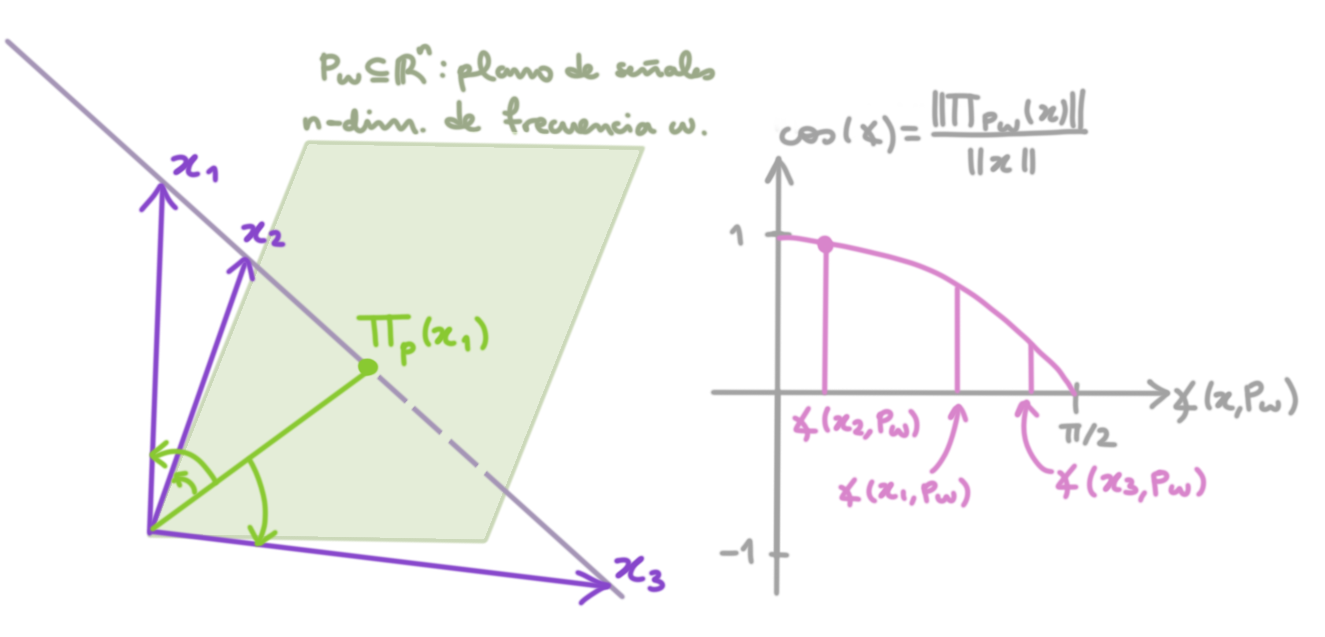
\includegraphics[scale= 1]{20Mar23_1} 
\end{figure}	

Si $x$ es unitaria,
tenemos la relación simplificada 

\begin{equation}
\label{eq1: 20Mar}
cos \left( \measuredangle (x, W) \right) = || \Pi_{W}(x) || 
\hspace{0.5cm} (x \hspace{0.1cm} \text{unitario).}
\end{equation}


\textbf{Usaremos pues, para dar una medida de qué tanto
reacciona una señal $x \in \IR^{n}$ a una frecuencia
$\omega >0$
el número 
\[\frac{||\Pi_{P_{n, \omega}}(x)||}{||x||} \in [0,1].\]} \\

\begin{defi}
\label{def: final de sigmas}
Sean $n \geq 2$, $\omega \geq 0$. 
Definimos la función $\sigma_{n}(\cdot, \omega)$ para todo 
elemento de $\IR^{n} - \{ 0\}$
como sigue;
\begin{equation}
\label{eq: def sigmas}
	\forall x \in \IR^{n}-\{ 0\}: \hspace{0.2cm}
	\sigma_{n}(x, \omega) =
	cos \left( \measuredangle (x, P_{n, \omega}) \right) = 
	\frac{||\Pi_{P_{n, \omega}}(x)||}{||x||} .
\end{equation}
\end{defi}

\begin{nota}
\label{nota: significado de los sigma en AE}
Fijada una frecuencia $\omega$, 
\begin{itemize}
\item si $\sigma_{n, \omega}(x)$ es ``cercano'' a cero, $\omega$ no
es una frecuencia con la que es razonable aproximar a $x$ (pues $x$ será
cercano a ser ortogonal a toda señal de dimensión $n$ y frecuencia 
$\omega$),  mientras que

\item si $\sigma_{n, \omega}(x)$ es ``cercano'' a uno, también es muy cercano
(hablando en términos de distancia euclídea) a su proyección al espacio
$P_{n, \omega}$, luego $x$ es muy parecido a tener frecuencia $\omega$.
\end{itemize}
\end{nota}



Para poder usar las fórmulas
derivadas en la subsección 
\ref{ap: Caso particular en el que el subespacio en cuestión es un plano},
debemos de dar una BON del espacio $P_{n, \omega}$.

\begin{prop}
\label{prop: aaa}
Sean $n \in \IN$, $\omega>0$. Sean los vectores 
$\tilde{c}_{n, \omega}, 
\tilde{s}_{n ,\omega} \in \IR^{n}$ 
como se definieron en 
\eqref{eq: coseno omega} y \eqref{eq: seno omega}, 
respectivamente.
\begin{itemize}
	\item Si $\omega \not\in \frac{n}{2} \IZ$, entonces 
	$\{ c_{n, \omega}, s_{n, \omega} \}$, donde

	\begin{equation}
	\label{eq5: 19Marzo}
	c_{n, \omega}=\xi_{n, \omega} \tilde{c}_{n, \omega}
	\in \IR^{n}
	\end{equation}
y 

	\begin{equation}
	\label{eq6: 19Marzo}
	s_{n, \omega}= \eta_{n, \omega} \tilde{s}_{n, \omega}
	\in \IR^{n},
	\end{equation}
con 
\begin{equation}
\label{eq7: 19Marzo}
	\xi_{n, \omega}= 
	\sqrt{2} \cdot \left( n + \frac{sen(2 \pi \omega)
	cos(2 \pi \omega \left(\frac{n-1}{n} \right))}{sen \left(2 \pi 
	\frac{\omega}{n} \right)} \right)^{-\frac{1}{2}} 
\end{equation}
y

	\begin{equation}
	\label{eq8: 19Marzo}
	\eta_{n, \omega}= \sqrt{2} \cdot \left( n - \frac{sen(2 \pi \omega)
	cos(2 \pi \omega \left(\frac{n-1}{n} \right))}{sen \left(2 \pi 
	\frac{\omega}{n} \right)} \right)^{-\frac{1}{2}}
	\end{equation}

\noindent
es una base normalizada del subespacio $P_{n, \omega} \leq \IR^{n}$
definido en \eqref{eq6: 23Ap}, y,
\item si $\omega \in \frac{n}{2} \IZ$, entonces 
$\{ c_{n, \omega} \}$, con
\begin{equation}
\label{ec: 4: 23ap}
	c_{n, \omega} := \frac{1}{\sqrt{n}} \tilde{c}_{n, \omega}
\end{equation}
es una base normalizada 
del subespacio $P_{n, \omega} \leq \IR^{n}$
definido en \eqref{eq0: 23Ap}.
\end{itemize}
\end{prop}
\noindent
\textbf{Demostración.}
En efecto, por definición del espacio
$P_{n, \omega}$, $\{ \tilde{c}_{n, \omega}, 
\tilde{s}_{n, \omega} \}$
es una base de este cuando
$\omega \not\in \frac{n}{2}\IZ$, y
$\{ \tilde{c}_{n, \omega}\}$ es base si 
$\omega \in \frac{n}{2}\IZ$,
luego, en ambos casos el conjunto propuesto en efecto
es una base de $P_{n, \omega}$.
En el segundo caso, puesto que
$c_{n, \omega}$ será un vector cuyas entradas serán $1$, o $-1$,
en efecto es un vector unitario. 
En el primer caso, se han calculado las constantes 
$\xi_{n, \omega}$ y $\eta_{n, \omega}$
dadas en 
\eqref{eq7: 19Marzo} y \eqref{eq8: 19Marzo}
para que $c_{n, \omega}$ y $s_{n, \omega}$
tengan normal uno; puesto que los cálculos son muy
similares a los realizados en la demostración de la proposición
\ref{prop: producto punto entre f y g}, los omitimos.
\QEDB
\vspace{0.2cm}


\begin{nota}
\label{nota: notacion cnw, snw}
Observe que las notaciones 
``$c_{n, \omega}$'' y ``$s_{n, \omega}$'' ya las
habíamos empleado antes en la proposición 
\ref{prop: base de fourier version real} cuando se definía
la base ortonormal en función de la cual se calcula la TDF; no hay problema
en usar esta notación aquí también, pues para los valores 
$\omega \in Dom_{TDF, n}$, los vectores
$c_{n, \omega}$ y $s_{n, \omega}$ definidos en 
la proposición \ref{prop: base de fourier version real}
coinciden con los que acabamos de defininir en la proposición 
\ref{prop: aaa}.
\end{nota}

Conviene también establecer una fórmula para
el producto punto entre 
los vectores $c_{n, \omega}$ y $s_{n, \omega}$
definidos en la proposición \ref{prop: aaa}
cuando $\omega \not\in \frac{n}{2} \IZ$.
Hacemos esto a continuación.

\begin{prop}
\label{prop: producto punto entre f y g}
Fijados $n \geq 2$ y $\omega \geq 0$ con 
$\omega \not\in \frac{n}{2}\IZ$, 
el producto punto entre 
los vectores
$c_{n, \omega}$ y $s_{n, \omega}$, definidos 
\eqref{eq5: 19Marzo} y \eqref{eq6: 19Marzo}
respectivamente, es

\begin{equation}
\label{eq9: 19Marzo}
\langle c_{n, \omega} , s_{n, \omega} \rangle =
\frac{\xi_{n, w} \eta_{n, \omega}}{2} \cdot 
\frac{sen(2 \pi \omega)
sen(2 \pi \omega \left( 1- \frac{1}{n} \right))}{sen \left(2 \pi 
\frac{\omega}{n} \right)}
\end{equation}

\end{prop}
\noindent
\textbf{Demostración.}
Aquí usaremos las siguientes tres igualdades:

\begin{equation}
\label{eq10: 19Marzo}
\forall \alpha \in \IR: \hspace{0.2cm}
sen(2 \alpha) = 2 sen(\alpha) cos(\alpha),
\end{equation}



\begin{equation}
\label{eq11: 19Marzo}
\forall z\in \IR: \hspace{0.2cm}
sen(z)= \frac{e^{iz}-e^{-iz}}{2i},
\end{equation}



\begin{equation}
\label{eq12: 19Marzo}
\forall a \in \IR-\{ 1 \}: \hspace{0.2cm}
\suma{m=0}{n-1}{a^{r}}= \frac{1-a^{n}}{1-a}.
\end{equation}

\noindent
Tenemos que

\begin{align*}
\langle c_{n,\omega} , s_{n, \omega} \rangle = &
\xi_{n, \omega} \eta_{n, \omega} \left\langle 
\left( cos \left( 2 \pi \omega \frac{m }{n} \right) \right)_{0 \leq m \leq N-1} ,  
\left( sen \left( 2 \pi \omega \frac{m }{n}\right) \right)_{0 \leq m \leq N-1} \right\rangle \\
= & \xi_{n, \omega} \eta_{n, \omega} \suma{m=0}{n-1}{
cos \left(2 \pi \omega \frac{m}{n}\right) sen\left( 2 \pi \omega \frac{m}{n}\right)} \\
= & \frac{\xi_{n, \omega} \eta_{n, \omega}}{2}
\suma{m=0}{n-1}{
\left( sen\left( 4 \pi \omega \frac{m}{n}\right) \right)} \\
= & \frac{\xi_{n, \omega} \eta_{n, \omega}}{4i} \suma{m=0}{n-1}{
\left( e^{4 \pi \omega i m/n} - 
e^{-4 \pi \omega i m/n} \right) } \\
= & \frac{\xi_{n, \omega} \eta_{n, \omega}}{4i} 
\left(
\frac{1-e^{4 \pi \omega i }}{1-e^{4 \pi \omega i /N}} - 
\frac{1-e^{-4 \pi \omega i }}{1-e^{-4 \pi \omega i /N}} 
\right) \\
= & \frac{\xi_{n, \omega} \eta_{n, \omega}}{4i} 
\left(
\frac{e^{2 \pi \omega i }}{e^{2 \pi \omega i/n }}
\frac{e^{-2 \pi \omega i }-e^{2 \pi \omega i }}{e^{-2 \pi \omega i/n }-e^{2 \pi \omega i /N}} - 
\frac{e^{-2 \pi \omega i }}{e^{-2 \pi \omega i/n }}
\frac{e^{2 \pi \omega i }-e^{-2 \pi \omega i }}{e^{2 \pi \omega i/n }-e^{2 \pi \omega i /N}} 
\right) \\
= & 
\frac{\xi_{n, \omega} \eta_{n, \omega}}{4i} 
\left(
e^{2 \pi \omega i \left( 1-1/n \right)}
\frac{sen(2 \pi \omega)}{sen(2 \pi \omega /n)} - 
e^{-2 \pi \omega i \left( 1-1/n \right)}
\frac{sen(2 \pi \omega)}{sen(2 \pi \omega /n)}
\right) 
\\
= & 
\frac{\xi_{n, \omega} \eta_{n, \omega}}{4i} 
\frac{sen(2 \pi \omega)}{sen(2 \pi \omega /n)}
\left(
e^{2 \pi \omega i \left( 1-1/n \right)} - e^{-2 \pi \omega i \left( 1-1/n \right)}
\right) \\
= &
\frac{\xi_{n, \omega} \eta_{n, \omega}}{4i} 
\frac{sen(2 \pi \omega)}{sen(2 \pi \omega /n)}
\left(
2i \cdot  sen \left( 2 \pi \omega  \left( 1- \frac{1}{n} \right) \right)
\right)\\
= & 
\frac{\xi_{n, \omega} \eta_{n, \omega}}{2} 
\frac{sen(2 \pi \omega)}{sen(2 \pi \omega /n)}
sen \left( 2 \pi \omega  \left( 1- \frac{1}{n} \right) \right). \\
\end{align*}
\QEDB
\vspace{0.2cm}



\begin{prop}
\label{prp: ammm}
Sean $n \geq 2$, $\omega \geq 0$. 
Sea $\sigma_{n}(\cdot,\omega): \IR^{n} \longrightarrow [0,1]$
la función definida en \ref{def: final de sigmas}.
Para todo $x \in \IR^{n}-\{ 0 \}$
se tiene que
\begin{itemize}
	\item Si $\omega \not\in \frac{n}{2} \IZ$, entonces
	\begin{equation}
	\label{eq: pi ommm 1}
	 \Pi_{P_{n, \omega}}(x) = 
\frac{
\langle x, c_{n, \omega} \rangle - \langle c_{n, \omega}, s_{n, \omega} \rangle 
\langle x, s_{n, \omega} \rangle
}
{1-|\langle c_{n, \omega}, s_{n, \omega} \rangle |^{2}  }
c_{n, \omega} +
\frac{
\langle x, s_{n, \omega} \rangle - \langle c_{n, \omega}, s_{n, \omega} \rangle 
\langle x, c_{n, \omega} \rangle
}
{1-|\langle c_{n, \omega}, s_{n, \omega} \rangle |^{2}  }
s_{n, \omega}
	\end{equation}
	y 
	\begin{equation}
	\label{eq: coef sigma caso 1}
	\sigma_{n}(x, \omega) =
	\left(		  
		  \frac{\langle x, c_{n, \omega } \rangle^{2} +  \langle x, s_{n, \omega } \rangle^{2}	
	       -2  \langle x, c_{n, \omega } \rangle \langle x, s_{n, \omega } \rangle \langle c_{n, \omega }, s_{n, \omega } \rangle}{ || x ||^{2} \cdot
	       (1- \langle c_{n, \omega }, s_{n, \omega } \rangle^{2})}	  
\right) ^{1/2},
	\end{equation}
donde $c_{n, \omega}$ y $s_{n, \omega}$ son como en 
\eqref{eq5: 19Marzo} y \eqref{eq6: 19Marzo}, y

\item si $\omega \in \frac{n}{2} \IZ$, entonces 
\begin{equation}
\label{eq: pi ommm 2}
\Pi_{P_{n, \omega}}(x) = \langle x, c_{n, \omega} \rangle c_{n, \omega}
\end{equation}
y 
\begin{equation}
\label{eq: sfklmslsfl}
\sigma_{n}(x, \omega) = \frac{|\langle x, c_{n, \omega} \rangle |}{||x||},
\end{equation}
donde $c_{n, \omega}$ es como en \eqref{ec: 4: 23ap}.
\end{itemize}
\end{prop}



Ya tenemos todo lo necesario para dar una definición alternativa 
del espectro de una señal 
(c.f. definición
\ref{def: espectro DFT} para ver la definición de espectro
basada en la TDF).

\begin{comment}
\begin{nota}
Observe lo siguiente; fijadas una dimensión $n$
y una señal $x \in \IR^{n}$, si 
$\omega \in [0, \frac{n}{2}]$, entonces
\begin{equation}
\label{eq0: 1May}
\sigma_{n}(x, \omega) = \sigma_{n}(x, \omega + n/2).
\end{equation}

\noindent
En efecto, para toda $0 \leq m \leq n-1$,
por la regla del coseno de la suma de dos ángulos,
\[
cos\left(2 \pi \left( \omega + \frac{n}{2} \right) \frac{m}{n} \right)
= (-1)^{m} cos \left( 2 \pi \omega \frac{m}{n} \right)
\] 
y, similarmente, 
\[
sen \left(2 \pi \left( \omega + \frac{n}{2} \right) \frac{m}{n} \right)
= (-1)^{m} sen \left( 2 \pi \omega \frac{m}{n} \right),
\] 
luego, se tienen las igualdades \[
c_{n, \omega} =  2_{n, \omega + n/2}
\]
y \[
s_{n, \omega} = s_{n, \omega + n/2},
\] 
por lo tanto, 
\begin{align*}
P_{\omega + \frac{n}{1}} := & span(c_{n, \omega}, s_{n, \omega}) \\
= &  span(c_{n, \omega}, s_{n, \omega})
\end{align*}
\TODO{general al mismo P omega, por eso los sigmas son iguales.}
\end{nota}
\end{comment}

\section{Desfase de la proyección de una señal a espacios monofrecuenciales}


Fijada una dimensión $n$ y 
una frecuencia $\omega \geq 0$,
dado cualquier 
$x \in \IR^{n}-\{ 0 \}$
ya tenemos una fórmula para calcular la
proyección $\Pi_{P_{n, \omega}}(x)$ 
(c.f. proposición \ref{prp: ammm}).
Sin embargo, 
como
$\Pi_{P_{n, \omega}}(x) \in P_{n, \omega}$, 
según el teorema 
\ref{prop: Pw consta de las señales de frecuencia omega}, 
es posible expresar a la señal $\Pi_{P_{n, \omega}}(x)$
como el resultado de muestrear uniformemente con $n$ mediciones
a un sinusoide de frecuencia pura $\omega$. Lo que queremos hacer
en esta sección es dar explícitamente a los dos elementos que
faltan para determinar univocamente este sinusoide continuo,
a saber, el parámetro de amplitud $A \in \IR$ y el 
desfase normalizado $\phi \in [0,1[$. Buscamos entonces $A$
y $\phi$ tales que
\[
\Pi_{P_{n, \omega}}(x) = A (cos(2 \pi \omega t -  2 \pi \phi ))_{t \in I_{n}}.
\]
 
\marginnote{Buscamos pues la amplitud y el desfase de la señal
de frecuencia $\omega$ más cercana a $x$.}

Puesto que
$\Pi_{P_{n, \omega}}(x)$ (donde $P_{n, \omega}$ es como se definió en 
\eqref{eq: espacio Pnw}) 
es la señal de frecuencia $\omega$ que está a menor
distancia euclidea de $x$, podremos interpretar este
desfase $\phi$ como el desfase que mejor se ajusta a $x$
(c.f. figura \ref{fig: desfasee ejemplo grafico}). \\

Primero abordemos el caso en el que
$\omega \not\in \frac{n}{2} \IZ$. 

Como los vectores $c_{n, \omega}$ y $s_{n, \omega}$ 
definidos en \eqref{eq5: 19Marzo} y \eqref{eq6: 19Marzo}
son unitarios y linealmente independientes (c.f. proposición
\ref{prop: aaa}),
podemos usar la ecuación \eqref{eq0: 24ap}
para escribir a la proyección de $x$ en $P_{\omega}$ como sigue


\begin{equation}
\label{eq3: 20Marzo}
\Pi_{P_{\omega}}(x)= c (cos (2 \pi \omega t))_{t \in I_{n}} + d 
(sin (2 \pi \omega t))_{t \in I_{n}},
\end{equation}
donde

\begin{equation}
\label{eq4: 20Marzo}
c= \frac{
\langle x, c_{n, \omega} \rangle - \langle c_{n, \omega}, s_{n, \omega} \rangle
\langle x, s_{n, \omega} \rangle
}{1-\langle c_{n, \omega}, s_{n, \omega} \rangle^{2}} \xi_{n, \omega}
\end{equation}
y
\begin{equation}
\label{eq5: 20Marzo}
d= \frac{
\langle x, s_{n, \omega} \rangle - \langle c_{n, \omega}, s_{n, \omega} \rangle
\langle x, c_{n, \omega} \rangle
}{1-\langle c_{n, \omega}, s_{n, \omega} \rangle^{2}} \eta_{n, \omega}.
\end{equation}

\noindent 
Nos conviene más reescribir a \eqref{eq3: 20Marzo} como
\begin{equation}
\label{eq6: 20Marzo}
\Pi_{P_{n, \omega}}(x)= 
\sqrt{c^{2}+d^{2}}
\left[
C (cos (2 \pi \omega t))_{t \in I_{n}} +
D (sen (2 \pi \omega t))_{t \in I_{n}} 
\right],
\end{equation}

\noindent 
donde

\begin{equation}
\label{eq3: 28Marz23}
C:= \frac{c}{\sqrt{c^{2}+d^{2}}} \hspace{0.2cm} \text{y}
\hspace{0.2cm} D:= \frac{d}{\sqrt{c^{2}+d^{2}}},
\end{equation}
\noindent 
pues, como $C^{2} + D^{2}=1$, existe un único
$\phi \in [0,1[$ tal que
\begin{equation}
\label{eq7: 20Marzo}
C= cos(2 \pi \phi), \hspace{0.2cm} 
D= sin(2 \pi \phi).
\end{equation}

\noindent 
Sustituyendo \eqref{eq7: 20Marzo} en \eqref{eq6: 20Marzo},
llegamos a que

\begin{align*}
\Pi_{P_{n, \omega}}(x) = & 
\sqrt{c^{2}+d^{2}} \left[
cos(2 \pi \phi) \cdot (cos (2 \pi \omega t))_{t \in I_{n}} +
sin(2 \pi \phi) \cdot (sin (2 \pi \omega t))_{t \in I_{n}} 
\right] \\
= & 
\sqrt{c^{2}+d^{2}} 
(cos(2 \pi \phi) \cdot cos (2 \pi \omega t) +
sin(2 \pi \phi) \cdot sin (2 \pi \omega t) )_{t \in I_{n}} \\
= & 
\sqrt{c^{2}+d^{2}} 
(cos(2 \pi \omega t - 2 \pi \phi))_{t \in I_{n}}.
\end{align*}

\noindent
Además, de \eqref{eq7: 20Marzo} y \eqref{eq3: 28Marz23}
se deduce que
\begin{marginfigure}
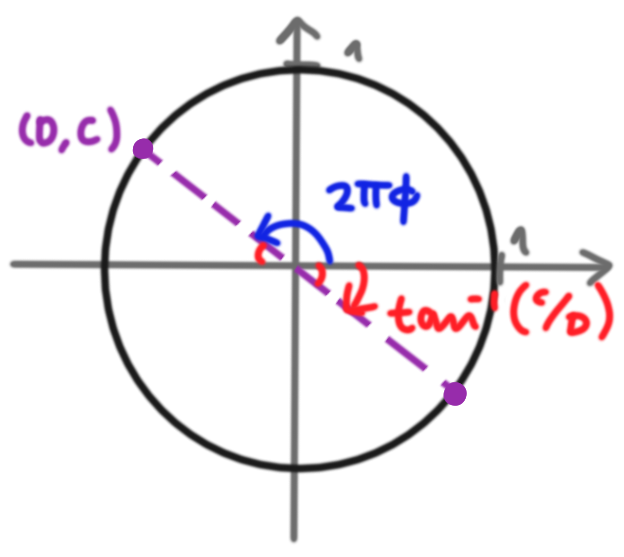
\includegraphics[scale= 0.8]{encontrado_desfase} 
\end{marginfigure}
\begin{equation}
\label{eq: desfase phi 1}
\phi =
\begin{cases}
\frac{tan^{-1}(d/c) }{2 \pi}  \hspace{0.4cm}    \text{   si }   d, c > 0,  \\
\frac{tan^{-1}(d/c) + \pi }{2 \pi} \hspace{0.2cm}  \text{si }  d, c < 0
\text{ o } d<0, c>0, \\
\frac{tan^{-1}(d/c) + 2\pi }{2 \pi} \hspace{0.2cm}  \text{si }  d>0,  c < 0. 
\end{cases}
\end{equation}


Hemos probado el siguiente
\begin{teo}
\label{teo: amelie1}
\textbf{(Amplitud y desfase de la proyección de $x \in \IR^{n}$ al
espacio monofrecuencial $P_{n, \omega}$)}
Sean $n \geq 2$ y $\omega > 0$ con $\omega \not\in \frac{n}{2}\IZ$.
Si $P_{n, \omega}$ es el subespacio de $\IR^{n}$ definido como 
en \eqref{eq6: 23Ap}, entonces, para todo 
$x \in \IR^{n}$ no cero, se tiene que
\begin{equation}
\label{ec: desfase explicito 1}
\Pi_{P_{n, \omega}} (x) = A \cdot (
cos (2 \pi \omega t - 2 \pi \phi)
)_{t \in I_{n}} \in \IR^{n},
\end{equation}

\noindent
donde la amplitud $A$ es
\[
\sqrt{c^{2}+d^{2}},
\]
$c$ y $d$ son como en \eqref{eq4: 20Marzo} y 
\eqref{eq5: 20Marzo}, resp., y el desfase $\phi$ está 
dado por \eqref{eq: desfase phi 1}.
\end{teo}
Observe que tenemos una fórmula para obtener a
la frecuencia y la amplitud de $\Pi_{P_{n, \omega}}(x)$
usando sólamente los datos
\[
\langle x, c_{n, \omega} \rangle, \hspace{0.2cm}
\langle x, s_{n, \omega} \rangle \hspace{0.1cm} \text{y} \hspace{0.1cm}
\langle c_{n, \omega}, s_{n, \omega} \rangle.
\]

El resultado análogo para cuando $\omega \in \frac{n}{2}\IZ$
es más fácil de establecer, pues en este caso
el espacio monofrecuencia $P_{n, \omega}$ es una recta.

\begin{teo}
\label{teo: amelie2}
Sean $n \geq 2$ y $\omega > 0$ con $\omega \in \frac{n}{2}\IZ$.
Si $P_{n, \omega}$ es el subespacio de $\IR^{n}$ definido como 
en \eqref{eq0: 23Ap}, entonces, para todo 
$x \in \IR^{n}$ no cero, se tiene que
\begin{equation}
\label{ec: desfase explicito 2}
\Pi_{P_{n, \omega}} (x) = 
\frac{1}{\sqrt{n}} \langle x, c_{n, \omega} \rangle
\cdot (cos (2 \pi \omega t))_{t \in I_{n}} \in \IR^{n}.
\end{equation}
\end{teo}
\noindent
\textbf{Demostración.}
En efecto, según \eqref{eq: pi ommm 2} y 
\eqref{ec: 4: 23ap},
se tiene que
\begin{align*}
\Pi_{P_{n, \omega}} (x) = & 
\langle x, c_{n, \omega} \rangle c_{n, \omega} \\
= & \langle x, c_{n, \omega} \rangle \frac{1}{\sqrt{n}} \tilde{c}_{n, \omega} \\
= & \frac{1}{\sqrt{n}} \langle x, c_{n, \omega} \rangle
\cdot (cos (2 \pi \omega t))_{t \in I_{n}} \in \IR^{n}.
\end{align*}

\QEDB
\vspace{0.2cm}


\section{Algunas propiedades de $\Sigma_{x}$}

Antes de continuar, 
fijada una dimensión $n \geq 2$ y una 
señal $x \in \IR^{n}$,
establezcamos algunas propiedades de la función
$\Sigma_{x}: [0, \infty[ \longrightarrow$ definida como

\begin{equation}
\label{eq: estudiando espectro}
\Sigma_{x}(\omega) := \sigma_{n}(x, \omega),
\end{equation}
donde los coeficientes $\sigma_{n}(x, \omega)$
son como se definieron en 
\eqref{eq: def sigmas}, 
pues, al ser la función que a cada
frecuencia positiva le asigna el coseno del 
ángulo que $x$ forma con el espacio monofrecuencial
$P_{n, \omega}$, parece en principio ser una buena candidata
a espectro de $x$. Tales propiedades nos ayudarán a afinar tal
definición, y dar así una definición del espectro
de una señal basado en espacios monofrecuenciales.


El primer resultado de esta sección establece
la periodicidad del espectro, hecho que
nos permitirá
acotar considerablemente el dominio de frecuencias
de la función $\Sigma_{x}$.

\subsection{Periodicidad}
\begin{prop}
\label{prop: periodicidad espectro}
\textbf{(Periodicidad de la función \eqref{eq: estudiando espectro})}
Sean $n \geq 2$, $x \in \IR^{n}$.
Sea $\Sigma_{x}$ la función definida como en 
\eqref{eq: estudiando espectro}. La función 
$\Sigma_{x}$ $n-$periódica, es decir, 
para cualquier frecuencia
$0 \leq \omega \leq n$
y toda $K \in \IZ$, se tiene que 
\[
\sigma_{n}(x, \omega) = \sigma_{n}(x, \omega + Kn).
\]
\end{prop}
\noindent
\textbf{Demostración.}
Sólo observe que 
\begin{align*}
\tilde{c}_{n, \omega + Kn} = & \left( cos \left( 2 \pi
\left( \omega + Kn \right) \frac{m}{n} \right) \right)_{m=0}^{n-1} \\
= & \left( cos \left( 
2 \pi \omega \frac{m}{n} + 2 \pi K m
\right) \right)_{m=0}^{n-1} \\
= & \left( cos \left( 
2 \pi \omega \frac{m}{n}
\right) \right)_{m=0}^{n-1} = \tilde{c}_{n, \omega}
\end{align*}
y, similarmente, que 
\[
\tilde{s}_{n, \omega + Kn} = \tilde{s}_{n, \omega},
\]
luego, por definición de los espacios monofrecuenciales
(c.f. ecuación \ref{eq: espacio Pnw}),
\begin{align*}
P_{n, \omega + Kn} =
& span(\tilde{c}_{n, \omega + Kn}, \tilde{s}_{n, \omega + Kn}) \\
= & span(\tilde{c}_{n, \omega }, \tilde{s}_{n, \omega }) = P_{n, \omega};
\end{align*}
de esto se concluye, usando la definición
\ref{def: final de sigmas},
que 
\[
\sigma_{n}(x, \omega) = 
cos (\measuredangle(x, P_{n, \omega}))
= cos (\measuredangle(x, P_{n, \omega + Kn})) = 
\sigma_{n}(x, \omega + Kn).
\]
\QEDB
\vspace{0.2cm}

\begin{figure}[H]
	\sidecaption{
	Según la periodicidad establecida en la proposición 
	\ref{prop: periodicidad espectro}, basta calcular los
	coeficientes espectrales
	$\sigma_{n}(x, \omega)$ para frecuencias
	$0 \leq \omega \leq n$.
	\label{fig: periodicidad espectro}
	}
	\centering
	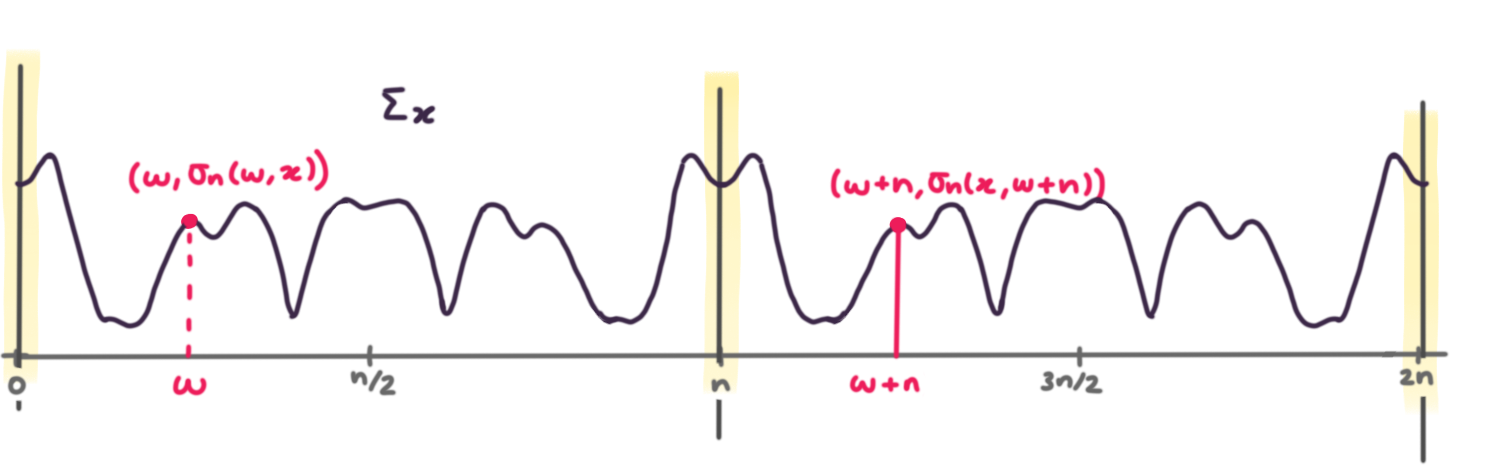
\includegraphics[scale = 0.9]{periodicidad_espectro} 
\end{figure}	


\subsection{Simetría}
\begin{prop}
\textbf{(Simetría de la función
\eqref{eq: estudiando espectro})}
Sean
$n \geq 2$,
$x \in \IR^{n}$. Para toda $0 \leq \omega \leq \frac{n}{2}$,
\[
\Sigma_{x}(\omega) = \Sigma_{x}(n-\omega).
\]
\end{prop}
\noindent
\textbf{Demostración.}
Debemos demostrar que se tiene la igualdad 
\[
\sigma_{n}(x, \omega) = 
\sigma_{n}(x, n-\omega ).
\]
En efecto, 
\begin{align*}
\tilde{c}_{n, \omega + n} = & \left( cos \left( 2 \pi
\left( n- \omega \right) \frac{m}{n} \right) \right)_{m=0}^{n-1} \\
= & \left( cos \left( 
2 \pi n \frac{m}{n} - 2 \pi \omega
\frac{m}{n}
\right) \right)_{m=0}^{n-1} \\
= & \left( cos \left( 
2 \pi m - 2 \pi \omega \frac{m}{n} 
\right) \right)_{m=0}^{n-1} \\
= & \left( cos \left( 2 \pi \omega \frac{m}{n} \right) \right)_{m=0}^{n-1}
= \tilde{c}_{n, \omega}
\end{align*}
y, similarmente,
\[
\tilde{s}_{n, \omega + Kn} = -\tilde{s}_{n, \omega};
\]
de esto, como en la demostración de la proposición
\ref{prop: periodicidad espectro}, se concluye la igualdad
entre los espacios $P_{n, \omega}$ y $P_{n, n-\omega}$, y de esto
la igualdad deseada.
\QEDB
\vspace{0.2cm}

\begin{figure}[H]
	\sidecaption{
	Podemos así afinar la afirmación hecha en la figura 
	\ref{fig: periodicidad espectro} y concluir que basta
	calcular los coeficientes
	$\sigma_{n}(x, \omega)$ para $0 \leq \omega \leq \frac{n}{2}$,
	pues los demás pueden deducirse a partir de reflexiones y traslaciones.
	\label{fig: simetria espectro}
	}
	\centering
	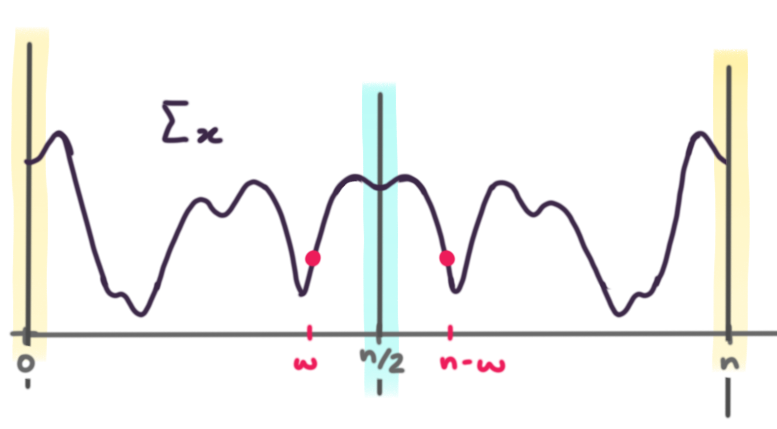
\includegraphics[scale = 1.4]{simetria_espectro} 
\end{figure}	
 

\begin{nota}
\label{nota: muestreo dom frecuencia}
Según estas propiedades de periodicidad y simetría,
podemos limitarnos a evaluar la función
$\Sigma_{x}$ sólo en frecuencias
contenidas en el intervalo $[0, n/2]$, pues los valores
del espectro para otros valores pueden deducirse por periodicidad
y simetría. \\

Ahora bien, para poder escribir programas
para calcular una tal función $\Sigma_{x}$,
se debe de usar como dominio de esta
un conjunto discreto de puntos.
Para los espectros que calcularemos de ahora en 
adelante, adoptamos la convención de 
usar usar como dominio 
de la función
$\Sigma_{x}$ de una señal $x \in \IR^{n}$
al conjunto
\begin{equation}
\label{eq: malla frecuencias}
\left\{ \frac{a}{100} : \hspace{0.2cm}
0 \leq a \leq 
\left\lfloor\frac{100n}{2}\right\rfloor,
\right\}
\end{equation}

\noindent
es decir, se toman $100$ muestras por
cada unidad del intervalo 
$\left[ 0, \frac{n}{2}\right]$
\end{nota}

\subsection{Continuidad}

Fijada una $n \geq 2$ y una $x \in \IR^{n}$,
vamos a analizar la continuidad de la función
$\Sigma_{x}$ como se definió 
en \eqref{eq: estudiando espectro}.
Por la periodicidad y simetría establecidas
en las proposiciones 
\TODO{ref}, basta
analizar la continuidad de $\Sigma_{x}$ sólo en el
intervalo cerrado $[0, n/2]$. Establecer la continuidad
de $\Sigma_{x}$ en el interior de este intervalo no es un problema. \\

\begin{prop}
Sean $n \geq 2$, $x \in \IR^{n}$,
$\Sigma_{x}$ como se definió en \eqref{eq: estudiando espectro}.
La función $\Sigma_{x}$ es continua en 
$]0, n/2[$
\end{prop}
\noindent
\textbf{Demostración.}
Sólo observe que la fórmula
\eqref{eq: coef sigma caso 1}, que sirve
para calcular el coeficiente $\sigma_{n} (x, \omega) = \Sigma_{x}(\omega)$
cuando $\omega \in ]0, n/2[$, es una combinación
de sumas y productos de senos y cosenos
evaluados en funciones de la frecuencia $\omega$, luego, 
es una función continua, por lo tanto $\Sigma_{x}$
es continua en el interior del intervalo 
$[0, n/2]$.
\QEDB
\vspace{0.2cm}

Sólo resta analizar la continuidad de 
$\Sigma_{x}$ en los puntos extremos $0$ y $n/2$.
Para ello,
será de utilidad introducir la siguiente notación.
\begin{defi}
\label{def: momentos de x}
Sean $n \geq 2$, $x= (x_{m})_{m=0}^{n-1} \in \IR^{n}$, $k \geq 0$.
Se definen a los números $M_{k}(x)$ y 
$\tilde{M}_{k}(x)$ como sigue;
	\begin{equation}
	\label{eq: momento k esimo de x}
	M_{k}(x) := \suma{m=0}{n-1}{m^{k}x_{m}}.
	\end{equation}
	
	\begin{equation}
	\label{eq: momento skew k esimo de x}
	\tilde{M}_{k}(x) := \suma{m=0}{n-1}{(-1)^{m}m^{k}x_{m}}.
	\end{equation}
\end{defi}


\begin{teo}
\label{teo: limite del espectro por cero}
Sean $n \geq 2$, $x \in \IR^{n}$.
Sea $\Sigma_{x}: [0, n/2] \rightarrow [0,1]$ 
como se definió en \eqref{eq: estudiando espectro}.
Se tiene que 
\begin{equation}
\label{eq: limite del espectro a cero}
\limite{\omega \rightarrow 0^{+}}{\Sigma_{x}(\omega)}
=
\left(
\frac{
2M_{0}(x)^{2}(2n-1)(n-1) + 12M_{1}(x)^{2} - 12M_{0}(x)M_{1}(x)(n-1)
}{
||x||^{2} (n-1)(n+1)n}
\right)^{1/2}
\end{equation}

y

\begin{equation}
\label{eq: limite del espectro a n medios}
\limite{\omega \rightarrow (n/2)^{-}}{\Sigma_{x}(\omega)}
= \left(
\frac{
2\tilde{M}_{0}(x)^{2}(2n-1)(n-1) + 12\tilde{M}_{1}(x)^{2} - 
12\tilde{M}_{0}(x)\tilde{M}_{1}(x)(n-1)
}{
||x||^{2} (n-1)(n+1)n}
\right)^{1/2}.
\end{equation}
\end{teo}
\noindent
\textbf{Demostración.}
Para calcular ambos límites, 
usaremos las series de Taylor
de las funciones seno y coseno alrededor del cero
con términos de hasta la potencia $5$ para aproximar
a los sinusoides que aparecen en la expresión 
\begin{equation}
\label{eq1: 22May}
\left(		  
		  \frac{\langle x, c_{n, \omega } \rangle^{2} +  \langle x, s_{n, \omega } \rangle^{2}	
	       -2  \langle x, c_{n, \omega } \rangle \langle x, s_{n, \omega } \rangle \langle c_{n, \omega }, s_{n, \omega } \rangle}{ || x ||^{2} \cdot
	       (1- \langle c_{n, \omega }, s_{n, \omega } \rangle^{2})}	  
\right) ^{1/2},
\end{equation}
es decir, usaremos
las siguientes aproximaciones, válidas en las cercanías
del cero;
\[
sen(\omega) 
\sim
\omega - \frac{\omega^{3}}{3!}
+ o(\omega^{5}),
\hspace{0.2cm} \omega \sim 0,
\]
\[
cos(\omega) \sim 1 - \frac{\omega^{2}}{2!}
+ \frac{\omega^{4}}{4!} + o(\omega^{5}),
\hspace{0.2cm} \omega \sim 0.
\]

Con estas aproximaciones, vamos a tener
a nuestra disposición expresiones como las siguientes;

\[
cos\left(
2 \pi \omega \frac{n-1}{n}\right) \sim
1-2\pi^{2}\frac{(n-1)^{2}}{n^{2}} \omega^{2}
+\frac{2}{3} \frac{(n-1)^{4}}{n^{4}} \pi^{4} \omega^{4}
+ o(\omega^{5}),
\]

\[
sen\left(
2 \pi \omega \frac{m}{n}\right) \sim
2 \pi \frac{m}{n} \omega 
- \frac{4}{3n^{3}}\pi^{3} \omega^{3}
+ o(\omega^{5}).
\]

Empecemos calculando 
el límite
\begin{equation}
\label{eq0: 22May}
\limite{\omega \rightarrow 0^{+}}{
\Sigma_{x}(\omega)}
= \limite{\omega \rightarrow 0^{+}}
{
\left(		  
		  \frac{\langle x, c_{n, \omega } \rangle^{2} +  \langle x, s_{n, \omega } \rangle^{2}	
	       -2  \langle x, c_{n, \omega } \rangle \langle x, s_{n, \omega } \rangle \langle c_{n, \omega }, s_{n, \omega } \rangle}{ || x ||^{2} \cdot
	       (1- \langle c_{n, \omega }, s_{n, \omega } \rangle^{2})}	  
\right) ^{1/2}
}.
\end{equation}


Usando las aproximaciones de las funciones seno y coseno
cerca del origen en 
las definiciones
\eqref{eq7: 19Marzo} y \eqref{eq8: 19Marzo}
de los factores de normalización
$\xi_{n, \omega}$ y $\eta_{n, \omega}$,
encontramos las siguientes aproximaciones,
válidas en las cercanías del cero.
 
\begin{align*}
\xi_{n, \omega} \sim &
\sqrt{2} 
\left(
4 \pi
\frac{                                                                                                                                          
\omega - \frac{2\pi^{2}}{3n^{2}}(2n^2-3n+2)\omega^{3} + o(\omega^{5})
}{
\frac{2\pi}{n} \omega -
\frac{4 \pi^{3}}{3 n^{3}} \omega^{3} + o(\omega^{5})
}
\right)^{-1/2} \\
\sim &
\sqrt{2} 
\left(
2n
\frac{                                                                                                                                          
\omega - \frac{2\pi^{2}}{3n^{2}}(2n^2-3n+2)\omega^{3} + o(\omega^{5})
}{
\omega -
\frac{2 \pi^{2}}{3 n^{2}} \omega^{3} + o(\omega^{5})
}
\right)^{-1/2} \\ &
\xrightarrow{\omega \rightarrow 0^{+}} 
\frac{1}{\sqrt{n}},
\end{align*}

\begin{align*}
\eta_{n, \omega} & \sim 
\sqrt{2} 
\left(
\frac{
8 \pi^{3} (2n-1)(n-1)\omega^{3} + o(\omega^{5})
}{
6 \pi n \omega -
\frac{4 \pi^{3}}{n} \omega^{3} + o(\omega^{5})
}
\right)^{-1/2} \\
& \sim 
\sqrt{2} 
\left(
4\pi^{2}
\frac{
(2n-1)(n-1)\omega^{3} + o(\omega^{5})
}{
3 n \omega -
\frac{2 \pi^{2}}{n} \omega^{3} + o(\omega^{5})
}
\right)^{-1/2}  \\  &
\xrightarrow{\omega \rightarrow 0^{+}} 
\infty.
\end{align*}
De la expresión para $\xi_{n, \omega}$ se calcula que

\noindent
\begin{align*}
\langle x,
c_{n, \omega}
\rangle = & 
\xi_{n, \omega} \langle x,
\tilde{c}_{n, \omega}
\rangle =  
\xi_{n, \omega} \suma{m=0}{n-1}{x_{m} cos \left(
2 \pi \omega \frac{m}{n}
\right)}
\\
\sim &
\xi_{n, \omega} 
\left(
M_{0}(x) - \frac{2 \pi^{2}}{n^{2}}X_{2} \omega^{2} 
+ \frac{2 \pi^{4}}{3n^{4}} M_{4}(x) \omega^{4} + o(\omega^{5})
\right) \\ &
\xrightarrow{\omega \rightarrow 0^{+}} \frac{M_{0}(x)}{\sqrt{n}}
. \\
\end{align*}

\noindent
Ahora bien, de la expresión para
$\eta_{n, \omega}$ se deduce la siguiente aproximación.

\begin{align*}
\langle x,
s_{n, \omega}
\rangle =
& 
\eta_{n, \omega} \langle x,
\tilde{s}_{n, \omega}
\rangle =  
\eta_{n, \omega} \suma{m=0}{n-1}{x_{m} sen \left(
2 \pi \omega \frac{m}{n}
\right)} \\
\sim &
\eta_{n, \omega}
\left(
\frac{2 \pi}{n} M_{1}(x) \omega - \frac{4 \pi^{3}}{3n^{3}}M_{3}(x) \omega^{3} 
 + o(\omega^{5})
\right)
\hspace{0.2cm}
\textit{cuando } \omega \sim 0
\\
\sim & 
\sqrt{2} 
\left(
\frac{
6 \pi n \omega -
\frac{4 \pi^{3}}{n} \omega^{3} + o(\omega^{5})
}{8 \pi^{3} (2n-1)(n-1)\omega^{3} + o(\omega^{5})
}
\right)^{1/2}
\cdot 
\left(
\frac{2 \pi}{n} M_{1}(x) \omega - \frac{4 \pi^{3}}{3n^{3}}M_{3}(x) \omega^{3} 
 + o(\omega^{5})
\right).
\end{align*}
Del intentar evaluar el límite de
$\langle x,
s_{n, \omega}
\rangle $ cuando $\omega \rightarrow 0^{+}$
con esta última aproximación asintótica se llega a una
indeterminación de tipo $\infty \cdot 0$.
Para desarrollar más esta última expresión para intentar
eliminar esta indeterminación, vamos a expresar 
el segundo factor 
\begin{equation}
\label{ec: seg factor}
\frac{2 \pi}{n} M_{1}(x) \omega - \frac{4 \pi^{3}}{3n^{3}}M_{3}(x) \omega^{3} 
 + o(\omega^{5})
\end{equation}
como la raíz cuadrada de su cuadrado.
Para hacer esto, deberemos de considerar el signo de este factor
\[
\frac{2 \pi}{n} M_{1}(x) \omega - \frac{4 \pi^{3}}{3n^{3}}M_{3}(x) \omega^{3} 
 + o(\omega^{5}) = 
 \frac{2\pi}{n} \omega \left(
 M_{1}(x) - \frac{2\pi^{2}}{3n^{2}}M_{3}(x)\omega^{2}
\right)
\]
que, por ser $\omega$ positivo, es el signo de 
\begin{equation}
\label{ec: seg factor 2}
M_{1}(x) - \frac{2\pi^{2}}{3n^{2}}M_{3}(x)\omega^{2}.
\end{equation}
Recuerde que en realidad sólo nos interesan valores de 
$\omega$ muy cercanos a cero (pues lo que queremos es evaluar
el límite de $\langle x, s_{n, \omega} \rangle$
cuando $\omega$ tiende a cero), luego, es posible escoger
un rango de $\omega$ de tal forma que el sumando 
$\frac{2\pi^{2}}{3n^{2}}M_{3}(x)\omega^{2}$ sea tan pequeño (comparado
con $M_{1}(x)$) que el signo de la expresión
\eqref{ec: seg factor 2}
(i.e. el de \eqref{ec: seg factor}) sea 
el de $M_{1}(x)$. Si
\begin{align*}
sgn(M_{1}(x))= \begin{cases}
1 & \hspace{0.2cm} \textit{ si } M_{1}(x) \geq 0, \\
-1 & \hspace{0.2cm} \textit{ si } M_{1}(x) < 0,
\end{cases}
\end{align*}

\noindent
podemos entonces seguir la cadena de
aproximaciones asintóticas de $\langle x, s_{n, \omega} \rangle$ 
como sigue.

\begin{align*}
\langle x,
s_{n, \omega}
\rangle \sim &
sgn(M_{1}(x))
\sqrt{2} 
\left(
\frac{
6 \pi n \omega -
\frac{4 \pi^{3}}{n} \omega^{3} + o(\omega^{5})
}{8 \pi^{3} (2n-1)(n-1)\omega^{3} + o(\omega^{5})
}
\right)^{1/2}
\cdot 
\left(
\left(
\frac{2 \pi}{n} M_{1}(x) \omega - \frac{4 \pi^{3}}{3n^{3}}M_{3}(x) \omega^{3} 
 + o(\omega^{5})
\right)^{2}
\right)^{1/2}\\
= & 
sgn(M_{1}(x)) \sqrt{2} \left(
\frac{
\frac{24 \pi^{3}}{n}X_{1}^{2}\omega^{3} + o(\omega^{5}) }{
8 \pi^{3} (2n-1)(n-1)\omega^{3} + o(\omega^{5})
}
\right)^{1/2} \\
\xrightarrow{\tilde{\omega} \rightarrow 0^{+}}& sgn(M_{1}(x))\left(
\frac{6 M_{1}(x)^{2}}{(2n-1)(n-1)n}
\right)^{1/2} 
= M_{1}(x) 
\left(
\frac{6 }{(2n-1)(n-1)n}
\right)^{1/2} 
\end{align*}
Por último, encontremos un equivalente
asintótico, válido en las cercanías de $0$, de 
$\langle
c_{n, \omega}, s_{n, \omega}
\rangle $.
\begin{align*}
\langle
c_{n, \omega}, s_{n, \omega}
\rangle = &
\xi_{n, \omega} \eta_{n, \omega}
\suma{m=0}{n-1}{
cos\left(
2 \pi \omega\frac{m}{n}
\right)
sen\left(
2 \pi \omega\frac{m}{n}
\right)
} \\
\sim &
\frac{2\pi}{n}
\xi_{n, \omega} \eta_{n, \omega}
(n-1)  
\left(
\frac{n}{2} \omega - \frac{2\pi^{2}}{3} (n-1) \omega^{3} + o(\omega^{5})
\right) 
\hspace{0.2cm} \textit{ cuando } \omega \sim 0
\\
\sim &
\frac{2\pi}{n \sqrt{n}}
(n-1) 
\eta_{n, \omega} 
\left(
\frac{n}{2} \omega - \frac{2\pi^{2}}{3} (n-1) \omega^{3} + o(\omega^{5})
\right). \\
\end{align*}
Nuevamente, el factor 
$\eta_{n, \omega}$, que tiende a $\infty$
conforme $\omega \rightarrow 0^{+}$,
nos hace tener una indeterminación
del tipo $\infty \cdot 0$
cuando intentamos calcular el límite
de 
$
\limite{\omega \rightarrow 0^{+}}{
\langle
c_{n, \omega}, s_{n, \omega}
\rangle}
$.
Observe que, puesto que sólo nos interesan los valores
de $\omega$ cercanos a cero, el factor 
$
\frac{n}{2} \omega - \frac{2\pi^{2}}{3} (n-1) \omega^{3} + o(\omega^{5})
$
es positivo 
para $\omega$ lo suficientemente pequeño
(pues siempre es posible encontrar una cota
superior para $\omega$, cercana a cero, de tal forma que se 
cumpla la desigualdad $\frac{n}{2} \geq \frac{2 \pi^{2}}{3}(n-1)
\omega^{2}$ para las frecuencias $\omega$ menores a tal cota), luego, 
en este caso podemos proceder sin problemas a expresar este
factor
como la raíz cuadrada de su cuadrado, para poder concluir lo siguiente; 


\begin{align*}
\langle
c_{n, \omega}, s_{n, \omega}
\rangle \sim & 
\frac{2 \sqrt{2}}{n \sqrt{n}} \pi (n-1)
\left(
\frac{
\frac{3}{2} \pi n^{3}\omega^{3} + o(\omega^{5})
}{
8 \pi^{3}(2n-1)(n-1)\omega^{3} + o(\omega^{5})
}
\right)^{1/2} 
\hspace{0.2cm} \textit{ cuando } \omega \sim 0
\\
\xrightarrow{\omega \rightarrow 0^{+}} & \frac{
\sqrt{6(n-1)}
}{2 \sqrt{2n-1}}.
\end{align*} 

De estos límites se deduce que 

\begin{equation}
\label{ec: limite x, cnw cuadr}
\limite{\omega \rightarrow 0^{+}}{\langle
x, c_{n, \omega}
\rangle^{2} }
= \frac{M_{0}(x)^{2}}{n},
\end{equation}
\begin{equation}
\label{ec: limite x, snw cuad}
\limite{\omega \rightarrow 0^{+}}{\langle
x, s_{n, \omega}
\rangle^{2} }
= \frac{6M_{1}(x)^{2}}{(2n-1)(n-1)n},
\end{equation}

\begin{align}
\label{ec: limite -2abc}
\limite{\omega \rightarrow 0^{+}}{
-2 \langle x, c_{n, \omega} \rangle
\langle x, s_{n, \omega} \rangle
\langle c_{n, \omega}, s_{n, \omega} \rangle} = &
-2 
\frac{M_{0}(x)}{\sqrt{n}} \cdot 
\frac{M_{1}(x) \sqrt{6}}{\sqrt(n(n-1)(2n-1)} \cdot
\frac{\sqrt{6} \sqrt{n-1}}{\sqrt{2n-1}} \nonumber \\
= &
-\frac{6 M_{0}M_{1}(x)}{n(2n-1)},
\end{align}
\begin{equation}
\label{ec: limite cnw, snw cuad aa}
\limite{\omega \rightarrow 0^{+}}{\langle
c_{n, \omega}, s_{n, \omega}
\rangle^{2} }
= \frac{3(n-1)}{2(2n-1)}.
\end{equation}
Observe que $1-\frac{3(n-1)}{2(2n-1)}$
nunca es cero, o sea, que sustituyendo la 
expresión \eqref{ec: limite cnw, snw cuad aa}
en 
\eqref{eq1: 22May}
no se tiene un denominador igual a cero, por lo que podemos
sustituir los límites
\eqref{ec: limite x, cnw cuadr},
\eqref{ec: limite x, snw cuad},
\eqref{ec: limite -2abc} y
\eqref{ec: limite cnw, snw cuad aa}
en \eqref{eq1: 22May}
y concluir que el límite buscado
\eqref{eq0: 22May} existe y es igual
\begin{align*}
\limite{\omega \rightarrow 0^{+}}{\Sigma_{x}(\omega)}
= & 
\left(
\frac{
\frac{M_{0}(x)^{2}}{n} + \frac{6M_{1}(x)^{2}}{n(2n-1)(n-1)}
- \frac{6 M_{0}(x) M_{1}(x)}{n(2n-1)}
}{
||x||^{2} \left(
1- 1.5 \frac{n-1}{2n-1}
\right)
}
\right)^{1/2} \\
= &
\frac{
2M_{0}(x)^{2}(2n-1)(n-1) + 12M_{1}(x)^{2} - 12M_{0}(x)M_{1}(x)(n-1)
}{
||x||^{2} (n-1)(n+1)n.
}
\end{align*}


Determinemos ahora el límite de
\eqref{eq1: 22May} cuando $\omega \rightarrow (n/2)^{-}$.
Para aprovechar todo lo calculado antes, vamos a hacer
el cambio de variable 
\[
\omega = \frac{n}{2} - \tilde{w},
\]
pues $\omega \rightarrow (n/2)^{-}$ si y sólo si
$\tilde{\omega} \rightarrow 0^{+}$.


Se calcula que 
\[
cos\left(
2 \pi \omega\frac{n-1}{n}
\right) = (-1)^{n-1} cos\left(
2 \pi \tilde{\omega}\frac{n-1}{n}
\right), \hspace{0.2cm}
cos\left(
2 \pi \omega\frac{m}{n}
\right) = (-1)^{m} cos\left(
2 \pi \tilde{\omega}\frac{m}{n}
\right), 
\]
\[
cos\left(
2 \pi \frac{\omega}{n}
\right) = -cos\left(
2 \pi \frac{\tilde{\omega}}{n}
\right), 
\]


\[
sen \left( 2 \pi \omega \right)
= (-1)^{n-1} sen (2 \pi \tilde{\omega})
, \hspace{0.2cm}
sen\left(
2 \pi \omega\frac{m}{n}
\right) = (-1)^{m+1} sen\left(
2 \pi \tilde{\omega}\frac{m}{n}
\right), 
\]
\[
sen\left(
2 \pi \frac{\omega}{n}
\right) = sen\left(
2 \pi \frac{\tilde{\omega}}{n}
\right).
\]

De usar las definiciones
de $\xi_{n, \omega}$ y $\eta_{n, \omega}$
y las relaciones anteriores entre senos y cosenos
de ángulos que involucran a $\omega$ y $\tilde{\omega}$
se sigue de inmediato que
\[
\xi_{n, \omega} = \xi_{n, \tilde{\omega}}
\hspace{0.2cm} \textit{ y } \hspace{0.2cm}
\eta_{n, \omega} = \eta_{n, \tilde{\omega}},
\]
luego, 

\begin{align*}
\xi_{n, \omega} = &
\xi_{n, \tilde{\omega}} \\
\sim &
\sqrt{2} 
\left(
2n
\frac{                                                                                                                                          
\tilde{\omega} - \frac{2\pi^{2}}{3n^{2}}(2n^2-3n+2)\tilde{\omega}^{3} 
+ o(\tilde{\omega}^{5})
}{
\tilde{\omega} -
\frac{2 \pi^{2}}{3 n^{2}} \tilde{\omega}^{3} + o(\tilde{\omega}^{5})
}
\right)^{-1/2}
\hspace{0.2cm} \textit{ cuando } \tilde{\omega} \sim 0
\\ &
\xrightarrow{\tilde{\omega} \rightarrow 0^{+}} 
\frac{1}{\sqrt{n}},
\end{align*}
y 
\begin{align*}
\eta_{n, \omega} = &
\eta_{n, \tilde{\omega}} \\
& \sim 
\sqrt{2} 
\left(
4\pi^{2}
\frac{
(2n-1)(n-1)\tilde{\omega}^{3} + o(\tilde{\omega}^{5})
}{
3 n \tilde{\omega} -
\frac{2 \pi^{2}}{n} \tilde{\omega}^{3} + o(\tilde{\omega}^{5})
}
\right)^{-1/2}  
\hspace{0.2cm} \textit{ cuando } \tilde{\omega} \sim 0
\\  &
\xrightarrow{\tilde{\omega} \rightarrow 0^{+}} 
\infty.
\end{align*}
Tenemos entonces que
\[
\limite{\omega \rightarrow (n/2)^{-}}{
\xi_{n, \omega}} = \frac{1}{\sqrt{n}},
\hspace{0.2cm}
\limite{\omega \rightarrow (n/2)^{-}}{
\eta_{n, \omega}} = \infty.
\]

De forma análoga pueden reutilizarse los cálculos anteriores,
cambiando los factores $M_{k}(x)$ por los $\tilde{M}_{k}(x)$
para deducir los siguientes límites.


\begin{align*}
\langle x,
c_{n, \omega}
\rangle = & 
\xi_{n, \omega} \langle x,
\tilde{c}_{n, \omega}
\rangle =  
\xi_{n, \omega} \suma{m=0}{n-1}{x_{m} cos \left(
2 \pi \omega \frac{m}{n}
\right)}
\\
= &  
\xi_{n, \tilde{\omega}} \suma{m=0}{n-1}{(-1)^{m}x_{m} cos \left(
2 \pi \tilde{\omega} \frac{m}{n}
\right)}\\
\sim &
\xi_{n, \tilde{\omega}} 
\left(
\tilde{M}_{0}(x) - \frac{2 \pi^{2}}{n^{2}}\tilde{M}_{2} \tilde{\omega}^{2} 
+ \frac{2 \pi^{4}}{3n^{4}} \tilde{M}_{4}(x) \tilde{\omega}^{4} + o(\tilde{\omega}^{5})
\right) 
\hspace{0.2cm} \textit{ cuando } \tilde{\omega} \sim 0
\\
& 
\xrightarrow{\tilde{\omega} \rightarrow 0^{+}}
\frac{\tilde{M}_{0}(x)}{\sqrt{n}},
\end{align*}

\begin{align*}
\langle x,
s_{n, \omega}
\rangle = &
\eta_{n, \omega}
\langle
x, \tilde{s}_{n, \omega}
\rangle
= \eta_{n, \omega}
\suma{m=0}{n-1}{
x_{m}sen\left(
2 \pi \omega\frac{m}{n}
\right)
} \\
= &
- \eta_{n, \tilde{\omega}}
\suma{m=0}{n-1}{
(-1)^{m}
x_{m}sen\left(
2 \pi \tilde{\omega} \frac{m}{n}
\right)
} \\
\sim &
-\eta_{n, \tilde{\omega}}
\left(
\frac{2\pi}{n} \tilde{M}_{1}(x)\tilde{\omega}
-\frac{4\pi^{3}}{3n^{3}} \tilde{M}_{3}(x)\tilde{\omega}^{3}
+ o(\tilde{\omega}^{5})
\right)
\hspace{0.2cm} \textit{ cuando } \tilde{\omega} \sim 0 \\
\sim &
- sgn(\tilde{M}_{1}(x))
\sqrt{2} 
\left(
\frac{
6 \pi n \tilde{\omega} -
\frac{4 \pi^{3}}{n} \tilde{\omega}^{3} + o(\tilde{\omega}^{5})
}{8 \pi^{3} (2n-1)(n-1)\tilde{\omega}^{3} + o(\tilde{\omega}^{5})
}
\right)^{1/2}
\cdot 
\left(
\left(
\frac{2 \pi}{n} \tilde{M}_{1}(x) \tilde{\omega} - \frac{4 \pi^{3}}{3n^{3}}
\tilde{M}_{3}(x) \tilde{\omega}^{3} 
 + o(\tilde{\omega}^{5})
\right)^{2}
\right)^{1/2}\\
\xrightarrow{\tilde{\omega} \rightarrow 0^{+}} & - 
sgn(\tilde{M}_{1}(x))
\left(
\frac{6 \tilde{M}_{1}(x)^{2}}{(2n-1)(n-1)n}
\right)^{1/2}
= -M_{1}(x)
\left(
\frac{6}{(2n-1)(n-1)n}
\right)^{1/2}
\end{align*}

Por último, 

\begin{align*}
\langle
c_{n, \omega}, s_{n, \omega}
\rangle = &
\xi_{n, \omega} \eta_{n, \omega}
\suma{m=0}{n-1}{
cos\left(
2 \pi \omega\frac{m}{n}
\right)
sen\left(
2 \pi \omega\frac{m}{n}
\right)
} \\
= &
\xi_{n, \tilde{\omega}} \eta_{n, \tilde{\omega}}
\suma{m=0}{n-1}{
(-1)^{m}cos\left(
2 \pi \tilde{\omega} \frac{m}{n}
\right) \cdot (-1)^{m+1}
sen\left(
2 \pi \tilde{\omega} \frac{m}{n}
\right)
}
\\
= &
-\xi_{n, \tilde{\omega}} \eta_{n, \tilde{\omega}}
\suma{m=0}{n-1}{
cos\left(
2 \pi \tilde{\omega}\frac{m}{n}
\right) 
sen\left(
2 \pi \tilde{\omega}\frac{m}{n}
\right)
}
\\
\xrightarrow{\tilde{\omega} \rightarrow 0^{+}}&
- \frac{\sqrt{6(n-1)}}{2 \sqrt{2n-1}}.
\end{align*}

Así,
\begin{align*}
-2 \langle x, c_{n, \omega} \rangle
\langle x, s_{n, \omega} \rangle
\langle c_{n, \omega}, s_{n, \omega} \rangle & \\
\xrightarrow{\tilde{\omega} \rightarrow 0^{+}} & 
-2 \frac{\tilde{M}_{0}(x)}{\sqrt{n}}
\cdot 
(-1) \tilde{M}_{1}(x)\frac{\sqrt{6}}{
\sqrt{(2n-1)(n-1)n}}
\cdot (-1)
\frac{\sqrt{6(n-1)}}{2 \sqrt{2n-1}}
\\
= & - \frac{6 \tilde{M}_{0}(x)\tilde{M}_{1}(x)}{n(2n-1)}.
\end{align*}



Obtenemos así los siguientes límites.
\begin{equation}
\label{ec: limite x, cnw cuadr n med}
\limite{\omega \rightarrow (n/2)^{-}}{\langle
x, c_{n, \omega}
\rangle^{2} }
= \frac{\tilde{M}_{0}(x)^{2}}{n},
\end{equation}
\begin{equation}
\label{ec: limite x, snw cuad n med}
\limite{\omega \rightarrow (n/2)^{-}}{\langle
x, s_{n, \omega}
\rangle^{2} }
= \frac{6\tilde{M}_{1}(x)^{2}}{(2n-1)(n-1)n},
\end{equation}

\begin{equation}
\label{ec: limite -2abc n med}
\limite{\omega \rightarrow (n/2)^{-}}{
-2 \langle x, c_{n, \omega} \rangle
\langle x, s_{n, \omega} \rangle
\langle c_{n, \omega}, s_{n, \omega} \rangle
= 
- \frac{6\tilde{M}_{0}(x)\tilde{M}_{1}(x)}{n(2n-1)},
}
\end{equation}
\begin{equation}
\label{ec: limite cnw, snw cuad}
\limite{\omega \rightarrow (n/2)^{-}}{\langle
c_{n, \omega}, s_{n, \omega}
\rangle^{2} }
= \frac{3(n-1)}{2(2n-1)}.
\end{equation}
De nuevo no hay problemas de indeterminación al 
sustituir \eqref{ec: limite cnw, snw cuad} en 
\eqref{eq1: 22May}, por lo que podemos 
sustituir 
\eqref{ec: limite x, cnw cuadr n med}, 
\eqref{ec: limite x, snw cuad n med}, 
\eqref{ec: limite -2abc n med} y 
\eqref{ec: limite cnw, snw cuad} en 
\eqref{eq1: 22May} para concluir que el límite por la izquierda
de $n/2$ del espectro $\Sigma_{x}$ es, en efecto,
el propuesto
en 
\eqref{eq: limite del espectro a cero}. \\
\QEDB
\vspace{0.2cm}


Con unos ejemplos,
fijando a una señal $x$,
es fácil comprobar que los límites extremos 
\eqref{eq: limite del espectro a cero} y 
\eqref{eq: limite del espectro a n medios}
no siempre coinciden con los valores
de la función $\Sigma_{x}$ en tales extremos.


%\section{PROVISIONAL; límites}

En \TODO{rojo} se resaltan las fórmulas que YA se han
verificado calculándolas dos veces. En 
\textcolor{blue}{azul} cuando la aproximación ha sido
simulada exitosamente.


\TODO{
\[
\frac{sen(2 \pi \omega) cos(2 \pi \omega \frac{n-1}{n})}{sen
(2 \pi \frac{\omega}{n})}
\sim
\frac{
2 \pi \omega - \frac{4 \pi^{3}}{3n^{2}}
(4n^2-6n+3) \omega^{3} + o(\omega^{5})
}{
\frac{2\pi}{n} \omega -
\frac{4 \pi^{3}}{3 n^{3}} \omega^{3} + o(\omega^{5})
},
\]
}
por lo que

\textcolor{blue}{
\begin{align*}
\xi_{n, \omega} \sim &
\sqrt{2} 
\left(
4 \pi
\frac{                                                                                                                                          
\omega - \frac{2\pi^{2}}{3n^{2}}(2n^2-3n+2)\omega^{3} + o(\omega^{5})
}{
\frac{2\pi}{n} \omega -
\frac{4 \pi^{3}}{3 n^{3}} \omega^{3} + o(\omega^{5})
}
\right)^{-1/2} \\
\sim &
\sqrt{2} 
\left(
2n
\frac{                                                                                                                                          
\omega - \frac{2\pi^{2}}{3n^{2}}(2n^2-3n+2)\omega^{3} + o(\omega^{5})
}{
\omega -
\frac{2 \pi^{2}}{3 n^{2}} \omega^{3} + o(\omega^{5})
}
\right)^{-1/2} 
\rightarrow \frac{1}{\sqrt{n}},
\end{align*}
}

\textcolor{blue}{
\begin{align*}
\eta_{n, \omega} \sim &
\sqrt{2} 
\left(
\frac{
8 \pi^{3} (2n-1)(n-1)\omega^{3} + o(\omega^{5})
}{
6 \pi n \omega -
\frac{4 \pi^{3}}{n} \omega^{3} + o(\omega^{5})
}
\right)^{-1/2} \\
\sim & 
\sqrt{2} 
\left(
4\pi^{2}
\frac{
(2n-1)(n-1)\omega^{3} + o(\omega^{5})
}{
3 n \omega -
\frac{2 \pi^{2}}{n} \omega^{3} + o(\omega^{5})
}
\right)^{-1/2} 
 \rightarrow \infty.
\end{align*}
}

\textcolor{blue}{
\begin{align*}
\langle
c_{n, \omega}, s_{n, \omega}
\rangle \sim &
\frac{2\pi}{n}
\xi_{n, \omega} \eta_{n, \omega}
(n-1)  
\left(
\frac{n}{2} \omega - \frac{2\pi^{2}}{3} (n-1) \omega^{3} + o(\omega^{5})
\right) \\
= & 
\frac{2 \sqrt{2}}{n \sqrt{n}} \pi (n-1)
\left(
\frac{
\frac{3}{2} \pi n^{3}\omega^{3} + o(\omega^{5})
}{
8 \pi^{3}(2n-1)(n-1)\omega^{3} + o(\omega^{5})
}
\right)^{1/2}
\rightarrow \frac{
\sqrt{6(n-1)}
}{2 \sqrt{2n-1}}.
\end{align*} 
}
Tuve que usar la expresión asintótica
de $\eta_{n, \omega}$ para poder determinar este
último límite, pues con la expresión de la
primera linea tenía una indeterminación
de tipo $\infty \cdot 0$.

\textcolor{blue}{
\[
\langle x,
c_{n, \omega}
\rangle = 
\xi_{n, \omega} 
\left(
X_{0} - \frac{2 \pi^{2}}{n^{2}}X_{2} \omega^{2} 
+ \frac{2 \pi^{4}}{3n^{4}} X_{4} \omega^{4} + o(\omega^{5})
\right) \rightarrow \frac{X_{0}}{\sqrt{n}} ,
\]
}

\textcolor{blue}{
\begin{align*}
\langle x,
s_{n, \omega}
\rangle = &
\eta_{n, \omega} 
\left(
\frac{2 \pi}{n} X_{1} \omega - \frac{4 \pi^{3}}{3n^{3}}X_{3} \omega^{3} 
 + o(\omega^{5})
\right)\\
= &
\begin{cases}
\sqrt{2} \left(
\frac{
\frac{24 \pi^{3}}{n}X_{1}^{2}\omega^{3} + o(\omega^{5}) }{
8 \pi^{3} (2n-1)(n-1)\omega^{3} + o(\omega^{5})
}
\right)^{1/2}
\rightarrow \left(
\frac{6 X_{1}^{2}}{(2n-1)(n-1)n}
\right)^{1/2} & \textit{si } \alpha_{n, \omega}(x) \geq 0 \\
-\sqrt{2} \left(
\frac{
\frac{24 \pi^{3}}{n}X_{1}^{2}\omega^{3} + o(\omega^{5}) }{
8 \pi^{3} (2n-1)(n-1)\omega^{3} + o(\omega^{5})
}
\right)^{1/2}
\rightarrow -\left(
\frac{6 X_{1}^{2}}{(2n-1)(n-1)n}
\right)^{1/2} & \textit{si } \alpha_{n, \omega}(x) < 0,\\
\end{cases}
\end{align*}
}
donde
\[
\alpha_{n, \omega}(x) := 
\frac{2 \pi}{n} X_{1} \omega - \frac{4 \pi^{3}}{3n^{3}}X_{3} \omega^{3}.
\] 

\TODO{Ya lo tengo. Lo único no tan lindo de la fórmula
es que se requiere calcular el signo del coeficiente alpha. No sé si 
sea siempre fácil de determinar-o si quiera
si sea constante cerca de cero. Lo que yo hice en el programa es determiar
el signo para cuando $\omega = 0.001$}





\begin{equation}
\label{ec: limite x, cnw}
\limite{\omega \rightarrow 0^{+}}{\langle
x, c_{n, \omega}
\rangle }
= \frac{X_{0}}{\sqrt{n}}
\end{equation}

\begin{equation}
\label{ec: limite x, snw}
\limite{\omega \rightarrow 0^{+}}{\langle
x, s_{n, \omega}
\rangle }
\begin{cases}
\left(
\frac{6 X_{1}^{2}}{(2n-1)(n-1)n}
\right)^{1/2} & \textit{si } \alpha_{n, \omega}(x) \geq 0 \\
-\left(
\frac{6 X_{1}^{2}}{(2n-1)(n-1)n}
\right)^{1/2} & \textit{si } \alpha_{n, \omega}(x) < 0,\\
\end{cases}
\end{equation}

\begin{equation}
\label{ec: limite -2abc}
\limite{\omega \rightarrow 0^{+}}{
-2 \langle x, c_{n, \omega} \rangle
\langle x, s_{n, \omega} \rangle
\langle c_{n, \omega}, s_{n, \omega} \rangle
= 
}
\end{equation}

Así, los elementos que parecen en la fórmula
para $\sigma_{n}(x, \omega)$ cuando $\omega \not\in \frac{n}{2} \IZ$ son
\begin{itemize}
\item 
\TODO{
\[
\langle
c_{n, \omega}, s_{n, \omega}
\rangle^{2} \sim
\frac{4\pi^{2}}{n^{2}}(n-1)^{2} \xi_{n, \omega}^{2} \eta_{n, \omega}^{2}
\left(
\frac{n^{2}}{4} \omega^{2} - \frac{2n}{3} \pi^{2} (n-1) \omega^{4} + o(\omega^{5})
\right)
\]
}
sigue desarrollando el eta  !!!
\item
\TODO{
\[
\langle x,
c_{n, \omega}
\rangle^{2} = 
\xi_{n, \omega}^{2}
\left(
X_{0}^{2} - \frac{4 \pi^{2}}{n^{2}}X_{0}X_{2} \omega^{2} 
+ 
\frac{4 \pi^{4}}{n^{4}}
\left(
\frac{1}{3} X_{0}X_{4} + X_{2}^{2}
\right) \omega^{4} 
+ o(\omega^{5})
\right)
\]
}

\item
\TODO{
\[
\langle x,
s_{n, \omega}
\rangle^{2} = 
\frac{4 \pi^{2}}{n^{2}}
\eta_{n, \omega}^{2}
\left(
X_{1}^{2}\omega^{2} - \frac{4 \pi^{2}}{3n^{2}}X_{1}X_{3} \omega^{4} 
+  o(\omega^{5})
\right)
\]
}

\item
\[
\langle
x, c_{n, \omega}
\rangle
\langle
x, s_{n, \omega}
\rangle
\langle
c_{n, \omega}, s_{n, \omega}
\rangle \sim
\frac{2 \pi^{2}}{n}
\xi_{n, \omega}^{2} \eta_{n, \omega}^{2}(n-1)
\left(
X_{0}X_{1}\omega^{2} 
- \frac{2 \pi^{2}}{n}
\left(
\frac{1}{3n} X_{0}X_{3} + \frac{1}{n} X_{2}X_{1}
+ \frac{2}{3}(n-1)X_{0}X_{1}
\right) \omega^{4}
\right).
\]
\end{itemize}

\TODO{Cambia los iguales por $\sim$.}
Según estos cálculos, si
$a_{n, \omega} = \langle x, c_{n, \omega} \rangle$, 
$b_{n, \omega} = \langle x, s_{n, \omega} \rangle$, 
$c_{n, \omega} = \langle c_{n, \omega}, s_{n, \omega} \rangle$, 
entonces

\[
a_{n, \omega}^{2} + b_{n, \omega}^{2} - 
2a_{n, \omega}b_{n, \omega}c_{n, \omega}
= N_{1} + N_{2} +N_{3},
\]
donde

\[
N_{1} =
\xi_{n, \omega}^{2} \left(
X_{0}^{2} - \frac{4\pi^{2}}{n^{2}} X_{0}X_{2}
\omega^{2} + \frac{4 \pi^{4}}{n^{4}}
\left(
\frac{1}{3} X_{0}X_{4} + X_{2}^{2}
\right) \omega^{4}
\right)
\rightarrow 
\frac{X_{0}}{n}
\left(
X_{0}  - \frac{4 \pi^{2}}{n^{2}}X_{2}
\right),
\]

\[
N_{2} = \frac{4 \pi^{2}}{n^{2}} \eta_{n, \omega}^{2}
\left(
X_{1}^{2} \omega^{2} - \frac{4 \pi^{2}}{3n^{2}}X_{1}X_{3} \omega^{4}
+ o(\omega^{5})
\right)
=
\frac{16 \pi^{3}}{n^{2}}
\frac{3n \omega - \frac{2 \pi^{2}}{n} \omega^{3} + o(\omega^{5})}{
8 \pi^{3}(2n-1)(n-1) \omega^{3} + o(\omega^{5})
}
\rightarrow \infty,
\]

\[
N_{3} =
\frac{-4 \pi^{2}}{n}
\xi_{n, \omega}^{2} \eta_{n, \omega}^{2}(n-1)
\left(
X_{0}X_{1}\omega^{2} 
- \frac{2 \pi^{2}}{n}
\left(
\frac{1}{3n} X_{0}X_{3} + \frac{1}{n} X_{2}X_{1}
+ \frac{2}{3}(n-1)X_{0}X_{1}
\right) \omega^{4}
\right)
\rightarrow ?,
\]
luego, no puedo determinar este último límite, por lo tanto,
tampoco hablar solbre el límite de
de $a_{n, \omega}^{2} + b_{n, \omega}^{2} - 
2a_{n, \omega}b_{n, \omega}c_{n, \omega}$, pues
tengo una indeterminación del tipo 
$0 \cdot \infty$. \\

El denominador es
\[
1-c^{2} \sim
1 - \frac{4\pi^{2}}{n^{2}}(n-1)^{2} \xi_{n, \omega}^{2} \eta_{n, \omega}^{2}
\left(
\frac{n^{2}}{4} \omega^{2} - \frac{2n}{3} \pi^{2} (n-1) \omega^{4} + o(\omega^{5})
\right) \rightarrow ?,
\]
aquí también tengo una indeterminación de tipo
$0 \cdot \infty$. aquí están algunos resultados en limpio (sin desarrollo) de lo que calculé para poder determinar los límites extremos del espectro de una señal.

\begin{figure}[H]
	\sidecaption{
	Se grafica el espectro del PDL
	$\cali{L}^{12,1}$. Observe que el espectro
	es continuo por la derecha de $6$, pero tiene
	una discontinuidad de salto a la izquierda de $0$.
	\label{fig: lim 1}
	}
	\centering
	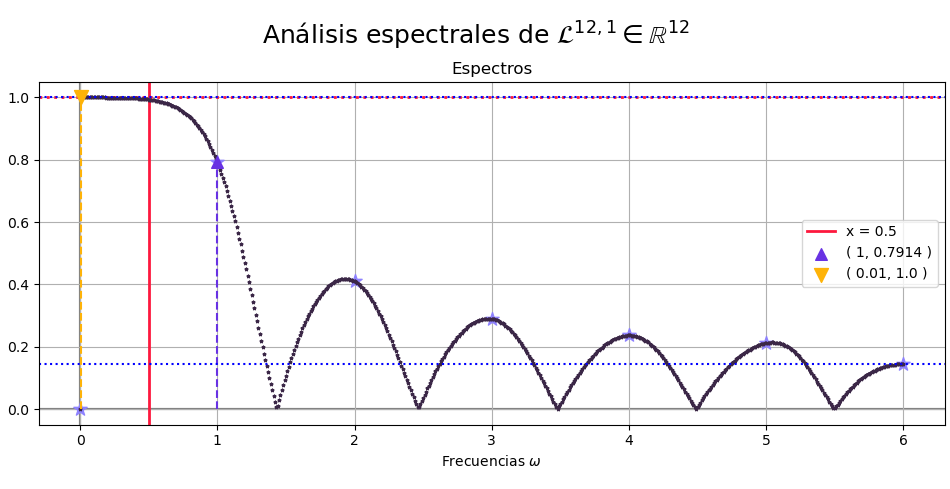
\includegraphics[scale = 0.5]{lim_1} 
\end{figure}	

\begin{figure}[H]
	\sidecaption{
	Observe que el espectro de $\cali{L}^{12,8}$ es, por el 
	contrario, continuo por $0$ pero discontinuo por $6$.
	\label{fig: lim 2}
	}
	\centering
	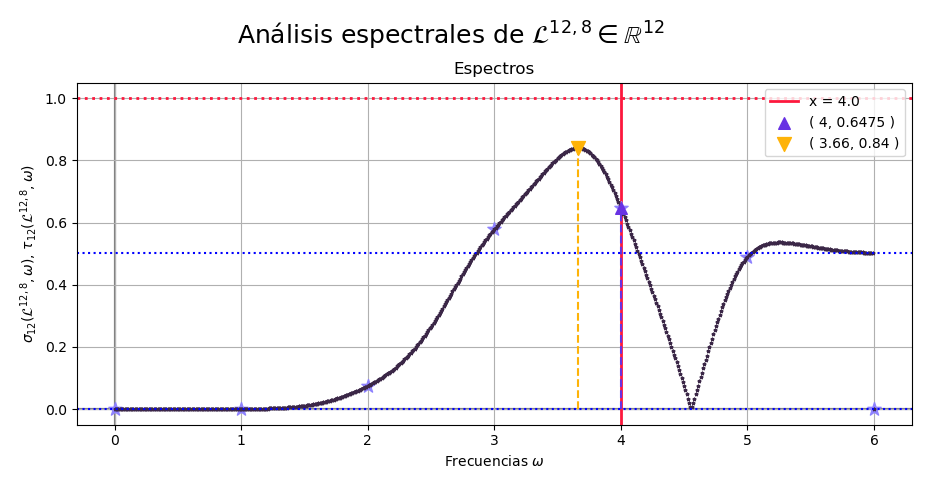
\includegraphics[scale = 0.5]{lim_2} 
\end{figure}

\begin{figure}[H]
	\sidecaption{
	El espectro de $\cali{L}^{12,9}$ es
	continuo por ambos extremos $0$ y $6$.
	\label{fig: lim 2}
	}
	\centering
	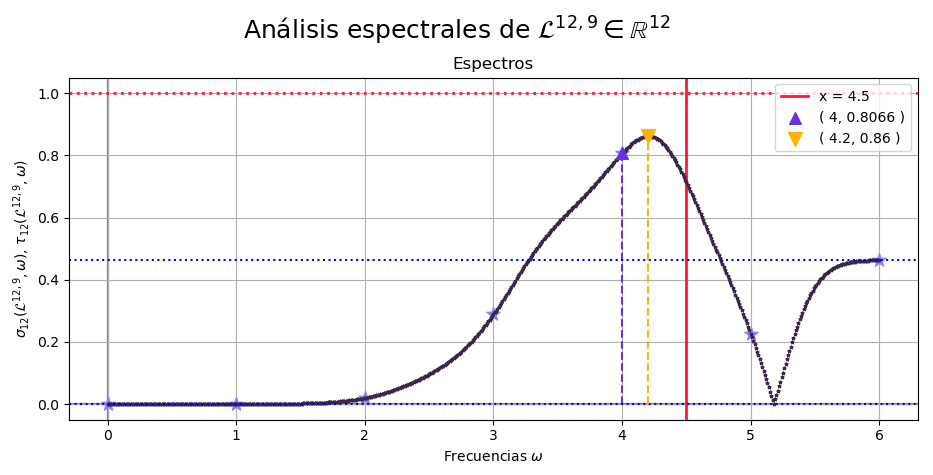
\includegraphics[scale = 0.5]{lim_3} 
\end{figure}

\begin{figure}[H]
	\sidecaption{
	El espectro de la señal
	$x = (1, 2, -3, -6) \in \IR^{4}$
	es discontinuo por ambos extremos
	$0$ y $2$.
	\label{fig: lim 4}
	}
	\centering
	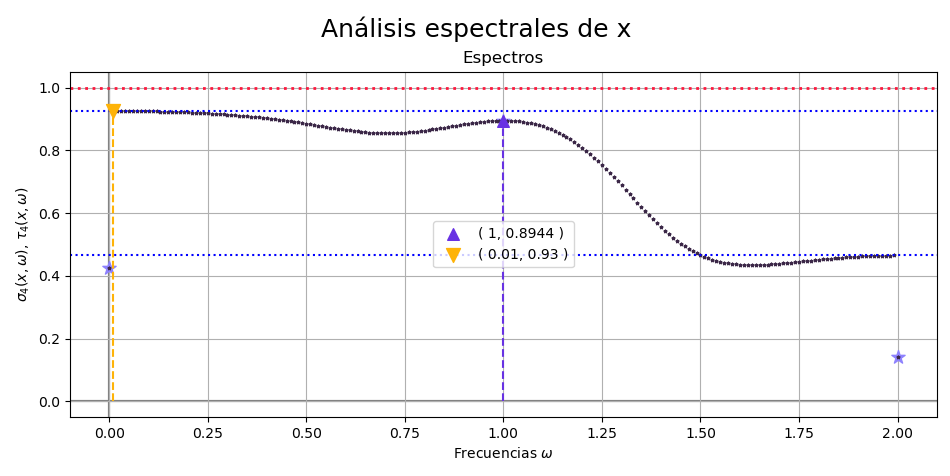
\includegraphics[scale = 0.5]{lim_4} 
\end{figure}


\section{Definición del espectro de una señal basado en espacios monofrecuenciales}

Estamos motivados a usar los coefcientes
$\sigma_{n}(x, \omega)$ de una señal $x$
(luego, a la función $\Sigma_{x}$ definida como en 
\eqref{eq: estudiando espectro}) para formular una definición
del espectro de una señal que indique qué tan cercana\sidenote{Midiéndose
tal cercanía con el coseno del ángulo que forma $x$ con espacios monofrecuenciales.}
es $x$ a pertenecer a un espacio monofrecuencia
$P_{n, \omega}$, luego, qué tan cercana es $x$ a tener
frecuencia pura $\omega$. Para nuestra definición, sería pertinente tomar
en cuenta que 

\begin{itemize}
\item $\Sigma_{x}$ es $n-$periódica, 
\item $\Sigma_{x}$ es simétrica respecto a la recta
vertical $\omega = n/2$, y
\item $\Sigma_{x}$ es continua en $]n/2[$ pero no necesariamente
en $0$ y $n/2$.
\end{itemize}
Estos primeros dos puntos se toman en cuenta al acotar
el dominio de frecuencias $\omega$, que en principio
era todo el rango $[0, \infty[$.

Nos gustaría que la función que sea el espectro de $x$
sea continua en todo su dominio
$[0, n/2]$. Según el último punto de la lista, tomando
directamente a la función $\Sigma_{x}$ (restringida a 
$[0,n/2]$), esto no puede asegurarse.
Como tenemos expresiones para los límites laterales, esto puede
remediarse fácilmente redefiniendo a 
$\Sigma_{x}$ en $0$ y $n/2$. Antes de hacer esto, 
establezcamos algunos resultados que nos ayudarán a expresar
a los límites de $\Sigma_{x}$ por $0$ y $n/2$
de una forma mucho más ilustrativa que la dada
en las fórmulas 
\eqref{eq: limite del espectro a cero}
y
\eqref{eq: limite del espectro a n medios}.

Para ello necesitamos antes el siguiente
\begin{lema}
Sean $n \neq 2$, $x \in \IR^{n}$.
Si
\[
c_{i} := \langle x, \cali{L}^{m,i} \rangle,
\hspace{0.2cm} i = 0,1
\]
son los dos coeficientes primeros coeficientes
de $x$ respecto a la BLD $\cali{L}^{n,k}$,
entonces 
\begin{equation}
\label{ec: momento cero y coef 0}
M_{0}(x) = \sqrt{n} c_{0}
\end{equation}
y
 \begin{equation}
\label{ec: momento cero y coef 1}
M_{1}(x) = \frac{c_{1}}{\ell_{1}} + 
\frac{\sqrt{n}(n-1)}{2}c_{0},
\end{equation}
donde
\begin{equation}
\label{ec: l1}
\ell_{1}:= \sqrt{\frac{
12
}{(n-1)n(n+1)}}.
\end{equation}


Si 
\[
\tilde{c}_{i} := \langle x, (-1)^{m}\cali{L}^{m,i} \rangle,
\hspace{0.2cm} i = 0,1,
\]
entonces
\begin{equation}
\label{ec: momento cero y coef 0 tilde}
\tilde{M}_{0}(x) = \sqrt{n} c_{0}
\end{equation}
y
 \begin{equation}
\label{ec: momento cero y coef 1 tilde}
\tilde{M}_{1}(x) = \frac{c_{1}}{\ell_{1}} + 
\frac{\sqrt{n}(n-1)}{2}c_{0},
\end{equation}
\end{lema}
\noindent
\textbf{Demostración.}
En efecto, según la ecuación
\eqref{eq: Ln, 0, m}, 
\[
c_{0}= 
\langle x, \cali{L}^{m,0} \rangle
= \frac{1}{\sqrt{n}} \suma{m=0}{n-1}{x_{m}}
= \frac{1}{\sqrt{n}} M_{0}(x),
\]
luego, 
$M_{0}(x) = \sqrt{n} c_{0}$.
Además, según \eqref{eq: Ln, 1, m},
\[
c_{1}= 
\langle x, \cali{L}^{m,1} \rangle
= \ell_{1} \suma{m=0}{n-1}{x_{m} \left(
m-  \frac{n-1}{2}
\right)}
= \ell_{1} \left(
M_{1}(x)-\frac{n-1}{2}M_{0}(x)
\right);
\]
despejando a $M_{1}(x)$ y usando la relación dada
de $M_{0}(x)$ obtenemos 
\eqref{ec: momento cero y coef 1}.
Las demostraciones de 
\eqref{ec: momento cero y coef 0 tilde} y 
\eqref{ec: momento cero y coef 1 tilde} son
totalmente análogas.
\QEDB
\vspace{0.2cm}

En la siguiente proposición establecemos
una interesante relación entre el espectro de una señal $x$
con sus primeros dos coeficientes respecto a la base
de Legendre discreta $\cali{L}^{n}$.
\begin{prop}
\label{prop: relacion limite cero con legendre}
Sean $n \geq 2$, $x \in \IR^{n}$,
$\Sigma_{x}$ el espectro de $x$.
Si $W_{n,1}$ es como en 
\eqref{espacios Wi}, el espacio
de los polinomios discretos de grado $1$ y dimensión $n$, entonces
\begin{equation}
\label{eq: limite por cero como angulo}
\limite{\omega \rightarrow 0^{+}}{
\Sigma_{x}(\omega)} = \measuredangle(x, W_{n,1}).
\end{equation}
\end{prop}
\noindent
\textbf{Demostración.}
Según la proposición 
\ref{prop: proyecciones a espacios Wn,k}, 
\begin{equation}
\label{eq0: 25May23} 
||\Pi_{W_{n,1}}(x)|| = \sqrt{c_{0}^{2} + c_{1}^{2}}.
\end{equation}

Sustituyendo las expresiones 
\eqref{ec: momento cero y coef 0} y
\eqref{ec: momento cero y coef 1} en la expresión 
\eqref{eq: limite del espectro a cero} del límite para 
$\limite{\omega \rightarrow 0^{+}}{\Sigma_{x}(\omega)}$,
tenemos que
\begin{align*}
\limite{\omega \rightarrow 0^{+}}{\Sigma_{x}(\omega)^{2}}
= & 
\left(
\frac{
2M_{0}(x)^{2}(2n-1)(n-1) + 12M_{1}(x)^{2} - 12M_{0}(x)M_{1}(x)(n-1)
}{
||x||^{2} (n-1)(n+1)n}
\right)^{1/2} \\
= & \frac{1}{||x||^{2}
(n-1)(n+1)n
} 
\left(
2nc_{0}^{2}(n-1)(2n-1) + 12
\left(
\frac{c_{1}}{\ell_{1}} + 
\frac{\sqrt{n}(n-1)}{2}c_{0}
\right)^{2}-12
\sqrt{n} c_{0} \sqrt{\frac{12}{
(n-1)n(n+1)
}} 
\right) \\
= & \frac{1}{||x||^{2}
(n-1)(n+1)n}
\left(
(2n(n-1)(2n-1) + 3n(n-1)^{2}-6(n-1)^{2}n)c_{0}^{2}
+ \frac{12}{\ell^{2}_{1}}c_{1}^{2}
\right) \\
= & \frac{c_{0}^{2} + c_{1}^{2}}{||x||^{2}}.
\end{align*}

Usando \eqref{eq0: 25May23} podemos concluir
que
\[
\limite{\omega \rightarrow 0^{+}}{\Sigma_{x}(\omega)^{2}}
=  \frac{c_{0}^{2} + c_{1}^{2}}{||x||^{2}}
=  \frac{||\Pi_{W_{n,1}}(x)||}{||x||^{2}},
\]
siendo esta última expresión, según la proposición
\ref{prop: algunos hechos sobre el angulo entre un vector y un subespacio}, 
el coseno del ángulo que $x$ forma con $W_{n,1}$.  
\QEDB
\vspace{0.2cm}

Haciendo unos cambios de signo, se demuestra el resultado
análogo para el límite por la derecha de $n/2$ del espectro
$\Sigma_{x}$ de una señal $x \in \IR^{n}$.
\begin{prop}
\label{prop: relacion limite n medios con legendre}
Sean $n \geq 2$, $x \in \IR^{n}$,
$\Sigma_{x}$ el espectro de $x$.
Si $\tilde{W}_{n,1}$ es el espacio
\[
\tilde{W}_{n,1} := span \{ (-1^{m}\cali{L}^{n,0}_{m})_{m=0}^{n-1}, 
(-1^{m}\cali{L}^{n,1}_{m})_{m=0}^{n-1} \}
\]
entonces
\begin{equation}
\label{eq: limite por cero como angulo}
\limite{\omega \rightarrow \frac{n}{2}^{-}}{
\Sigma_{x}(\omega)} = \measuredangle(x, \tilde{W}_{n,1}).
\end{equation}
\end{prop}
\noindent
\textbf{Demostración.}
Sólo note que de la ortogonalidad de los
vectores $\cali{L}^{n,0}$ y $\cali{L}^{m,1}$
se sigue la de los vectores que por definición generan
al espacio $\tilde{W}_{n,1}$, 
luego, 
\begin{equation*}
||\Pi_{W_{n,1}}(x)|| = \sqrt{c_{0}^{2} + c_{1}^{2}}.
\end{equation*}
Haciendo cálculos análogos a los
de la demostración de la proposición 
\ref{prop: relacion limite cero con legendre} se llega
al resultado deseado.
\QEDB
\vspace{0.2cm}

\TODO{Aquí la explicación (+). Recuerda decir lo que en este
contexto significa la frecuencia cero, y cambiar más abajo
la observación sobre la extensión de este del espectro de fourier, pues
ya no va a a ser válida en los puntos extremos.}

Tenemos todo para definir el espectro de $x$
basado en espacios monofrecuenciales.

\begin{defi}
\label{def: espectro monofrecuenciales inicial}
\textbf{(Definición del espectro de una señal
basado en espacios monofrecuenciales)}
sean $n \geq 2$, $x \in \IR^{n}$. \\

Si $x \neq 0$, definimos a su \textbf{espectro basado
en espacios monofrecuenciales} como la función 
$\Sigma_{x}: [0, n/2] \longrightarrow [0,1]$
definida como
\begin{align*}
\Sigma_{x}(\omega)= \begin{cases}
cos(\measuredangle(x, P_{n, \omega})) & 
\hspace{0.2cm} \textit{ si } \omega \in ]0, n/2[, \\
cos(\measuredangle(x, W_{n,1})) & \hspace{0.2cm} \textit{ si } \omega = 0, \\
cos(\measuredangle(x, \tilde{W}_{n,1})) & \hspace{0.2cm} \textit{ si } \omega = n/2.
\end{cases}
\end{align*}

Si $x = 0$, definimos su espectro como la 
función constante cero.
\end{defi}


\begin{figure}[H]
	\sidecaption{
	Por definición, $\Sigma_{x}$ -el espectro de una señal 
	$x \in \IR^{n}$-es una función definida en $[0,n/2]$ y continua
	en su dominio. Preferimos no definir al espectro
	en $0$ y $n/2$ como el coseno del ángulo que forma $x$ con los 
	correspondientes espacios monofrecuenciales
	$P_{n,0}$ y $P_{n, \omega}$, pues esto daría lugar a una función
	que no siempre es continua en su dominio.
	\label{fig:angulos espectros}
	}
	\centering
	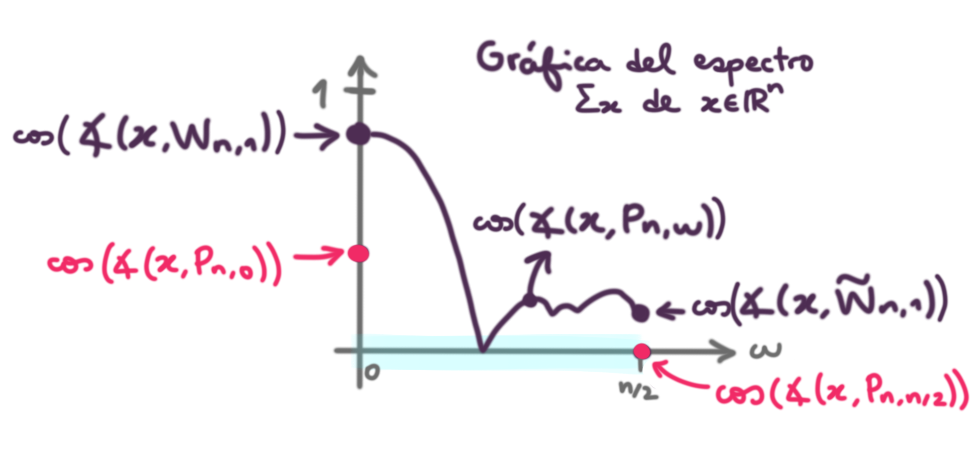
\includegraphics[scale = 1.5]{esp_ang} 
\end{figure}	

\begin{comment}
Esta última proposición es importante, pues relaciona
el espectro de una señal 
con sus primeros dos coeficientes respecto a la base
de Legendre discreta $\cali{L}^{n}$. \\
Note que este es un resultado razonable, pues, por
definición del espectro $\Sigma_{x}$, si $\omega \geq 0$,
$\Sigma_{x}(\omega)$ es el coseno del ángulo que
$x$ forma con el espacio $P_{n, \omega} = 
span \left\{ cos \left(
2 \pi \omega\frac{m}{n}
\right)_{m=0}^{n-1},  
sen \left(
2 \pi \omega\frac{m}{n}
\right)_{m=0}^{n-1} \right\}$, y, conforme
$\omega$ tiende a cero por la derecha, 
las discretizaciones de coseno y seno que generan
el espacio $P_{n, \omega}$ tienden a ser las discretizaciones
de cosenos y senos de muy baja frecuencia, luego, intuitivamente
son las discretizaciones de las rectas tangentes de un coseno
y un seno en $t =0$, que son las rectas $y=1$
y $y =x$. Observe que discretizaciones de estas dos rectas
conforman una base para el espacio $W_{n,1}$.
\end{comment}
\section{Simetría, periodicidad y continuidad del espectro $\Sigma_{x}$}
\label{sec: simetria, periodicidad, continuidad}
Fijada una dimensión $n \geq 2$,
si $x \in \IR^{n}$ es cualquier señal y 
$\Sigma_{x}$
es su espectro como se definió en
\ref{def: espectro monofrecuenciales},
en esta sección vamos a demostrar 
algunos resultados sobre la periodicidad 
de esta función y su simetría 
respecto a puntos de la forma
$\frac{n}{2} \IZ$.
Esto será de utilidad pues nos permitirá
acotar considerablemente el dominio de frecuencias
de $\Sigma_{x}$.



\begin{prop}
\label{prop: periodicidad espectro}
\textbf{(Periodicidad del espectro)}
Sean $n \geq 2$, $x \in \IR^{n}$.
Sea $\Sigma_{x}$ el espectro de $x$ como se definió en 
\eqref{def: espectro monofrecuenciales inicial}.
El espectro $\Sigma_{x}$ es $n-$periódico, es decir, 
para cualquier frecuencia
$0 \leq \omega \leq n$
y toda $K \in \IZ$, se tiene que 
\[
\sigma_{n}(x, \omega) = \sigma_{n}(x, \omega + Kn).
\]
\end{prop}
\noindent
\textbf{Demostración.}
Sólo observe que 
\begin{align*}
\tilde{c}_{n, \omega + Kn} = & \left( cos \left( 2 \pi
\left( \omega + Kn \right) \frac{m}{n} \right) \right)_{m=0}^{n-1} \\
= & \left( cos \left( 
2 \pi \omega \frac{m}{n} + 2 \pi K m
\right) \right)_{m=0}^{n-1} \\
= & \left( cos \left( 
2 \pi \omega \frac{m}{n}
\right) \right)_{m=0}^{n-1} = \tilde{c}_{n, \omega}
\end{align*}
y, similarmente, que 
\[
\tilde{s}_{n, \omega + Kn} = \tilde{s}_{n, \omega},
\]
luego, por definición de los espacios monofrecuenciales
(c.f. ecuación \ref{eq: espacio Pnw}),
\begin{align*}
P_{n, \omega + Kn} =
& span(\tilde{c}_{n, \omega + Kn}, \tilde{s}_{n, \omega + Kn}) \\
= & span(\tilde{c}_{n, \omega }, \tilde{s}_{n, \omega }) = P_{n, \omega};
\end{align*}
de esto se concluye, usando la definición
\ref{def: final de sigmas},
que 
\[
\sigma_{n}(x, \omega) = 
cos (\measuredangle(x, P_{n, \omega}))
= cos (\measuredangle(x, P_{n, \omega + Kn})) = 
\sigma_{n}(x, \omega + Kn).
\]
\QEDB
\vspace{0.2cm}

\begin{figure}[H]
	\sidecaption{
	Según la periodicidad establecida en la proposición 
	\ref{prop: periodicidad espectro}, basta calcular los
	coeficientes espectrales
	$\sigma_{n}(x, \omega)$ para frecuencias
	$0 \leq \omega \leq n$.
	\label{fig: periodicidad espectro}
	}
	\centering
	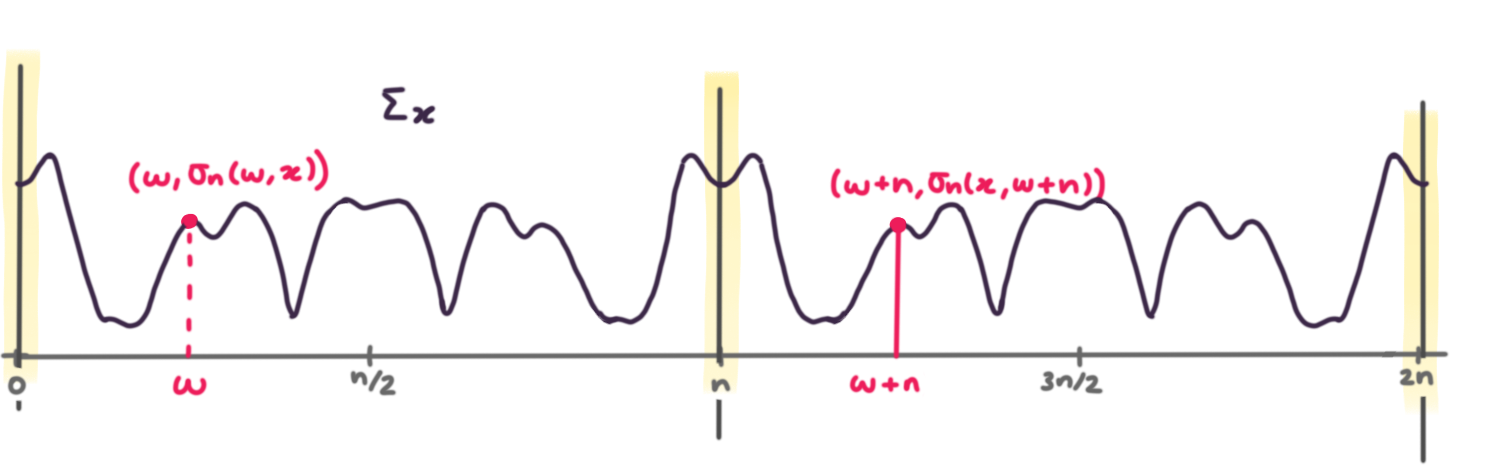
\includegraphics[scale = 0.9]{periodicidad_espectro} 
\end{figure}	


\begin{prop}
\textbf{(Simetría del espectro)}
Sean
$n \geq 2$,
$x \in \IR^{n}$. Para toda $0 \leq1 \omega \leq \frac{n}{2}$,
\[
\sigma_{n}(x, \omega) = 
\sigma_{n}(x, n-\omega ). 
\]
\end{prop}
\noindent
\textbf{Demostración.}
En efecto, 
\begin{align*}
\tilde{c}_{n, \omega + n} = & \left( cos \left( 2 \pi
\left( n- \omega \right) \frac{m}{n} \right) \right)_{m=0}^{n-1} \\
= & \left( cos \left( 
2 \pi n \frac{m}{n} - 2 \pi \omega
\frac{m}{n}
\right) \right)_{m=0}^{n-1} \\
= & \left( cos \left( 
2 \pi m - 2 \pi \omega \frac{m}{n} 
\right) \right)_{m=0}^{n-1} \\
= & \left( cos \left( 2 \pi \omega \frac{m}{n} \right) \right)_{m=0}^{n-1}
= \tilde{c}_{n, \omega}
\end{align*}
y, similarmente,
\[
\tilde{s}_{n, \omega + Kn} = -\tilde{s}_{n, \omega};
\]
de esto, como en la demostración de la proposición
\ref{prop: periodicidad espectro}, se concluye la igualdad
entre los espacios $P_{n, \omega}$ y $P_{n, n-\omega}$, y de esto
la igualdad deseada.
\QEDB
\vspace{0.2cm}

\begin{figure}[H]
	\sidecaption{
	Podemos así afinar la afirmación hecha en la figura 
	\ref{fig: periodicidad espectro} y concluir que basta
	calcular los coeficientes
	$\sigma_{n}(x, \omega)$ para $0 \leq \omega \leq \frac{n}{2}$,
	pues los demás pueden deducirse a partir de reflexiones y traslaciones.
	\label{fig: simetria espectro}
	}
	\centering
	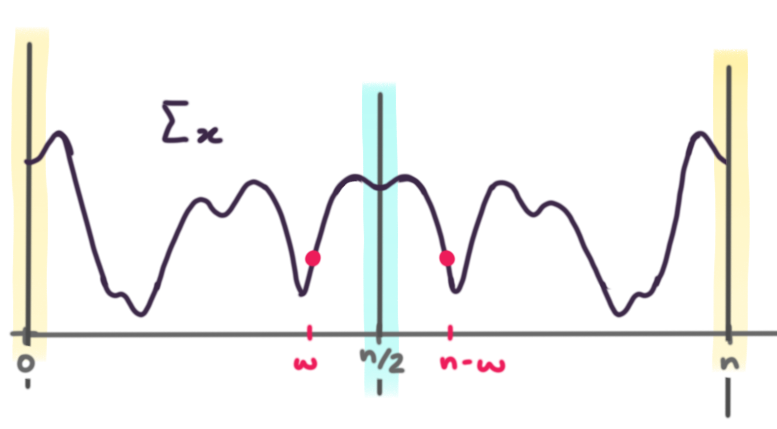
\includegraphics[scale = 1.4]{simetria_espectro} 
\end{figure}	
 

\begin{nota}
\label{nota: muestreo dom frecuencia}
Según estas propiedades de periodicidad y simetría,
podemos limitarnos a evaluar el espectro
$\Sigma_{x}$ de una señal sólo en frecuencias
contenidas en el intervalo $[0, n/2]$, pues los valores
del espectro para otros valores pueden deducirse por periodicidad
y simetría. \\

Ahora bien, para poder escribir programas
para calcular un tal espectro $\Sigma_{x}$
se debe de usar
un conjunto discreto de puntos.
Para los espectros que calcularemos de ahora en 
adelante, adoptamos la convención de 
usar usar como dominio 
del espectro
$\Sigma_{x}$ de una señal $x \in \IR^{n}$
al conjunto
\TODO{revisa!}
\begin{equation}
\label{eq: malla frecuencias}
\left\{ \frac{a}{100} : \hspace{0.2cm}
0 \leq a \leq \frac{100n}{2} \right\},
\end{equation}

es decir, se toman $100$ muestras por
cada unidad del intervalo 
$\left[ 0, \frac{n}{2}\right]$
\end{nota}


Para terminar, hagamos algunos comentarios
sobre la continuidad del espectro $\Sigma_{x}$
de una señal $x \in \IR^{n}$. \\
Por definición del espectro, 
si $\omega \geq 0$, entonces
$\Sigma_{x}(\omega) = \sigma_{n} (x, \omega)$,
donde los coeficientes
$\sigma_{n} (x, \omega)$ son como se definieron en
la proposición \ref{prp: ammm}.
Por la periodicidad y simetría del espectro, basta
analizar la continuidad de $\Sigma_{x}$ sólo en el
intervalo cerrado $[0, n/2]$. \\

Observe que la fórmula
\eqref{eq: coef sigma caso 1}, que sirve
para calcular $\sigma_{n} (x, \omega)$
cuando $\omega \in ]0, n/2[$, es una combinación
de sumas y productos de senos y cosenos
evaluados en funciones de la frecuencia $\omega$, luego, 
es una función continua, por lo tanto $\Sigma_{x}$
es continua en el interior del intervalo 
$[0, n/2]$. No pudimos determinar la
continuidad de $\Sigma_{x}$ en los puntos
extremos $0$ y $n/2$, ni encontramos un criterio que deba
cumplir la señal que implique la continuidad en uno
de estos puntos extremos.
No escribimos en detalle los intentos para
determinar los límites
\[
\limite{\omega \rightarrow 0^{+}}{\sigma_{n}(x, \omega)}
\hspace{0.2cm} \textit{y} \hspace{0.2cm}
\limite{\omega \rightarrow \frac{n}{2}^{-}}{\sigma_{n}(x, \omega)},
\]
pero comentamos que el problema que encontramos fue
intentar determinar el límite
(cuando $\omega \rightarrow 0^{+}$ y cuando $\omega \rightarrow \frac{n}{2}^{-}$)
de la expresión
\[
\sqrt{2} \left(
n - \frac{sen(2 \pi \omega) cos (2 \pi \omega \frac{n-1}{n})}{sen(2 \pi \omega/n)}
\right)^{-1/2}
\cdot
\suma{m=0}{n-1}{x_{m} sen(2 \pi \omega m/n)};
\]
puesto que se tiene una indeterminación de tipo
$\infty \cdot 0$, se aplicó la Regla de L'Hôpital
(c.f. \cite{hopital}) 
para intentar determinar el límite, pero esto sólo
nos llevó a una expresión más complicada que presentaba una indeterminación
de tipo $\frac{0}{0}$. No esperabamos que la tarea
de determinar la continuidad por los extremos fuese sencilla,
pues después de graficar algunos espectros notamos que algunos
de ellos eran continuos por ambos extremos, mientras que otros
presentaban discountinuidades (que, por estár acotados los valores
del espectro por $0$ y $1$, necesariamente son de salto)
en uno o ambos extremos, y no notamos características de 
la señal $x$ a partir de la cual se calcula el espectro
que indicaran cuándo se tenía la discontinuidad por uno 
de los puntos extremos.





\section{Relación entre los espectros basados en la TDF y en espacios monofrecuenciales}

Después de todo lo expuesto en las secciones anteriores, tenemos
ya dos alternativas para realizar un análisis
espectral de una señal $x \in \IR^{n}$.

Sean $n \geq 2$, $M := \lceil \frac{n}{2} \rceil$, $x \in \IR^{n}$.
\begin{itemize}
	\item \textbf{(Espectro-0: basado en la TDF)} 
	Usando la transformada discreta de Fourier
	(c.f. sección \ref{sec: TDF}),
	el espectro de $x$ es la función
	\[
	\Tau_{x}: Dom_{TDF, n} \longrightarrow \IR^{+}_{0}
	\]	
	definida en \ref{def: espectro DFT}.
	
	La gráfica es entonces la de las frecuencias
	enteras $\omega$ dadas (dependiendo de la 
	paridad de $n$) por las
	tablas 6.1 y 6.2
	versus los coeficientes
	$\tau_{n}(x, \omega)$ definidos en
	\ref{def: taus}.
	
	Puesto que el realizar un análisis de 
	$x$ via la TDF significa encontrar una
	expresión de $x$ como una suma
	ponderada de muestreos de senos y cosenos,
	de frecuencias enteras las indicadas en las tablas 6.1 o 6.2,
	se tiene que  
	\begin{itemize}
		\item Para toda frecuencia $\omega$ considerada
		por la TDF,
		\[
		0 \leq \tau_{n}(x, \omega) \leq 1,
		\]
		y que
		\item entre más se acerque
		$\tau_{n, \omega}(x)$
		a $1$, mayor es la
		importancia de la frecuencia $\omega$ para
		sintetizar s $x$; recíprocamente, si 
		$\tau_{n}(x, \omega)$ es cercana a cero, entonces
		la frecuencia $\omega$ no es muy relevante para 
		sintetizar a la señal $x$.
	\end{itemize}
	\begin{defi}
	\label{def: FM0}
	Llamaremos \textbf{frecuencia principal-0}
	(y denotaremos por $FP0(x)$) 
	a una 
	frecuencia $\omega \in Dom_{TDF, n}$
	tal que, para cualquier otra $\omega' \in Dom_{TDF, n}$ 
	se tenga que 
	\[
	\tau_{n}(x, \omega') = \Tau_{x}(\omega^{'}) \leq
	\Tau_{x}(\omega) =  
	 \tau_{n}(x, \omega).
	\]
	\end{defi}
	Observe que tal frecuencia principal existe por ser 
	el máximo de un conjunto finito de números, pero que no 
	estamos asegurando que sea única. 
	
	\item \textbf{(Espectro-1: basado en espacios monofrecuenciales)} 
	Usando
	las ideas propuestas en 
	la sección
	\ref{sec: metodologia para realizar un analisis espectral que considere frecuencias arbitrarias}, 
	es decir, si se usan cosenos de ángulos a
	espacios monofrecuenciales $P_{n, \omega}$
	(c.f. \ref{eq: espacio Pnw}), el espectro
	de una señal $x$ se definió en
	\ref{def: espectro monofrecuenciales inicial}
	como la función 
	\[
	\Sigma_{x} : \left[0, \frac{n}{2} \right] \longrightarrow [0,1].
	\]
	
	La gráfica de este espectro es la de 
	las frecuencias $\omega \in [0, \frac{n}{2}]$ versus	
	los coeficientes
	$\sigma_{n}(x, \omega)$ definidos en 
	\ref{prp: ammm}. Observe que
	\begin{itemize}
		\item para cualquier frecuencia $\omega \geq 0$, se tiene que
		\[
		0 \leq \sigma_{n}(x, \omega) \leq 1
		\]
		\item 
	y, el que
	$\sigma_{n}(x, \omega)$ sea cercano a $1$ significa que un
	muestreo uniforme de un sinusoide de frecuencia $\omega$
	modela bien el comportamiento de $x$,
	mientras que un $\sigma_{n}(x, \omega)$ cercano
	a cero significa que 
	$x$ es casi perpendicular a toda señal de frecuencia $\omega$
	(c.f. nota \ref{nota: significado de los sigma en AE}).
	\end{itemize}
\end{itemize}

Nos gustaría, así como hicimos en la definición
\ref{def: FM0}, definir la frecuencia principal 
de una señal $x$ basada en el espectro
$\Sigma_{x}$ de esta. No es tan sencillo hacer esto, pues,
como comentamos en la sección
\ref{sec: simetria, periodicidad, continuidad}, no parece
que para toda señal $x \in \IR^{n}$ el espectro
$\Sigma_{x}$ sea continuo en los puntos extremos
$0$ y $n/2$, por lo que intentar definir una
frecuencia principal como
\[
\omega \in [0, n/2] \textit{ tal que }
a_{x} = \Sigma_{x}(\omega), \textit{ donde }
a_{x} = sup \{ \Sigma_{x}(w): \hspace{0.2cm} \omega
\in [0, n/2] \}
\]
no es adecuado, pues no está excluida la 
posibilidad de que exista un espectro $\Sigma_{x}$
para el que no exista una $\omega \in [0, n/2]$ 
tal que $\Sigma_{x}(\omega) = a_{x}$, o sea, tal que 
$a_{x}$ que no sea máximo
del conjunto 
$\{ \Sigma_{x}(w): \hspace{0.2cm} \omega
\in [0, n/2] \}$. \\

\begin{figure}[H]
	\sidecaption{
	Se muestra un dibujo hipotético de un espectro
	$\Sigma_{x}$ para el que $a_{x} = 1$ pero no exista
	ninguna frecuencia $\omega \geq 0$ (una candidata
	a frecuencia principal) tal que $\Sigma_{x}(\omega) = a_{x}$.
 	\label{fig: ej FP1}
	}
	\centering
	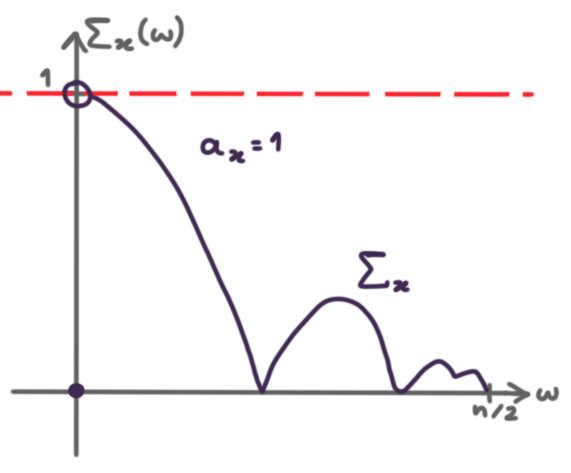
\includegraphics[scale = 1]{ejemplo_FP1.png} 
\end{figure}	
Sorteamos este problema si restringimos las frecuencias
$\omega$ a considerar a un subconjunto finito del
rango inicial de frecuencias
$[0, n/2]$.

\begin{defi}
	\label{def: FM1}
	Sean $n \geq 2$, $x \in \IR^{n}$. Sea
	$\cali{P}$ un subconjunto finito
	de $[0, n/2]$.
	Llamaremos la \textbf{frecuencia principal-$1$}
	(y denotaremos
	por $FP1(x)$) 
	de $x$ respecto al conjunto $\cali{P}$	
	a una frecuencia $\omega \in \cali{P}$ 
	tal que, para cualquier otra $\omega'$ del $\cali{P}$, se tenga que
	\[
	\sigma_{n, \omega'}(x) = \Sigma_{x}(\omega') 
	\leq \Sigma_{x}(\omega) = \sigma_{n, \omega}(x).
	\]
\end{defi}
En la práctica, el que se tenga que fijar un conjunto
finito $\cali{P} \subseteq [0, n/2]$ de frecuencias
para calcular la FP1 no es un problema, pues ya teníamos que hacer
esto para calcular, de forma computacional, el espectro
$\Sigma_{x}$. Para respetar la convención
puesta en la nota 
\ref{nota: muestreo dom frecuencia}, vamos
a tomar a $\cali{P}$ como en 
\eqref{eq: malla frecuencias}.
	
\begin{nota}
Observe que no estamos asegurando
que las frecuencias principales
$FP0(x)$ y $FP1(x)$ como se definieron en 
\ref{def: FM0} y \ref{def: FM1}
sean únicas.
Si hay dos o más frecuencias $\omega'$ que satisfagan
la definición de frecuencia principal-0 
(resp. frecuencia principal-1), tomamos
como valor de $FP0(x)$ 
(resp. $FP1(x)$)
a la mayor de tales $\omega'$.
\end{nota}


Demostremos ahora que, de hecho, el espectro-0
de hecho es la restricción del espectro-1
al conjunto de frecuencias 
$Dom_{TDF, n}$ considerado por la transformada discreta
de Fourier.
\begin{prop}
\label{prop: coinciden espectr}
Sean $n \geq 2$, $x \in \IR^{n}$.
Sea $Dom_{TDF, n}$ el dominio del espectro-0 de $x$
como se definió en \ref{def. Dom tdf}. Se tiene que
\begin{equation}
\label{eq4: 4May}
\forall \omega \in Dom_{TDF, n}:
\hspace{0.2cm} \tau_{n}(x, \omega) = \sigma_{n}(x, \omega).
\end{equation}
\end{prop}

\noindent
\textbf{Demostración.}
Recuerde que los coeficientes
$\sigma_{n}(x, \omega)$
se definieron como
\[
\sigma_{n}(x, \omega) = \frac{|| \Pi_{P_{n, \omega}}(x) ||}{|| x ||}.
\]
Teniendo una base ortonormal del espacio 
$P_{n, \omega}$ puede calcularse la proyección involucrada en la fórmula
para $\sigma_{n}(x, \omega)$.
Recuerde que, por definición del espacio $P_{n, \omega}$,
\begin{itemize}
	\item los vectores $c_{n, \omega}$ y $s_{n, \omega}$ conforman
	una base de $P_{n, \omega}$ cuando $1 \leq \omega \leq M-1$ 
	(pues, para estos valores de omega se tiene siempre
	que $\omega \not\in \frac{n}{2} \IZ$) y
	\item $c_{n, \omega}$ conforma una base 
	de $P_{n, \omega}$ cuando $\omega = 0$ y,
	en el caso en el que $n$ es par, también para cuando $\omega = M$
	(pues sólo para estos valores de omega se tiene 
	que $\omega \in \frac{n}{2} \IZ$).
\end{itemize}
Además, según la proposición
\ref{prop: base de fourier version real},
para todas estas $\omega$,
los vectores de la lista anterior son ortogonales entre
sí y tienen norma uno, luego, más que una base de 
$P_{n, \omega}$ constituyen una BON para este espacio.
Así, $\Pi_{P_{n, \omega}}(x)$ puede encontrarse 
simplemente calculando los productos punto 
de $x$ con los elementos de estas BONs (c.f. 
nota \ref{nota: sobre la identidad de parseval});
comparando este cálculo con la definición 
\ref{def: taus}
de los coeficientes $\tau_{n}(x, \omega)$,
concluimos que en efecto se
tiene la iguadad \eqref{eq4: 4May}.

\QEDB
\vspace{0.2cm}

Así, \textbf{el espectro basado en espacios monofrecuenciales
es una extensión de la definición del espectro 
basado en la transformada discreta de Fourier}.
Como ya recordamos al inicio, la
ventaja de este primer espectro es que para calcularlo es posible usar
un rango cualquiera de frecuencias no negativas, mientras que el segundo, 
a pesar de que da no sólo un proceso de análisis de una señal 
de $x$ a partir de sinusoides, sino también uno de síntesis
(c.f. nota \ref{nota: ya?}), se limita a considerar las frecuencias 
en $Dom_{TDF, n}$. \\

Recuerde que en la nota 
\ref{nota: muestreo dom frecuencia} explicamos que 
basta evaluar a $\Sigma_{x}$ en el intervalo $[0, n/2]$, 
pues a partir de estos valores puede deducirse el valor
del espectro en cualquier otra frecuencia positiva; observe que,
para toda $n$, el conjunto de frecuencias enteras 
consideradas por la TDF, $Dom_{TDF, n}$, está
contenido en $[0, n/2]$, luego, basta calcular 
a $\Sigma_{x}$ en $[0, n/2]$
para tener ambos análisis espectrales.


\begin{nota}
\label{nota: la mejor frecuencia}
Fijados $n \geq 2$
y $x \in \IR^{n}$, \textbf{entre más cercano a $1$ sea 
el coeficiente 
$\sigma_{n}(x, \omega)$, mejor es usar un sinusoide
de frecuencia $\omega$ para ajustar la gráfica de $x$}.
Esto porque, recuerde, entre más cercano a uno sea uno de
esos coeficientes, más cercana estará la señal $x$ 
al espacio monofrecuencial $P_{n, \omega}$, luego, más
cercana está $x$
a tener
la propiedad de ser una discretización de un sinusoide
de la respectiva frecuencia $\omega$.
\end{nota}

\begin{nota}
\label{nota: proyeciones monof TDF}
Sea $x \in \IR^{n}$; sea 
\eqref{ec: sintesis 0} o 
\eqref{ec: sintesis 1}
(dependiendo de la paridad de $n$)
la síntesis de $x$ respecto a la base de Fourier
real $\cali{F}_{n}$. De esta suma, podemos
separar los sumandos que corresponden a una
cierta frecuencia $\omega \in Dom_{TDF, n}$; recordando
que, como se notó
en la demostración de la proposición
\ref{prop: coinciden espectr}, 
los correspondientes vectores
de frecuencia $\omega$ (que son ya sea uno o dos, dependiendo del valor
de $\omega$) conforman una BON para el correspondiente
espacio monofrecuencial 
$P_{n, \omega}$, tenemos que la parte de la 
síntesis de $x$ que corresponde a 
cierta frecuencia $\omega$ es igual a
$\Pi_{P_{n, \omega}}(x)$. \\

Aplicando esto al ejemplo \ref{ej: DFT1},
si $x$ es la señal definida en 
\ref{eq2: 10ab}, se tiene que
\[
\Pi_{7, 0} = 4.12 c_{7,0}, 
\]
\[
\Pi_{7, 1} = -8.76 c_{7,1} - 7.35 s_{7,1}, 
\]
\[
\Pi_{7, 2} = 4.77 c_{7,2} - 10 s_{7,2}, 
\]
\[
\Pi_{7, 3} = 0.14 c_{7,3} + 9.91 s_{7,z3}.
\]
\end{nota}



\begin{ejemplo}
\label{ej: espectros comparacion}

Sea $f_{\omega}$
el sinusoide definido como
\begin{equation}
\label{eq: sinusoide eje}
f_{\omega}(t) := -1.5 cos (2 \pi \cdot \omega t + 2 \pi \cdot 0.2).
\end{equation}
Considere a una señal $x \in \IR^{16}$ que sea el resultado
de muestrear uniformemente al sinusoide
$f_{3.4}$
con ruido aleatorio 
(con distribución, pongamos, uniforme en $[-0.5, 0.5]$).

A continuación, mostramos las gráficas
de los espectros de $x$. Para
calcular el espectro $\Sigma_{x}$,
usamos el dominio
establecido en la nota 
\ref{nota: muestreo dom frecuencia}.

\begin{figure}[H]
\centering
	\sidecaption{ De ahora en adelante, siempre que
	grafiquemos espectros,usaremos los colores y notaciones
	de esta figura. \label{fig: ejemplo_comparacion}}
    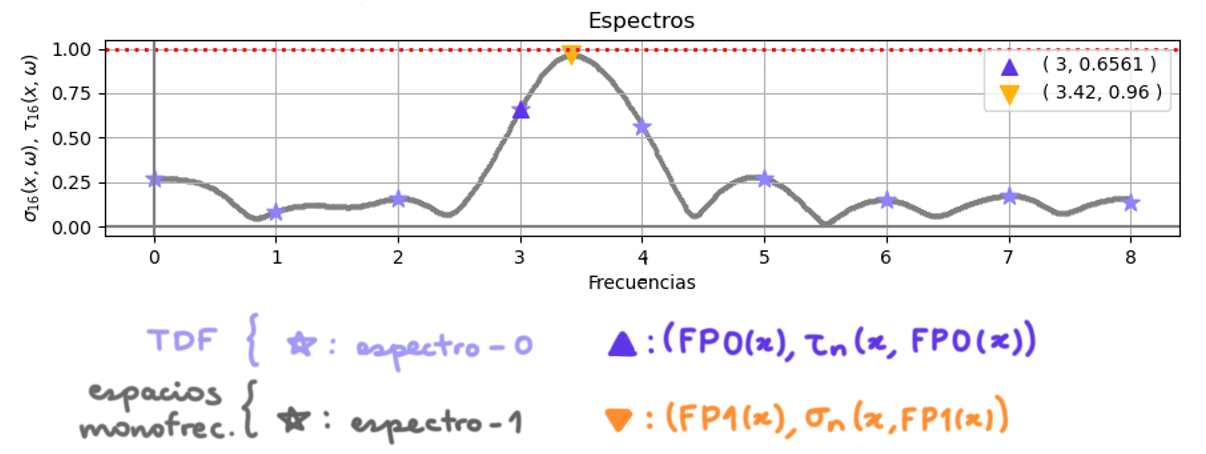
\includegraphics[scale = 1]{./estudios_espectrales/ejemplo_comparacion_1}
\end{figure}


Observe cómo el espectro-$1$ parece completar la información
dada por el espectro-$0$, pues, a diferencia del primero,
el espectro-$0$
da coeficientes de frecuencia $\tau_{n}(x, \omega)$ sólo
para algunas frecuencias enteras $\omega$, mientras que en el espectro-$1$
es posible considerar cualesquiera frecuencias $\omega \geq 0$; como puede observar
en la gráfica, 
\[
FP0 (x) = 3 \hspace{0.2cm} \textit{y} \hspace{0.2cm}
FP1 (x) = 3.42;
\]
esta segunda frecuencia es mucho más cercana a
la frecuencia $\omega =3.4$ del sinusoide del que
fue obtenida la señal $x$; como agregamos ruido
aleatorio en las mediciones, no 
es de extrañarse que no se haya
obtenido exactamente $FP1(x) = 3.4$.

A pesar de que el espectro-$0$, el obtenido a partir de la
transformada discreta de Fourier, no dio una mala estimación (del rango
de frecuencias $Dom_{TDF,n}$ considerado por esta herramienta,
$\omega =3$ es el valor más cercano al valor real $\omega = 3.4$), vemos en este
ejemplo que usando el espectro-$1$ es posible obtener mejores
estimaciones de frecuencias que modelen a la señal original. \\

Mostramos ahora la gráfica de $x$ junto con
\begin{itemize}
	\item la parte de la síntesis de $x$ respecto a la $TDF$
	que corresponde a la frecuencia principal
	$FP0(x)$ (c.f.
	nota \ref{nota: ya?}), que de hecho,
	según la nota \ref{nota: proyeciones monof TDF}, es
	$\Pi_{P_{36,3}}(x)$
	\begin{figure}[H]
			\sidecaption{
			Puesto que $\{ c_{36, 3}, s_{36, \omega} \}$
			es una BON de $P_{36, 3}$, claro que la señal 
			que resulta de discretizar el sinusoide morado en la malla
			$I_{36}$ es, de hecho, la proyección de $x$ 
			al espacio monofrecuencial $P_{36, 3}$.
 			\label{fig: comparacion 2}
			}
			\centering
			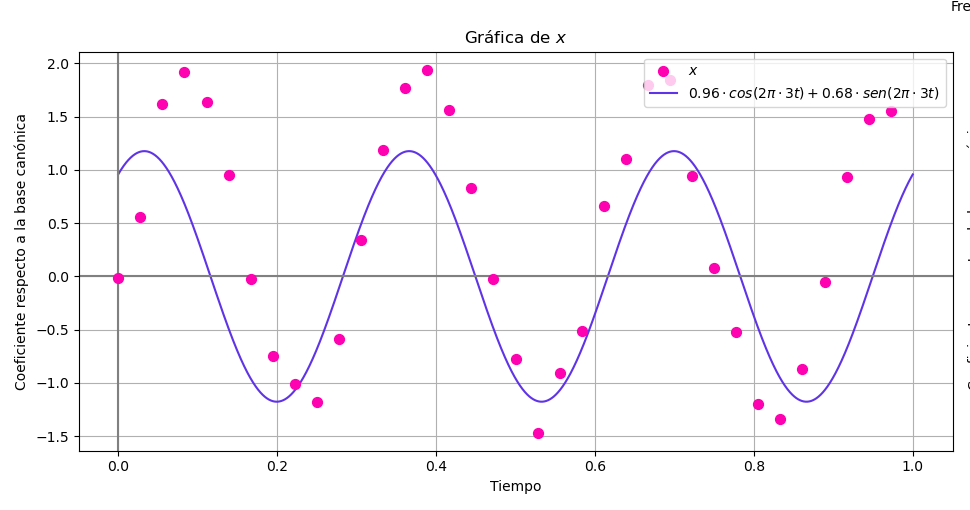
\includegraphics[scale = 0.5]{./estudios_espectrales/ejemplo_comparacion_2} 
		\end{figure}		
	
	y
	\item la señal $\Pi_{P_{16, 3.42}}(x)$, o sea, la señal de
	dimensión $16$ y frecuencia $FP1(x)=3.42$ más cercana a $x$, junto con
	el sinusoide continuo del que fue muestreado.
	\begin{figure}[H]
			\sidecaption{
			Para obtener la versión continua del sinusoide 
			discreto $\Pi_{P_{36, 3.42}}(x)$ (i.e. la gráfica naranja),
			usamos las fórmulas establecidas en los teoremas
			\ref{teo: amelie1} y \ref{teo: amelie2}.
			\label{fig: comparacion 3}
			}
			\centering
			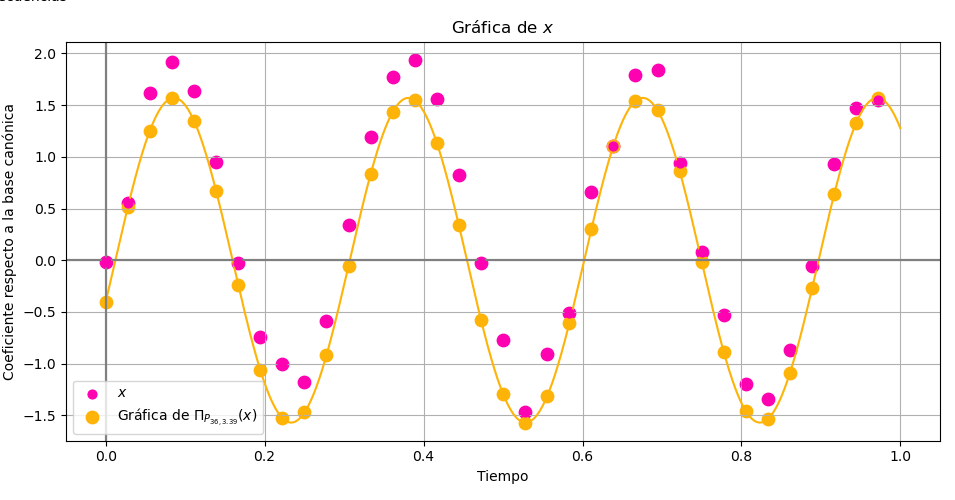
\includegraphics[scale = 0.5]{./estudios_espectrales/ejemplo_comparacion_3} 
		\end{figure}		
\end{itemize}


Los sinusoides de las figuras \ref{fig: comparacion 2} y
\ref{fig: comparacion 3}
son las señales de frecuencia pura
$3$ y $3.42$, respectivamente, cuya distancia euclidea
a la señal original $x$ es mínima. Observe que la segunda
señal, aquella cuya frecuencia
fue determinada
a partir del estudio espectral basado en espacios
monofrecuenciales,
parece ajustarse un poco mejor a la gráfica de $x$. \\

\begin{figure}[H]
			\sidecaption{
			Mostramos ahora los espectros de la señal $x$ que se obtiene
			tomando $36$ muestras uniformemente espaciadas del mismo sinusoide
			$f_{3.4}(t)$, 	
			esta vez sin agregar ruido aleatorio a las mediciones.
			Observe que el espectro-1 detectó a la frecuencia $\omega = 3.4$
			como la mejor, y que el sinusoide naranja ajusta perfectamente la gráfica
			de $x$. Como la frecuencia real no es entera, usar la frecuencia principal
			dada por la TDF sigue sin dar resultados perfectos, aunque no malos.
			\label{fig: sinusoide sin ruido}
			}
			\centering
			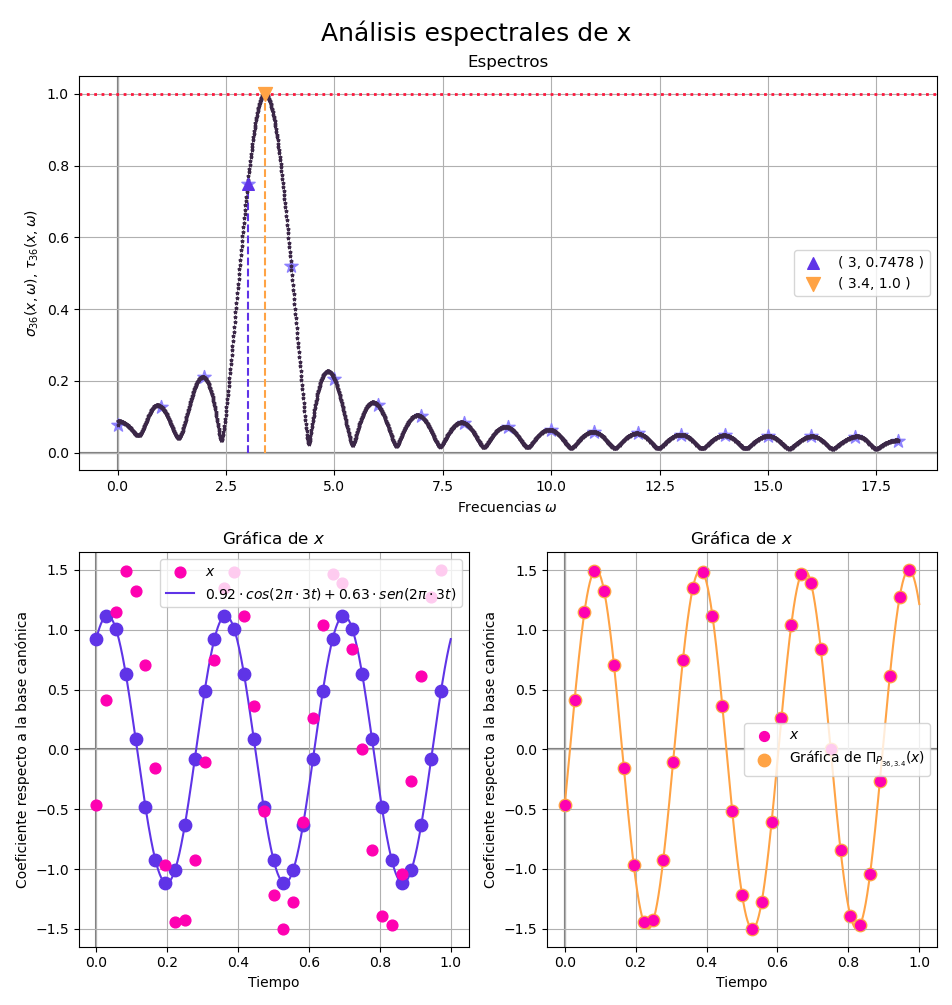
\includegraphics[scale = 0.4]{./estudios_espectrales/sinusoide_sin_ruido} 
		\end{figure}		



	\begin{figure}[H]
			\sidecaption{
			Si ahora muestreamos sin ruido
			del sinusoide $f_{5}$,
			como 
			era de esperarse, la frecuencia principal de ambos
			espectros es $5$
			(y el valor de los 
			espectros en tal frecuencia
			es igual a $1$, la cota
			superior). Además, 
			las gráficas de frecuencia $5$ que resultan
			ajustan a la perfección a la señal original $x$.
			\label{fig: comparacion 4}
			}
			\centering
			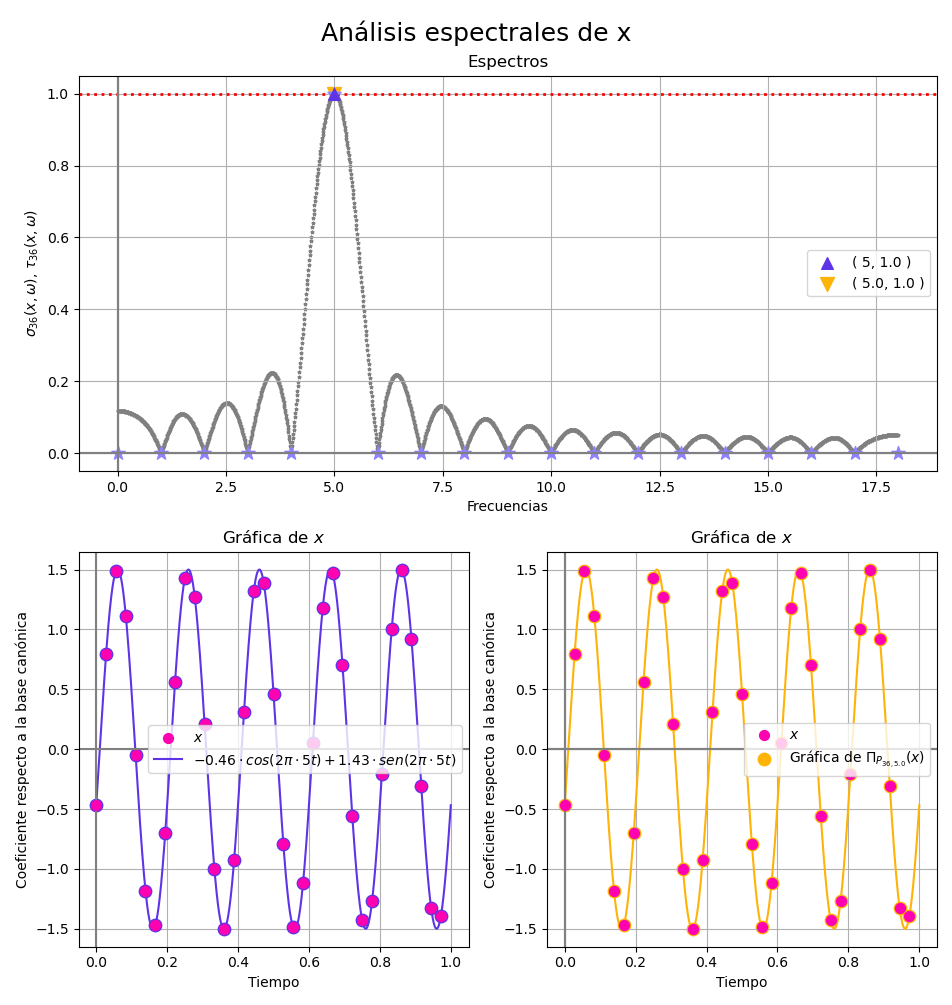
\includegraphics[scale = 0.4]{./estudios_espectrales/ejemplo_comparacion_4} 
		\end{figure}	


Para terminar este ejemplo, tomemos una suma de sinusoides
de varias frecuencias, digamos, de frecuencias
$1$, $4$ y $7$; sea
\[
g(t) = 3 sen(2 \pi t) + sen(2 \pi \cdot 4t) + 0.5 cos(2 \pi \cdot 7t).
\]
Sea $x$ la señal que resulta de muestrar, sin ruido, este sinusoide
$g$, siendo $25$ el tamaño de la muestra.
\begin{figure}[H]
	\sidecaption{
	En la imagen se muestran los espectros de tal $x$. Observe que los
	espectros parecen concentrarse alrededor de las 
	frecuencias $1$, $4$ y $7$.
	\label{fig: sin varias frec}
	}
	\centering
	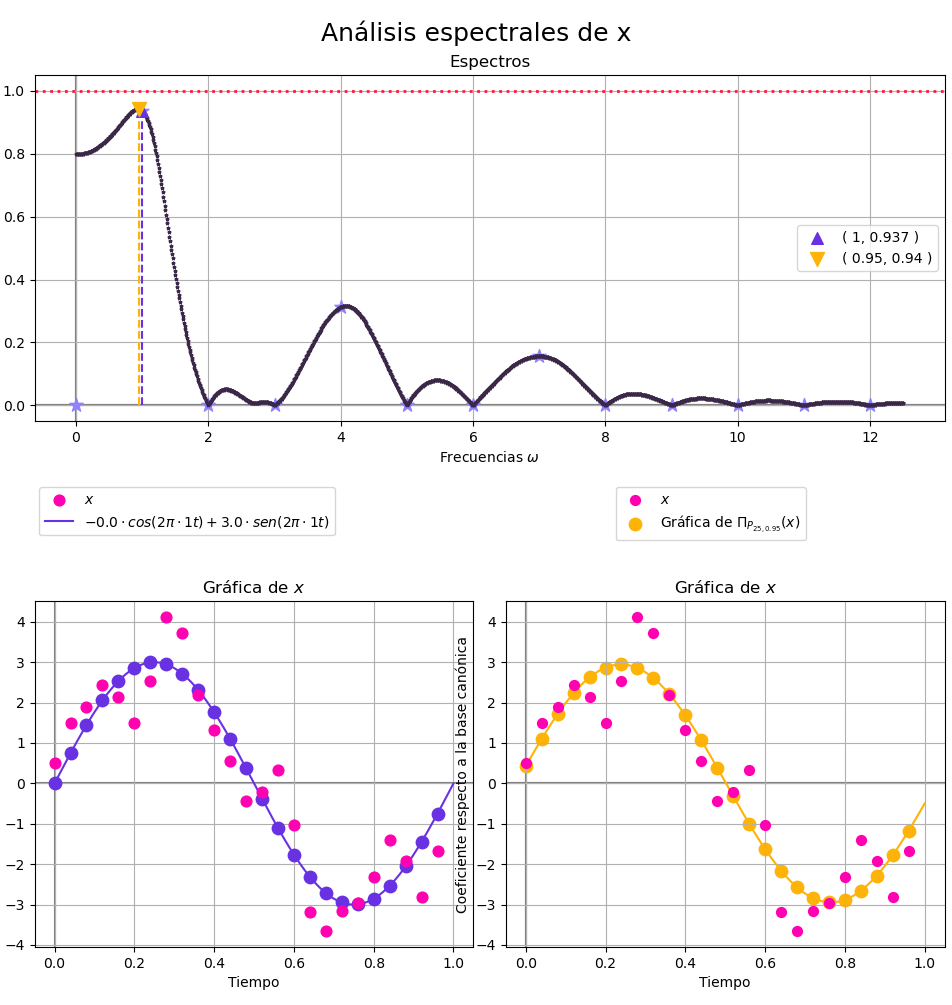
\includegraphics[scale = 0.4]{./estudios_espectrales/sinusoide_varias_frecuencias} 
\end{figure}	

\final
\end{ejemplo}

\subsection{Adaptación del análisis espectral a señales reales con una frecuencia de muestreo dada}

Para hacer nuestros análisis espectrales, hemos
usado la dimensión $n$ del PDL $\cali{L}^{n, k} \in \IR^{n}$
en cuestión
para buscar, en base a máximos globales
del espectro 
$\Sigma_{x}: [0, \frac{n}{2}] \longrightarrow [0,1]$, la
mejor frecuencia $\omega$ para aproximar la gráfica
de $\cali{L}^{n,k}$ en base a un sinusoide discreto
de dimensión $n$. \\


Note que en esa discusión nunca hablamos de 
parámetros importantes para, de forma canónica, hacer
un análisis espectral, como lo son la
duración en tiempo de la señal o la frecuencia
de muestreo.

\begin{defi}
\label{def: tiempo y frec de muestreo}
La cantidad de muestras tomadas (de forma uniforme)
de una señal por unidad de tiempo 
será denotada por $F_{s}$ y llamada \textbf{frecuencia
de muestreo} de la señal. A la cantidad de unidades de
tiempo que dura la medición se le denotará por $T$. \\

A la cantidad total de muestras tomadas se le denotará
por $L$.
\end{defi}
Observe que, para poder dividir una unidad
de tiempo en $F_{s}$ subintervalos de igual longitud,
se deben divider al eje del tiempo con los puntos
\begin{equation}
t_{k} := t_{0} + h k, \hspace{0.2cm}
\textit{con } h := \frac{1}{F_{s}}.
\end{equation}
A tal constante $h$, definida como el recíproco de la frecuencia
de muestreo, se le llama el \textbf{paso temporal} de la señal. \\

De las definiciones se sigue de inmediato que
\begin{equation}
\label{eq: relacion L, T Fs}
L = T F_{s}.
\end{equation}
\begin{figure}[H]
	\sidecaption{
	Adoptamos la convención de empezar a medir 
	un bloque de $F_{s}$ mediciones desde que inicia la
	unidad de tiempo (que, en el caso de la figura, se ha
	fijado como segundos).
	\label{fig: Fs 1}
	}
	\centering
	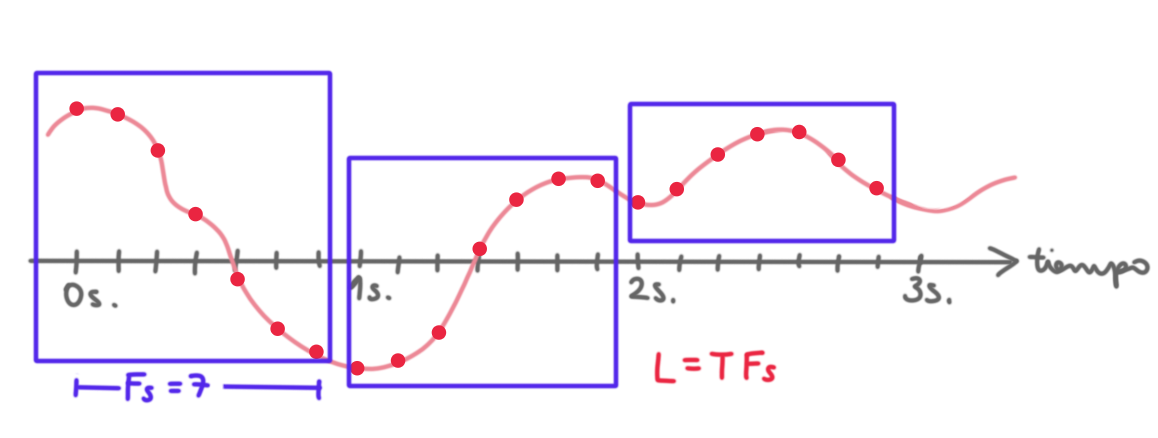
\includegraphics[scale = 1]{Fs_1} 
\end{figure}	

Nosotros, por el momento, sólo nos
hemos enfocado en buscar
una frecuencia $\omega \in [0, \frac{n}{2}]$ que de lugar
a un sinusoide que aproxime bien la gráfica
de $\cali{L}^{n,k}$;
observe que, al hacer esto, hemos supuesto de forma
implícita que estamos estudiando una señal
de duración una unidad de tiempo
($T = 1$) de longitud $n$
(o sea, $L = F_{s} = n$). \\
Supongamos ahora que
tenemos una señal $x$ que consta de $L$ mediciones, siendo
$F_{s}$ la frecuencia de muestreo.
\begin{figure}[H]
	\sidecaption{
	Para la imagen, hemos fijado $F_{s}= 10$
	y $L = 40$.
	\label{fig: frecuencia 1}
	}
	\centering
	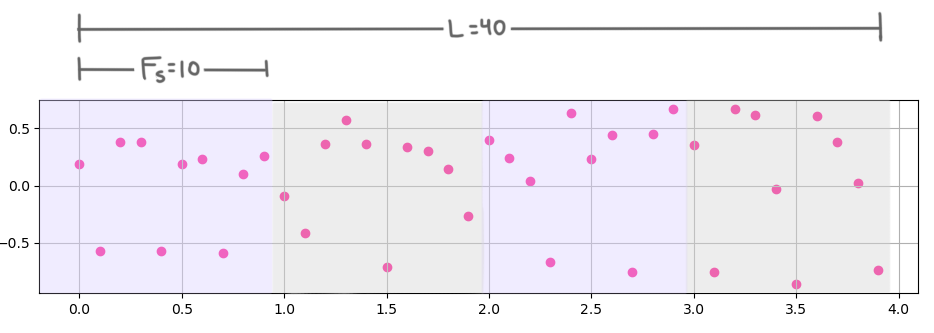
\includegraphics[scale = 0.45]{frecuencia_1} 
\end{figure}	

Sea ahora $2 \leq n \leq L$ y
supogamos que
se hizo el análisis
espectral 
de una sección $x_{|n}$ de tal señal
que conste de $n$ puntos
(usando el espectro
$\Sigma_{x}: [0, \frac{n}{2}]
\longrightarrow [0,1]$).
Digamos que, como conclusión de ese análisis, se
obtuvo que un sinusoide de frecuencia $\omega \in [0, \frac{n}{2}]$
ajusta bien \textit{esa sección particular 
$x_{|n}$
de la señal $x$}.
\begin{figure}[H]
	\sidecaption{
	Para la imagen, hemos fijado $n= 6$;
	se calculó que la mejor frecuencia para ajustar 
	los primeros $6$ puntos que componen la señal
	original $x$ es $w = 2$.
	\label{fig: frecuencia 2}
	}
	\centering
	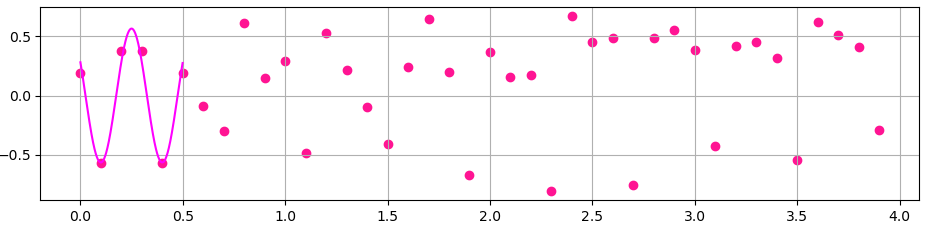
\includegraphics[scale = 0.45]{frecuencia_2} 
\end{figure}	

Observe que, en general, si se quisiera usar
directamente una frecuencia de $w$ para ajustar
a la señal $x$, la aproximación lograda en los
$n$ puntos escogidos previamente puede no ser válida.
\begin{figure}[H]
	\sidecaption{
	Usando los datos de la figura \ref{fig: frecuencia 2}, podriamos
	intentar en un principio usar a un sinusoide de frecuencia $2$
	para intentar modelar a la señal, pero un sinusoide de tal frecuencia,
	como es el caso de esta figura, puede que ni siquiera sea adecuado
	para modelar el pedazo $x_{|n}$ original a partir del cual se obtuvo
	la frecuencia $\omega$.
	\label{fig: frecuencia 2}
	}
	\centering
	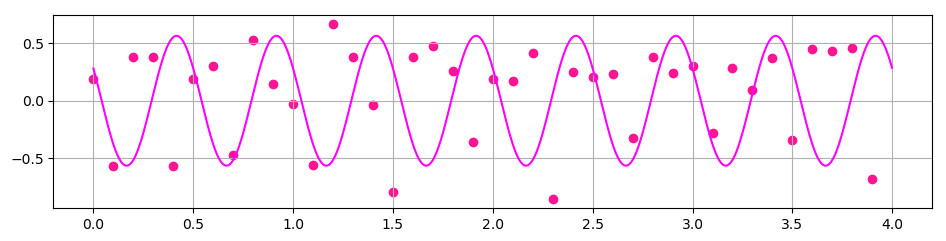
\includegraphics[scale = 0.45]{frecuencia_3} 
\end{figure}
Esto se debe a que	
tal frecuencia $\omega$ es buena para aproximar
a dichos $n$ puntos cuando se ha tomado como
unidad de tiempo a $n$, pero, 
por la forma en que fue muestreada la señal original $x$,
son $F_{s}$ (y no necesariamente $n$) la cantidad de puntos
que conforman una unidad. Así, puesto que con $\omega$
ciclos de un sinusoide se aproximaron $n$ puntos, 
la frecuencia que debe escogerse para aproximar a todos los $L$
puntos es
\begin{equation}
\label{eq: rel frecuencia real y ficticia}
\tilde{w} := \frac{F_{s}}{n} \omega.
\end{equation}

\begin{figure}[H]
	\sidecaption{
	Es con una simple regla de tres que se deduce
	la relación \eqref{eq: rel frecuencia real y ficticia}.
	\label{fig: frecuencia real}
	}
	\centering
	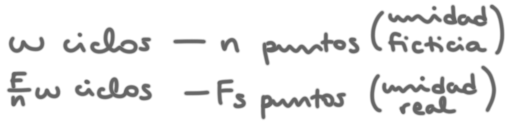
\includegraphics[scale = 1.4]{frecuencia_real} 
\end{figure}	
\begin{figure}[H]
	\sidecaption{
	Según los datos de las figuras
	\ref{fig: frecuencia 1}
	y \ref{fig: frecuencia 2}, con un sinusoide de frecuencia
	$\tilde{\omega} = 10/3$ se aproximan bien a los seis
	puntos en base a los cuales se encontró a la primera
	frecuencia $\omega$.
	\label{fig: frecuencia 4}
	}
	\centering
	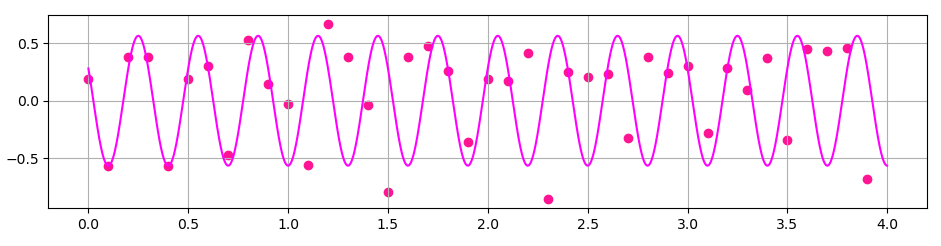
\includegraphics[scale = 0.45]{frecuencia_4} 
\end{figure}
\section{PROVISIONAL; límites}

En \TODO{rojo} se resaltan las fórmulas que YA se han
verificado calculándolas dos veces. En 
\textcolor{blue}{azul} cuando la aproximación ha sido
simulada exitosamente.


\TODO{
\[
\frac{sen(2 \pi \omega) cos(2 \pi \omega \frac{n-1}{n})}{sen
(2 \pi \frac{\omega}{n})}
\sim
\frac{
2 \pi \omega - \frac{4 \pi^{3}}{3n^{2}}
(4n^2-6n+3) \omega^{3} + o(\omega^{5})
}{
\frac{2\pi}{n} \omega -
\frac{4 \pi^{3}}{3 n^{3}} \omega^{3} + o(\omega^{5})
},
\]
}
por lo que

\textcolor{blue}{
\begin{align*}
\xi_{n, \omega} \sim &
\sqrt{2} 
\left(
4 \pi
\frac{                                                                                                                                          
\omega - \frac{2\pi^{2}}{3n^{2}}(2n^2-3n+2)\omega^{3} + o(\omega^{5})
}{
\frac{2\pi}{n} \omega -
\frac{4 \pi^{3}}{3 n^{3}} \omega^{3} + o(\omega^{5})
}
\right)^{-1/2} \\
\sim &
\sqrt{2} 
\left(
2n
\frac{                                                                                                                                          
\omega - \frac{2\pi^{2}}{3n^{2}}(2n^2-3n+2)\omega^{3} + o(\omega^{5})
}{
\omega -
\frac{2 \pi^{2}}{3 n^{2}} \omega^{3} + o(\omega^{5})
}
\right)^{-1/2} 
\rightarrow \frac{1}{\sqrt{n}},
\end{align*}
}

\textcolor{blue}{
\begin{align*}
\eta_{n, \omega} \sim &
\sqrt{2} 
\left(
\frac{
8 \pi^{3} (2n-1)(n-1)\omega^{3} + o(\omega^{5})
}{
6 \pi n \omega -
\frac{4 \pi^{3}}{n} \omega^{3} + o(\omega^{5})
}
\right)^{-1/2} \\
\sim & 
\sqrt{2} 
\left(
4\pi^{2}
\frac{
(2n-1)(n-1)\omega^{3} + o(\omega^{5})
}{
3 n \omega -
\frac{2 \pi^{2}}{n} \omega^{3} + o(\omega^{5})
}
\right)^{-1/2} 
 \rightarrow \infty.
\end{align*}
}

\textcolor{blue}{
\begin{align*}
\langle
c_{n, \omega}, s_{n, \omega}
\rangle \sim &
\frac{2\pi}{n}
\xi_{n, \omega} \eta_{n, \omega}
(n-1)  
\left(
\frac{n}{2} \omega - \frac{2\pi^{2}}{3} (n-1) \omega^{3} + o(\omega^{5})
\right) \\
= & 
\frac{2 \sqrt{2}}{n \sqrt{n}} \pi (n-1)
\left(
\frac{
\frac{3}{2} \pi n^{3}\omega^{3} + o(\omega^{5})
}{
8 \pi^{3}(2n-1)(n-1)\omega^{3} + o(\omega^{5})
}
\right)^{1/2}
\rightarrow \frac{
\sqrt{6(n-1)}
}{2 \sqrt{2n-1}}.
\end{align*} 
}
Tuve que usar la expresión asintótica
de $\eta_{n, \omega}$ para poder determinar este
último límite, pues con la expresión de la
primera linea tenía una indeterminación
de tipo $\infty \cdot 0$.

\textcolor{blue}{
\[
\langle x,
c_{n, \omega}
\rangle = 
\xi_{n, \omega} 
\left(
X_{0} - \frac{2 \pi^{2}}{n^{2}}X_{2} \omega^{2} 
+ \frac{2 \pi^{4}}{3n^{4}} X_{4} \omega^{4} + o(\omega^{5})
\right) \rightarrow \frac{X_{0}}{\sqrt{n}} ,
\]
}

\textcolor{blue}{
\begin{align*}
\langle x,
s_{n, \omega}
\rangle = &
\eta_{n, \omega} 
\left(
\frac{2 \pi}{n} X_{1} \omega - \frac{4 \pi^{3}}{3n^{3}}X_{3} \omega^{3} 
 + o(\omega^{5})
\right)\\
= &
\begin{cases}
\sqrt{2} \left(
\frac{
\frac{24 \pi^{3}}{n}X_{1}^{2}\omega^{3} + o(\omega^{5}) }{
8 \pi^{3} (2n-1)(n-1)\omega^{3} + o(\omega^{5})
}
\right)^{1/2}
\rightarrow \left(
\frac{6 X_{1}^{2}}{(2n-1)(n-1)n}
\right)^{1/2} & \textit{si } \alpha_{n, \omega}(x) \geq 0 \\
-\sqrt{2} \left(
\frac{
\frac{24 \pi^{3}}{n}X_{1}^{2}\omega^{3} + o(\omega^{5}) }{
8 \pi^{3} (2n-1)(n-1)\omega^{3} + o(\omega^{5})
}
\right)^{1/2}
\rightarrow -\left(
\frac{6 X_{1}^{2}}{(2n-1)(n-1)n}
\right)^{1/2} & \textit{si } \alpha_{n, \omega}(x) < 0,\\
\end{cases}
\end{align*}
}
donde
\[
\alpha_{n, \omega}(x) := 
\frac{2 \pi}{n} X_{1} \omega - \frac{4 \pi^{3}}{3n^{3}}X_{3} \omega^{3}.
\] 

\TODO{Ya lo tengo. Lo único no tan lindo de la fórmula
es que se requiere calcular el signo del coeficiente alpha. No sé si 
sea siempre fácil de determinar-o si quiera
si sea constante cerca de cero. Lo que yo hice en el programa es determiar
el signo para cuando $\omega = 0.001$}





\begin{equation}
\label{ec: limite x, cnw}
\limite{\omega \rightarrow 0^{+}}{\langle
x, c_{n, \omega}
\rangle }
= \frac{X_{0}}{\sqrt{n}}
\end{equation}

\begin{equation}
\label{ec: limite x, snw}
\limite{\omega \rightarrow 0^{+}}{\langle
x, s_{n, \omega}
\rangle }
\begin{cases}
\left(
\frac{6 X_{1}^{2}}{(2n-1)(n-1)n}
\right)^{1/2} & \textit{si } \alpha_{n, \omega}(x) \geq 0 \\
-\left(
\frac{6 X_{1}^{2}}{(2n-1)(n-1)n}
\right)^{1/2} & \textit{si } \alpha_{n, \omega}(x) < 0,\\
\end{cases}
\end{equation}

\begin{equation}
\label{ec: limite -2abc}
\limite{\omega \rightarrow 0^{+}}{
-2 \langle x, c_{n, \omega} \rangle
\langle x, s_{n, \omega} \rangle
\langle c_{n, \omega}, s_{n, \omega} \rangle
= 
}
\end{equation}

Así, los elementos que parecen en la fórmula
para $\sigma_{n}(x, \omega)$ cuando $\omega \not\in \frac{n}{2} \IZ$ son
\begin{itemize}
\item 
\TODO{
\[
\langle
c_{n, \omega}, s_{n, \omega}
\rangle^{2} \sim
\frac{4\pi^{2}}{n^{2}}(n-1)^{2} \xi_{n, \omega}^{2} \eta_{n, \omega}^{2}
\left(
\frac{n^{2}}{4} \omega^{2} - \frac{2n}{3} \pi^{2} (n-1) \omega^{4} + o(\omega^{5})
\right)
\]
}
sigue desarrollando el eta  !!!
\item
\TODO{
\[
\langle x,
c_{n, \omega}
\rangle^{2} = 
\xi_{n, \omega}^{2}
\left(
X_{0}^{2} - \frac{4 \pi^{2}}{n^{2}}X_{0}X_{2} \omega^{2} 
+ 
\frac{4 \pi^{4}}{n^{4}}
\left(
\frac{1}{3} X_{0}X_{4} + X_{2}^{2}
\right) \omega^{4} 
+ o(\omega^{5})
\right)
\]
}

\item
\TODO{
\[
\langle x,
s_{n, \omega}
\rangle^{2} = 
\frac{4 \pi^{2}}{n^{2}}
\eta_{n, \omega}^{2}
\left(
X_{1}^{2}\omega^{2} - \frac{4 \pi^{2}}{3n^{2}}X_{1}X_{3} \omega^{4} 
+  o(\omega^{5})
\right)
\]
}

\item
\[
\langle
x, c_{n, \omega}
\rangle
\langle
x, s_{n, \omega}
\rangle
\langle
c_{n, \omega}, s_{n, \omega}
\rangle \sim
\frac{2 \pi^{2}}{n}
\xi_{n, \omega}^{2} \eta_{n, \omega}^{2}(n-1)
\left(
X_{0}X_{1}\omega^{2} 
- \frac{2 \pi^{2}}{n}
\left(
\frac{1}{3n} X_{0}X_{3} + \frac{1}{n} X_{2}X_{1}
+ \frac{2}{3}(n-1)X_{0}X_{1}
\right) \omega^{4}
\right).
\]
\end{itemize}

\TODO{Cambia los iguales por $\sim$.}
Según estos cálculos, si
$a_{n, \omega} = \langle x, c_{n, \omega} \rangle$, 
$b_{n, \omega} = \langle x, s_{n, \omega} \rangle$, 
$c_{n, \omega} = \langle c_{n, \omega}, s_{n, \omega} \rangle$, 
entonces

\[
a_{n, \omega}^{2} + b_{n, \omega}^{2} - 
2a_{n, \omega}b_{n, \omega}c_{n, \omega}
= N_{1} + N_{2} +N_{3},
\]
donde

\[
N_{1} =
\xi_{n, \omega}^{2} \left(
X_{0}^{2} - \frac{4\pi^{2}}{n^{2}} X_{0}X_{2}
\omega^{2} + \frac{4 \pi^{4}}{n^{4}}
\left(
\frac{1}{3} X_{0}X_{4} + X_{2}^{2}
\right) \omega^{4}
\right)
\rightarrow 
\frac{X_{0}}{n}
\left(
X_{0}  - \frac{4 \pi^{2}}{n^{2}}X_{2}
\right),
\]

\[
N_{2} = \frac{4 \pi^{2}}{n^{2}} \eta_{n, \omega}^{2}
\left(
X_{1}^{2} \omega^{2} - \frac{4 \pi^{2}}{3n^{2}}X_{1}X_{3} \omega^{4}
+ o(\omega^{5})
\right)
=
\frac{16 \pi^{3}}{n^{2}}
\frac{3n \omega - \frac{2 \pi^{2}}{n} \omega^{3} + o(\omega^{5})}{
8 \pi^{3}(2n-1)(n-1) \omega^{3} + o(\omega^{5})
}
\rightarrow \infty,
\]

\[
N_{3} =
\frac{-4 \pi^{2}}{n}
\xi_{n, \omega}^{2} \eta_{n, \omega}^{2}(n-1)
\left(
X_{0}X_{1}\omega^{2} 
- \frac{2 \pi^{2}}{n}
\left(
\frac{1}{3n} X_{0}X_{3} + \frac{1}{n} X_{2}X_{1}
+ \frac{2}{3}(n-1)X_{0}X_{1}
\right) \omega^{4}
\right)
\rightarrow ?,
\]
luego, no puedo determinar este último límite, por lo tanto,
tampoco hablar solbre el límite de
de $a_{n, \omega}^{2} + b_{n, \omega}^{2} - 
2a_{n, \omega}b_{n, \omega}c_{n, \omega}$, pues
tengo una indeterminación del tipo 
$0 \cdot \infty$. \\

El denominador es
\[
1-c^{2} \sim
1 - \frac{4\pi^{2}}{n^{2}}(n-1)^{2} \xi_{n, \omega}^{2} \eta_{n, \omega}^{2}
\left(
\frac{n^{2}}{4} \omega^{2} - \frac{2n}{3} \pi^{2} (n-1) \omega^{4} + o(\omega^{5})
\right) \rightarrow ?,
\]
aquí también tengo una indeterminación de tipo
$0 \cdot \infty$.


\chapter{Análisis espectrales: resultados numéricos}
\label{chap: resultados numericos analisis espectrales}

Después de todo lo expuesto en las secciones anteriores, tenemos
ya dos alternativas para graficar el espectro
de una señal $x \in \IR^{n}$.

\begin{itemize}
	\item Usando la transformada discreta de Fourier
	(c.f. sección \ref{sec: TDF}), el espectro de
	una señal $x$ es la gráfica de las frecuencias
	enteras dadas (dependiendo de la 
	paridad de $n$) por las
	tablas 6.1 y 6.2
	versus los coeficientes
	$\tau_{n}(x)$ definidos en
	\ref{def: taus}.
	\TODO{Puesto que hacer un análisis con la
	DFT significa expresar a $x$ como una suma
	ponderada de muestreos de senos y cosenos
	de algunas frecuenicas enteras,...}
	
	\item Si, para hacer un análisis espectral, se usan
	las ideas propuestas en 
	la sección
	\ref{sec: metodologia para realizar un analisis espectral que considere frecuencias arbitrarias}, entonces, dado un rango de frecuencias 
	$\omega$,
	el espectro de $x$ es la gráfica de 
	las frecuencias $\omega$ versus	
	los coeficientes
	$\sigma_{n}(x, \omega)$.
	

\TODO{a diferencia de la dft, los casos extremos ya no son
estar o no estar, sino ser perpendicular o ser paralelo a su
representante del espacio monofrecuencial.}
\end{itemize}

Espectro cero: el de TDF
Espectro uno: el de espacios monofrecuenciales

\begin{figure}[H]
	\sidecaption{
	Ejemplo de los espectros resultantes
	de los dos métodos de análisis.
	\label{fig: espectro 1 }
	}
	\centering
	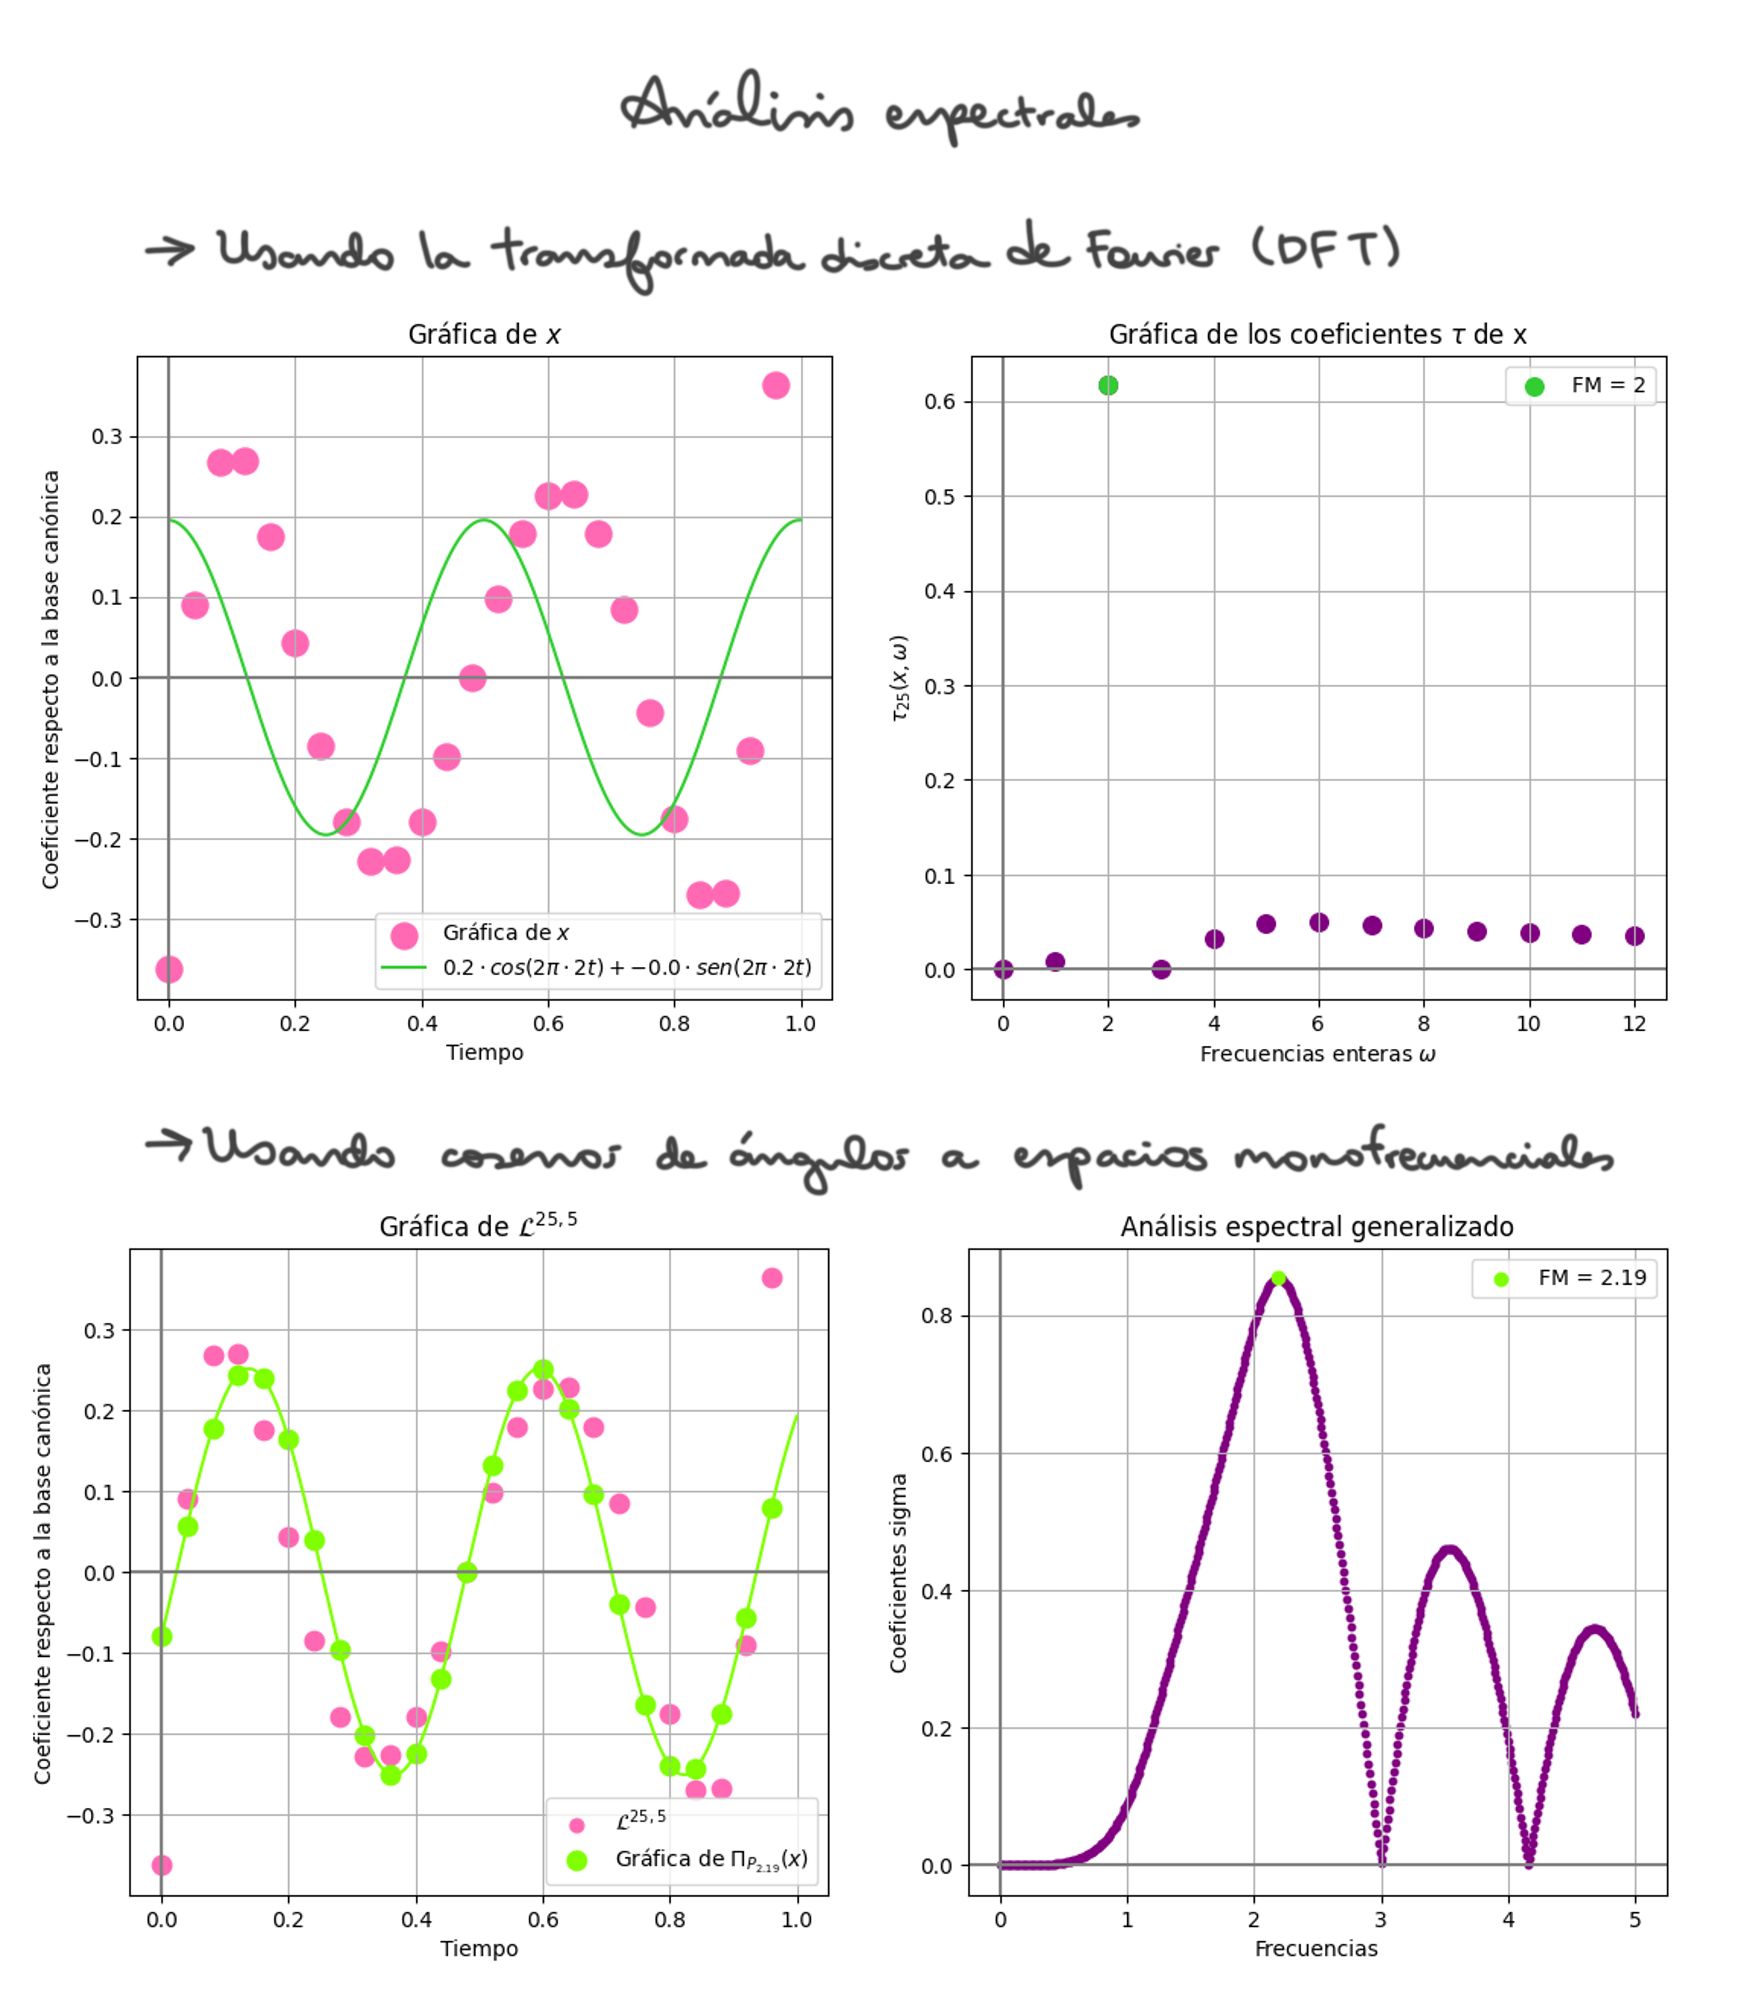
\includegraphics[scale = 1]{ejemplo_analisisEspectrales} 
\end{figure}	

\section{Lista de preguntas a responder usando los resultados numéricos}

\begin{notacion}
Dados los espectros cero y uno de $\cali{L}^{n,k}$, si
$FM_{i}$ 
(para $i=0,1$)
es la frecuencia $\omega$ en la que el espectro 
$i$ alcanza su punto máximo.
\TODO{cambia esto en los cpódgios}
\end{notacion}


Enlistamos las preguntas que nos interesa considerar
(formuladas de manera general, pero que comprobaremos o refutaremos
numéricamente para dimensiones hasta $n=70$, pues para dimensiones
más grandes los errores computacionales son demasiado grandes
como para obtener conclusiones fiables, \TODO{revisa lo que tiene que
decir al respecto el libro de data science!}).

Vamos a responder estas preguntas con gráficas!

La primera pregunta es una reformulación de la 
hipótesis \ref{ref: hipotesis}. Hacemos dos preguntas
más para afinar.

\begin{itemize}
\item \textbf{Pregunta 1}: 
Para cualesquiera $n \geq 2$ y $0 \leq k \leq n-1$,
¿ocurre que las frecuencias máximas
$FM_{0}$ y $FM_{1}$ son cercanas a $\frac{k}{2}$?

\begin{figure}[H]
	\sidecaption{
	\TODO{Voy a responder esta con algunas imágenes de espectros como esta.}
	\label{fig: ejemplo_pregunta1}
	}
	\centering
	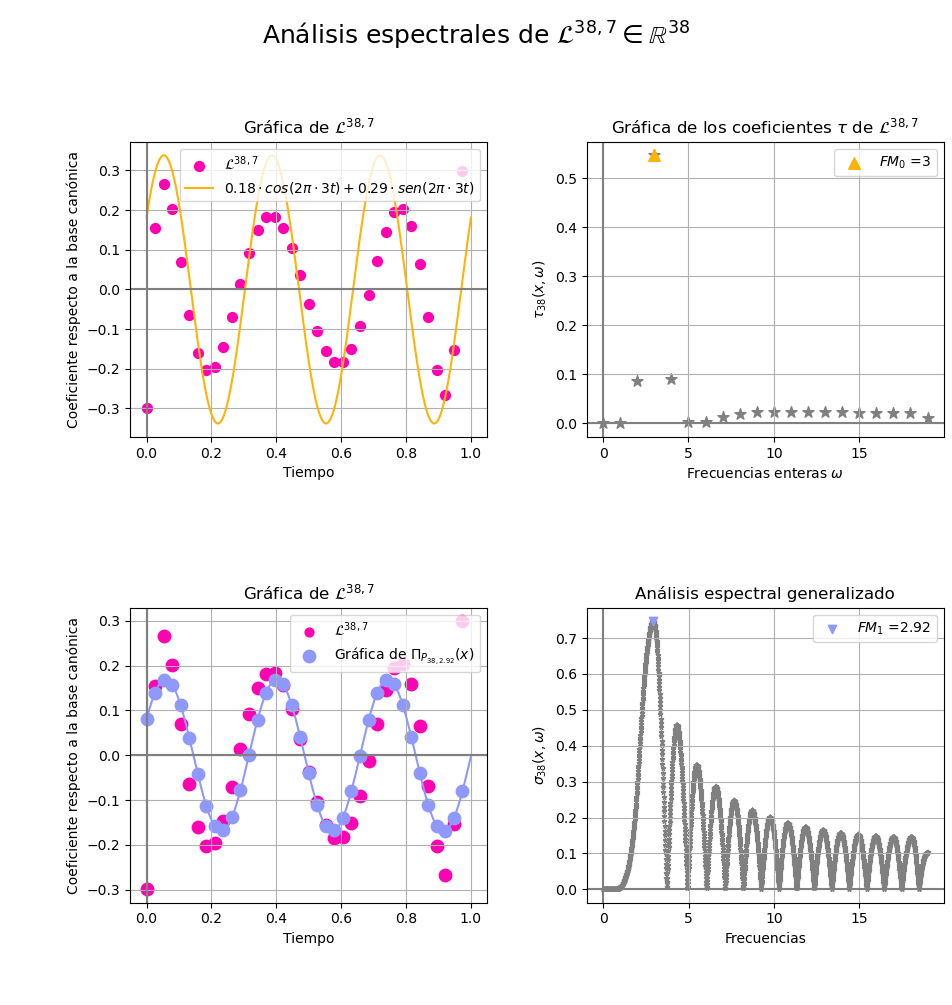
\includegraphics[scale = 0.5]{./estudios_espectrales/ejemplo_pregunta1} 
\end{figure}	

\item \textbf{Pregunta 2}: ¿En efecto dependen $FM_{0}$ y $FM_{1}$ sólo
de $k$ y no de $n$?

\begin{figure}[H]
	\sidecaption{
	\TODO{Voy a responder esta con algunas imágenes de espectros como esta.}
	\label{fig: ejemplo_pregunta2}
	}
	\centering
	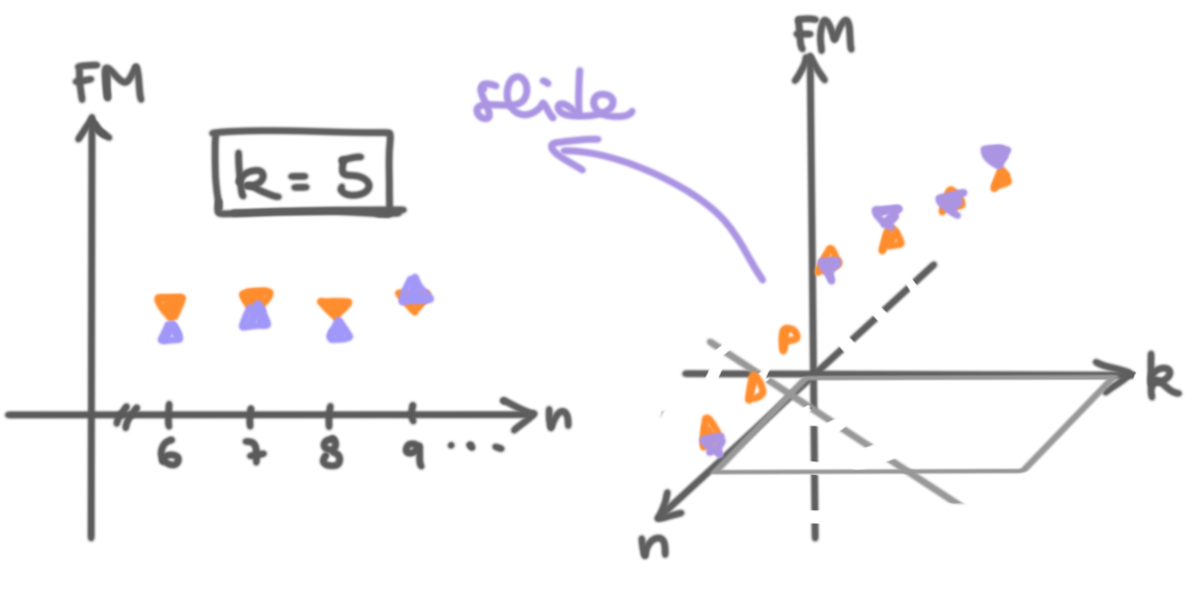
\includegraphics[scale = 1]{./estudios_espectrales/ejemplo_pregunta2} 
\end{figure}	

\item \textbf{Pregunta 3}: ¿Los parámetros $(m,b)$ de pendiente y ordenada al 
origen de las rectas de mínimos cuadrados (RMC) de las gráficas 
de FM para un $n$ fijo son parecidos? ¿En dónde se concentran?
\TODO{reformula mejor. Esta pregunta es para mejor la estimación dada
en la hipótesis!}
\begin{figure}[H]
	\sidecaption{
	\TODO{Voy a responder esta con algunas imágenes de espectros como esta.}
	\label{fig: ejemplo_pregunta3}
	}
	\centering
	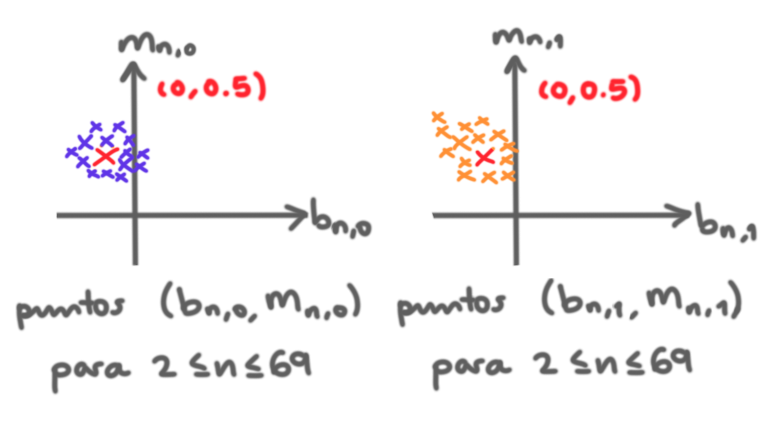
\includegraphics[scale = 1]{./estudios_espectrales/ejemplo_pregunta3} 
\end{figure}	
\end{itemize}

Note que las preguntas 2 y 3 son más bien globales
(y las respondo numéricamente con los datos calculados en 
la función \texttt{analisis$\_$espectralPDL$\_$global}).